% LaTeX Template for short student reports.
% Citations should be in bibtex format and go in references.bib
\documentclass[a4paper, 11pt]{article}
\usepackage[top=3cm, bottom=3cm, left = 2cm, right = 2cm]{geometry}
\geometry{a4paper}
\usepackage{fontspec}
\usepackage{xeCJK}
\setmonofont{Victor Mono}[Scale=0.9]
\makeatletter
\renewcommand*\verbatim@nolig@list{}
\makeatother
\usepackage[utf8]{inputenc}
\usepackage{textcomp}
\usepackage{graphicx}
\usepackage{quiver}
\usepackage{ottalt}
\usepackage{amsmath,amssymb,bbm,amsthm,extarrows}
\usepackage{algorithm}
\usepackage{algpseudocode}
\usepackage{bm}
\usepackage{subcaption,float}
\usepackage{mathpartir}
\usepackage{stmaryrd}
\usepackage{xspace}
\usepackage{minted}
\usepackage[bookmarks,colorlinks,breaklinks]{hyperref}
%\hypersetup{linkcolor=black,citecolor=black,filecolor=black,urlcolor=black} % black links, for printed output
\usepackage{memhfixc}
\usepackage{fancyhdr,fancyvrb}
\usepackage{booktabs}
\pagestyle{fancy}
\theoremstyle{remark}\newtheorem*{remark}{Remark}
\theoremstyle{definition}\newtheorem*{definition}{Definition}
\newtheorem{theorem}{Theorem}
\title{Mid-Term Report}
\author{高振明/Zhenming Gao}
%\date{}

\input{doublebrackets}
\newcommand{\sem}[1]{\llbracket #1 \rrbracket}
\newcommand{\semK}[2]{\llbracket #1 \rrbracket_{#2}}
\newcommand{\Lam}{\mathsf{L}}
\newcommand{\CPS}{\mathsf{C}}
\newcommand{\Val}{\mathsf{Val}}
\newcommand{\Ans}{\mathsf{Ans}}
\newcommand{\Env}{\rho}
\newcommand{\Kont}{\kappa}
\newcommand{\FunTab}{\Phi}
\newcommand{\KontTab}{\Phi_\kappa}
\newcommand{\halt}{\mathsf{halt}}
\newcommand{\app}{\mathsf{app}}
\newcommand{\appK}{\mathsf{appK}}
\newcommand{\ite}{\mathsf{ite}}
\newcommand{\letone}{\mathbf{let}_1}
\newcommand{\letK}{\mathbf{letK}}
\newcommand{\letRec}{\mathbf{let\;rec}}
\newcommand{\proj}{\mathsf{proj}}
\newcommand{\mkpair}{\mathsf{mkPair}}
\newcommand{\mkctor}{\mathsf{mkCtor}}
\newcommand{\isctor}{\mathsf{isCtor}}
\newcommand{\prim}{\mathsf{prim}}
\newcommand{\switch}{\mathsf{switch}}
\newcommand{\fail}{\mathsf{matchFail}}
\newcommand{\code}{\mathsf{code}}
\newcommand{\clos}{\mathsf{clos}}
\newcommand{\ctor}{\mathsf{ctor}}
\newcommand{\pair}{\mathsf{pair}}
\newcommand{\unit}{()}
\newcommand{\inmark}[1]{\langle #1 \rangle}
\newcommand{\Name}{\mathsf{Name}}
\newcommand{\Const}{\mathsf{Const}}

\newcommand{\Tigris}{\emph{Tigris}\xspace}
\newcommand{\tigris}{\emph{tigris}\xspace}
\newcommand{\Tigrisd}{\emph{Tigrisd}\xspace}
\newcommand{\tigrisd}{\emph{tigrisd}\xspace}
\newcommand{\numberthis}{\addtocounter{equation}{1}\tag{\theequation}}
\newcommand{\ftv}{\mathsf{ftv}}
\newcommand{\inst}{\mathsf{inst}}
\newcommand{\fresh}{\mathsf{fresh}}
\newcommand{\solve}{\mathsf{solve}}
\newcommand{\gen}{\mathsf{gen}}
\newcommand{\peel}{\mathsf{peel}}
\newcommand{\skolem}{\mathsf{skolem}}
\newcommand{\pushRigid}{\mathsf{pushRigid}}
\newcommand{\popRigid}{\mathsf{popRigid}}
\newcommand{\rigid}{\mathcal{R}}
\newcommand{\Pred}{\pi}
\newcommand{\cls}{\mathsf{cls}}
\newcommand{\args}{\mathsf{args}}
\newcommand{\ctx}{\mathsf{ctx}}
\newcommand{\iname}{\mathsf{iname}}
\newcommand{\unify}{\mathsf{unify}}
\newcommand{\apply}{\mathsf{apply}}
\newcommand{\resolve}{\mathsf{resolve}}
\newcommand{\instInfo}{\mathsf{instInfo}}
\newcommand{\Visited}{\mathcal{V}}
\newcommand{\Tyapp}{\mathsf{TyApp}}
\newcommand{\Tylam}{\mathsf{TyLam}}
\newcommand{\FVar}{\mathsf{Var}}
\newcommand{\Int}{\mathsf{Int}}
\newcommand{\Lambdair}{\emph{Lambda}\ IR\xspace}
\newcommand{\lambdacalc}{$\lambda$-代数}
\newcommand{\lambdaterm}{$\lambda$-项}
\makeatletter
\newcommand{\AlignFootnote}[1]{%
  \ifmeasuring@
    \chardef\@tempfn=\value{footnote}%
    \footnotemark
    \setcounter{footnote}{\@tempfn}%
  \else
    \iffirstchoice@
      \footnote{#1}%
    \fi
  \fi}
\makeatother

\newcommand*\circled[1]{\tikz[baseline=(char.base)]{
            \node[shape=circle,draw,inner sep=2pt] (char) {#1};}}
\inputott[rp]{report.ott}
\inputott[dd]{tigrisd}
\renewottcommands[rp]

\begin{document}
\maketitle
\section{Current Status}

As previously mentioned (2025/10/15) in my opening report, project-related coding is almost completed though
there are certain aspects of \Tigris\footnote{Repository at \url{https://github.com/notch1p/tigris}} that could use a little bit more optional polishing.
Specifically, we have completed
\begin{itemize}
  \item the coding of \emph{Tigris'} both as a language and a prover.
  \item passed the major modular feature test at \texttt{examples/}.
\end{itemize}
What's only left is
\begin{itemize}
  \item the thesis.
\end{itemize}

Below, we present (non-definitive) \textbf{language specifications} and brief \textbf{internal design notes}
of the language as \textbf{proof-of-progress}, which, shall include the following
(based on that of OCaml):
\begin{itemize}
  \item PL side (emphasized, in Lean):
    \begin{enumerate}
      \item \Tigris: The Programming language
        \begin{enumerate}
          \item Lexical conventions,
          \item Values,
          \item Names,
          \item Type expressions,
          \item Patterns,
          \item Expressions, Declarations and Bindings
          \item Type(class) definitions,
          \item Implementation details i.e. Lexing, Parsing.
        \end{enumerate}
      \item Type System
        \begin{enumerate}
          \item Core calculus
          \item Typing discipline
          \item Exhaustiveness checking
          \item Typeclass instance resolution
          \item System F IR \& elaboration
        \end{enumerate}
      \item The \emph{Lambda} IR
        \begin{enumerate}
          \item Lowering
          \item Optimizations
          \item Incremental APIs
        \end{enumerate}
      \item Codegen
        \begin{enumerate}
          \item Backend: Common Lisp (SBCL)
            \begin{enumerate}
              \item Memory Representation
              \item Runtime
            \end{enumerate}
        \end{enumerate}
      \item FFI Utilities (SBCL)
      \item CLI Interfaces (Interpreter, Compilers)
        \begin{enumerate}
          \item \texttt{Tigrisi}: IR-based REPL
          \item \texttt{Tigrisl}: Compiler
          \item \texttt{Tigris}: (Legacy, deprecated) Source-based REPL
        \end{enumerate}
      \item Misc: Dependently-typed table printer
    \end{enumerate}
  \item Prover side (in Haskell):
    \begin{enumerate}
      \item \Tigrisd: The language itself
      \item Major features
      \item Type System, Semantics
        \begin{enumerate}
          \item \ldots
        \end{enumerate}
    \end{enumerate}
\end{itemize}

\paragraph*{Nomenclature} In short: \emph{TinyTheorem} = \Tigris + \Tigrisd\vspace{1cm}

\noindent\underline{This document, while being a progress report only, is also an incomplete draft of the thesis' core.}

\pagebreak
\setcounter{tocdepth}{5}
\tableofcontents
\pagebreak

\section{The \Tigris language}
\Tigris is a purely functional, flexible, static typed language with a focus
on readability and syntactic uniformity that
takes inspiration from Lean, OCaml and Haskell.

\subsection{Lexical conventions}
Below we use a augmented form of BNF (not to confused with ABNF) that
accepts additional POSIX regex (specifically, \texttt{+*[\,\^\;]}) on the RHS.
\paragraph{Encoding} Tigris sources are expected to be UTF-8 encoded text.
\paragraph{Blanks} Tabs, spaces, CR/LFs are considered blanks. Blanks are ignored
and thus do not affect the semantic of the program.\footnote{This is not the case on the prover side.}
Blanks separate adjacent identifiers, literals and keywords in order to prevent being parsed
as one single identifier.
\paragraph{Comments} One of \texttt{--} (Lean/Haskell/Lua style), \texttt{NB.} (J style) starts a
\emph{single-line} comment. Comments are treated as if they are blanks. Note that currently
multiline comments are not supported.

%\nonterms{t}
\paragraph{Identifier} Almost the same as OCaml/Haskell/Lean.
  \begin{minted}{bnf}
    <ident>        ::= (<letter> | _) <rest>*
    <upper-ident>  ::= <uppercase> <rest>*
    <lower-ident>  ::= <lowercase> <rest>*
    <letter>       ::= <upper-letter> | <lower-letter>
    <rest>         ::= <letter> | 0..9 | _ | ' | ! | ?
    <lower-letter> ::= a..z
    <upper-letter> ::= A..Z
  \end{minted}
To simplify parsing, whether an identifier is capitalized or not carries additional
information. In contrast, no distinction is made between \texttt{'!?}. This is permitted
to facilitate the writing of idiomatic codes such as ending a nullable
(\mintinline{Haskell}|Option a|) or a non-local exiting function identifier
in \texttt{?} or \texttt{!},
respectively.
\paragraph{Integer literals} \mintinline{bnf}{<intlit> ::= ("-" | "+")? 0..9+}, in decimal.
\paragraph{String literals} \mintinline{bnf}{<strlit> ::= "[^"]+"}
\paragraph{Reserved symbols and keywords} See \autoref{tab:reserved-symbols}.
Lexical ambiguities are resolved according to the \emph{longest-match} rule.
\begin{table}[]
  \centering
  {\tt
    \begin{tabular}{@{}lllllllllll@{}}
      \toprule
      \multicolumn{4}{c}{\textrm{Symbols}}                & \multicolumn{7}{c}{\textrm{Keywords}}                                \\ \midrule
      | & -\textgreater{} & ;; & =\textgreater{} & mutual & infixl & infixr   & match & then   & let     & fun \\
      , & \_              & :  & ∀          & extern & class  & forall   & data  & prefix & postfix & in  \\
      &                 &    &                 & type   & with   & instance & else  & and    & rec     & if \\ \bottomrule
  \end{tabular}}
  \caption{Reserved symbols and keywords}\label{tab:reserved-symbols}
\end{table}

\subsection{Value}
\emph{Value} refers to an expression that cannot be further reduced, a \emph{normal form}
so to speak. I.e. \(\inmark{v, \sigma} \Downarrow \inmark{v}\) where \(v\) is one of
\paragraph*{Integer numbers} The range of an integer is implementation-dependent, that is,
as of now, both SBCL backend and the interpreter (in Lean) support arbitrary-precision arithmetic.
\paragraph*{Strings} String values are finite sequences of characters, the size of which is
implementation-dependent, that is, as of now,
SBCL backend supports strings containing up to \(2^{45}\) chars.
\paragraph*{Tuples} \(n\)-tuple is written \((v_1,\dots,v_n)\).\footnote{Tuples are specially treated instead of the usual \textsf{Prod} encoding.}
\paragraph*{Records} Records are syntactic sugars of inductive types, written
\(\{field_1 = v_1,\dots,field_n=v_n\}\).\footnote{Typeclass instances are syntactic sugars of records.}
Currently, no type-directed parsing is implemented because of potential major refactors. Thus for
records with same field labels, regardless of types, an ambiguous parsing warning is thrown but
can be avoided with type
ascription (same with patterns):\footnote{This annotation must be ``next to'' the record literal
as it is processed by the parser rather than the typechecker.}
\begin{minted}{Haskell}
  type Point  = {x : Int, y : Int}
  type Point' = {x : Int, y : Int}

  -- [WARN] ambiguous record literal (using default 'Point'), consider adding type ascription;
  -- as we currently do not have type-directed parsing.
  -- candidates are [(Point, #[x, y]), (Point', #[x, y])]
  let _ = {x = 1, y = 2}

  let _ = ({x = 1, y = 2} : Point') -- success
\end{minted}
For overlapping labels, a \emph{longest-match} rule is used:
\begin{minted}{Haskell}
  type Point   = {x : Int, y : Int}
  type Point3D = {x : Int, y : Int, z : Int}
  let (x, y) = ( {x = 1, y = 2}          -- x : Point
               , {x = 1, y = 2, z = 3})  -- y : Point3D
\end{minted}
\paragraph*{Constructed values} refer to values that are constructed by a
\emph{value constructor} (or simply unqualified, \emph{constructor}) of some inductive type.
It is also called a \emph{variant}. Constructors are like functions except they may
not have parameters: for some constructor \(C_i\), a variant is either \(C_i\) or \(C_i\ fid_1\ \cdots\ fid_n\). The following
variants are built-in:
\[
  \begin{matrix}
    \mathbf{Constructors} & \mathbf{Types} \\
    \mathtt{true}         & \mathsf{Bool}  \\
    \mathtt{false}        & \mathsf{Bool}  \\
    \mathtt{()}           & \mathsf{Unit}
  \end{matrix}
\]
\paragraph*{Functions} refers to the mappings from values to values. Details explained later.

\subsection{Names}
Identifiers are used to reference \emph{language objects} by name: \autoref{tab:ident-case}
\begin{table}[]
  \centering
  \begin{tabular}{@{}lr@{}}
    \toprule
    Category             & First letter \\ \midrule
    Values               & any          \\
    Constructors         & uppercase    \\
    Type constructors    & uppercase    \\
    Record fields        & any          \\
    Bound type variables & lowercase    \\ \bottomrule
  \end{tabular}
  \caption{Case difference of identifier categories}\label{tab:ident-case}
\end{table}

\subsection{Type expressions}
\begin{minted}{bnf}
  <type-expr>   ::= <type-app> (-> <type-expr>)?                                 (arrow type)
  <type-atom>   ::= <ident>
                  | "(" <type-expr> ")"                                          (parenthesized)
                  | <type-ctor>
                  | sepBy(* | ×, <type-expr>)                                    (product type)
                  | <type-args>
  <type-app>    ::= <type-app>? <type-atom>                                      (type application)
  <type-ctor>   ::= <upper-ident>
  <bound-ty>    ::= <lower-ident>
  <type-binder> ::= <bound-ty>                                                   (type binder)
                  | "(" <bound-ty> : <intlit> ")"
  <type-args>   ::= <bound-ty> | <type-expr>                                     (type argument)
  <qualified>   ::= "[" sepBy1(",", (<bound-ty> | <type-ctor>) <type-expr>+) "]"
  <scheme>      ::= { FORALL <type-binder>+}? <qualified>? "," <type-expr>
  FORALL        ::= forall | ∀
\end{minted}
Note that, for juxtapositional type application\footnote{similar to the a/b-type implementation in Haskell 2010 report.},
product type and arrow type, we have the
following precedence \& associativity table (higher comes first): \autoref{tab:tyoperator-prec}
\begin{table}[]
  \centering
  \begin{tabular}{@{}lr@{}}
    \toprule
    Operator                     & Associativity \\ \midrule
    Type application             & left         \\
    Product type (\(\ast\))             & right         \\
    Arrow type (\(\to\)) & right \\ \bottomrule
  \end{tabular}
  \caption{type operator associativity}\label{tab:tyoperator-prec}
\end{table}
\paragraph{Type variables} type variables (TVs) are identifiers with a lowercase beginning.
The type (kind) of a TV is determined explicitly to aide the absent of kind inference. A TV denoted
\((\alpha : n)\) is \(\mathsf{Type}\to \mathsf{Type}\) which otherwise is \(\mathsf{Type}\).%
\footnote{Note that however we do not allow curried HKT i.e. \((\alpha : 2)\) is instead, \(\mathsf{Type}\times\mathsf{Type}\to\mathsf{Type}\).
Because of this, we shall refer to it as \emph{arity} rather than \emph{kind} from now on \label{fn:HKT}}
In datatype definitions, type variables are always bounded, appearing at parameter position as well a
subsequent type expression on the RHS.
Note that validity checking of type expressions are mostly done at parsing time i.e. If some TV is unbound, a parsing error is immediately thrown.
In type constraints a TV may be one of:
\subparagraph{metavariables} Also called \emph{MVs}, denoted \texttt{?m.N} where \texttt{N} is a counter. Refers to a unspecified type that
\emph{must} be either instantiated\footnote{
  The word \emph{instantiate} is used throughout this text while its usage is not all well-defined:
  Sometimes, instantiate means \emph{specialize}, where TVs are instantiate to concrete types;
  sometimes, it only indicates the substitution of a TV.
}
by a type or generalized when leaving
the scope\footnote{that is, the whole toplevel phrase.} MVs must not appear in the final scheme.
\subparagraph{skolem-TVs} Also called \emph{skolems}, denoted \texttt{?sk.A} where \texttt{A} is the original TV. Skolem variables are TVs produced by the process of skolemization. These TVs are essentially
type constructors\footnote{that is, encoded as \texttt{TCon}s to prevent illicit unification}
that may \emph{not} be instantiated. This allows the typechecker to catch more errors:
\begin{minted}{lean4}
  instance : Functor Option =
    { map -- forall a b, (a -> b) -> Option a -> Option b
      | f, None => None
        -- [ERROR] Can't unify type ?sk.a with ?sk.b.
      | f, Some a => Some a
    }
\end{minted}

Results in a typing error because both \texttt{a} and \texttt{b} are skolemized when entering
the body of \texttt{map} and they may not be instantiate to each other. Here, we assume that
the user forgot to apply \texttt{f}, which, should instead be \texttt{Some (f a)}. This
the rigid nature of skolem-TVs allows the typechecker to catch this human error for us.

Note that, there is currently no implicit inference of type variables. They can only be introduced at a \(\forall\) binder
or datatype declarations.
\paragraph{Function types}
The type expression \(ty_1\to\cdots\to ty_n\) denotes the type of functions mapping of \(ty_1,\dots,ty_{n-1}\) to results of type \(ty_n\).
\paragraph{Product types}
The type expression \(ty_1\times\cdots\times ty_n\) denotes the type
of tuples whose elements are of \(ty_1\times\cdots\times ty_n\) respectively.
\paragraph{Constructed types} Similar to TVs, type constructor has arity as well. \emph{<type-ctor} is a type constructor with no parameter and a type expression. Otherwise, a type constructor must be fully applied.
\paragraph{arbitrary recursive types}\label{para:equirecursive}
is rejected thus it is not possible to type \mintinline{ocaml}|fun x -> x x|.

\subsection{Patterns}
Patterns, as in pattern matching, are templates of instructions used to
\emph{destructure} data structures of some shape. Patterns can be enriched by
custom operators (described later) if they are associated with constructors however they are
reduced to one of, or the composition of the primitive patterns below at parsing-time:
\begin{minted}{bnf}
  <pat>       ::= <pat-left> <infix-op> <pat>         infix operator enriched
                | <pat-left>
                | <prefix-op> <pat>                   prefix operator enriched
                | <pat> <postfix-op>                  postfix operator enriched
  <pat-left>  ::= <pat-atom>
                | <ctor> many1(<pat-atom>)            variant
  <pat-atom>  ::= <lower-ident>                       variable
                | <ctor>                              constructor
                | "_"                                 wildcard
                | "{" sepBy1(",", <pat-field>) "}"    record pattern
                | "(" sepBy1(",", <pat>) ")"          product pattern
                | "(" <pat> : <type-expr> ")"         ascribed pattern
                | <literal>
  <pat-field> ::= <field> = <pat>
\end{minted}
Note that the arity of a constructor must match the number of sub-patterns associated with it i.e.
constructor in this context must not be partially applied. Mixfix (i.e. \{pre,in,post\}-fix) operators have the following precedence in patterns (higher comes first): \autoref{tab:patoperator-prec}
\begin{table}[]
  \centering
  \begin{tabular}{@{}ll@{}}
    \toprule
    Operator                & Associativity \\ \midrule
    Constructor application & left          \\
    Prefix operator         &               \\
    Postfix operator        &               \\
    Infix operator          & left          \\
    Infix operator          & right         \\ \bottomrule
  \end{tabular}
  \caption{Precedence of operators in patterns}\label{tab:patoperator-prec}
\end{table}

\paragraph{variable \& wildcard patterns} binds the name to the value, e.g.:
\begin{minted}{ocaml}
  let fst (x, _) = x
\end{minted}
Unlike other languages, pattern are not linear. A variable can be bound several times
by a given pattern and overwrites previous bindings. Beware of the semantic confusion:
\begin{minted}{lean4}
  let prodEq : ∀a b, a × b → Bool
    | (x, x) => true
    | (x, _) => false
  -- [WARN] Found redundant alternatives at
  -- 2)  #[(x, _)]
\end{minted}
It is not possible to decide the equality relation between two parts of a data structure through
arbitrary patterns. Use the method \texttt{(=)} of typeclass \texttt{Eq} for that matter.
\paragraph{literal patterns} test the equality of the constants.
\begin{minted}{lean4}
  let strToBool : String → Bool = fun
    | "true"  => true
    | "false" => false
  -- [WARN] Partial pattern matching, an unmatched candidate is
  -- [_]
\end{minted}
\paragraph{parenthesized patterns} come into effect when mixing with operator-enriched patterns:
\begin{minted}{haskell}
  type List a = Nil | Cons a (List a)
  infixr 90 "::" => Cons

  let f1 (x :: y :: _) = (x, y)
  let f2 ((x :: y) :: _) = (x, y)
\end{minted}
\texttt{f1} and \texttt{f2} are vastly different, according to \Tigris' System F IR:
\begin{minted}[ignorelexererrors=true]{ocaml}
  let (::) : ∀ α, α → List α → List α = (Λ α. Cons@α)

  let f1 : ∀ α, List α → α × α =
    (Λ α. fun ?x₀ : List α => match ?x₀ with | Cons x (Cons y _) => (x , y))

  let f2 : ∀ α, List (List α) → α × List α =
    (Λ α. fun ?x₀ : List (List α) => match ?x₀ with | Cons (Cons x y) _ => (x , y))
\end{minted}
\paragraph{variant patterns} are of the form \(C_i\ p_1,\dots,p_n\). It
matches all variants whose constructor equals to \(C_i\) and whose subpatterns matches \(p_1,\dots,p_n\).
An arity mismatch error is signaled if the number of subpatterns is unexpected by the constructor.
\paragraph{Record patterns} are similar to record literals that will encounter
ambiguous parsing if there exists records with same field labels.
\begin{minted}{haskell}
  type Point  = {x : Int, y : Int}
  type Point' = {x : Int, y : Int}

  let sum {x, y} = x + y
  -- [WARN] ambiguous record pattern (using default 'Point'), consider adding type ascription;
  -- as we currently do not have type-directed parsing.
  -- candidates are [(Point, #[x, y]), (Point', #[x, y])]
  let sum' ({x, y} : Point') = x + y
\end{minted}
Since records are syntactic sugar of inductive types, same applies to record patterns. The denotational semantic is
\[
  \sem{\textbf{type}\ T\ args* = \{(fid : \sigma)*\}} :=
  \sem{\textbf{type}\ T\ args* = T\ \sigma*}
\]
where \(tm*\) denotes the \emph{splice} of \(tm\), a sequential structure. Thus, a field can be
extracted using the ordinary constructor application pattern:
\begin{minted}[ignorelexererrors=true]{lean4}
class Functor (m : 1) =
  {map : forall a b, (a → b) → m a → m b}
let getMap (Functor f) = f
\end{minted}
yields IR
\begin{minted}[ignorelexererrors=true]{ocaml}
let getMap : ∀ α, Functor α → ∀ a b, (a → b) → α a → α b =
  (Λ α. fun ?x₀ : Functor α => match ?x₀ with | Functor f => f)
\end{minted}
\subsection{Expressions}
Expressions are the core of \Tigris. Colloquially, we define the following metavariables:
\begin{itemize}
  \item \(p_i\)\quad denotes the \(i\)-th pattern in a pattern matching branch.
  \item \(C_i\)\quad denotes the \(i\)-th constructor in a inductive type definition
  \item \(e, e', e_i\)\quad denotes an arbitrary expression whose evaluation value depends on the context.
  \item \(v, v', v_i\)\quad denotes a irreducible value.
  \item \(a, b, c, d, e, x, y, z, w\)\quad denotes a binder, or an identifier.
  \item \(f, g, h\)\quad denotes an identifier and semantic-wise, a function.
  \item \(\sem{}\)\quad denotes blackboard style brackets, sometimes used
    as delimiters (if usable ordinary delimiters have run out) in metalanguage.
  \item greek letters\quad mostly denotes types. Greek letters with a bar on them \(\bar{\alpha}\) denotes
    a list of those letters, with implicit numbering \(1,\dots,i\).
\end{itemize}
A \Tigris expression will, eventually, after exhaustive application of transformations,
be translated into the core calculus \mintinline{haskell}|Expr| defined in \texttt{types.lean}.
\begin{minted}{bnf}
  <expr>        ::= <expr-infix>
                  | (<expr-infix> : <type-expr>)                        ascription
  <expr-infix>  ::= <expr-left> <infix-op> <expr-infix>                 infix operator
                  | <prefix-op> <expr-left>                             prefix operator
                  | <postfix-op> <expr-left>                            postfix operator
                  | <expr-left>
  <expr-left>   ::= fun (<expr-binder>+ ARROW <expr> | <expr-match>)    lambda abstraction
                  | let "rec"? <pat'> = expr in <expr>                  pattern matching let
                  | let "rec"? <let-binder> sepBy("and", <let-binder>)  let(rec) expression
                    in <expr>
                  | if <expr> then <expr> else <expr>                   conditional
                  | rec <expr>                                          fixpoint; deprecated
                  | match sepBy1(",", <expr>) with <expr-match>         pattern matching
                  | <expr-funapp>
  <expr-funapp> ::= <expr-funapp>? <expr-atom>                          function application
  <expr-atom>   ::= <literal>
                  | <expr-ctor>
                  | <lower-ident>                                       variables
                  | "(" sepByN(",", <expr>) ")"            N = 0        unit
                                                           N = 1        parenthesized <expr>
                                                           N ≥ 2        product
                  | "{" sepBy1(",", <expr-field>) "}"                   record literal
  <expr-ctor>   ::= <upper-ident>                                       constant constructors
  <expr-match>  ::= ("|" sepBy1(",", <pat>) ARROW <expr>)+              pattern match body
  <expr-field>  ::= <field> = <expr>
  <expr-binder> ::= <id> | <pat'>                                       binders
  <pat'>        ::= "(" <pat> ")"                                       parenthesized <pat>
                  | <literal>                                           except literal patterns
  <let-binder>  ::= <pat'> = <expr>                                     single-pattern binding
                  | <ident> <expr-binder>* <type-expr>? <let-rhs>       value/function binding
  <let-rhs>     ::= "=" <expr> | <expr-match>                           let binding RHS
  <literal>     ::= <intlit> | <strlit> | "true" | "false"
  ARROW         ::= "=>" | "->"
\end{minted}
Note that, the \texttt{ARROW} lexer parses both lexeme \texttt{=>} and \texttt{->}, only the first
should be used, the alternative is to add some form of ML compatibility.
\paragraph{Basic expressions} are all expressions list in \texttt{<expr-atom>} with the addition of
function shorthand syntax.
\subparagraph{Shorthand syntax} is a Lean-like syntactic sugar for parenthesized expressions, within which,
an underscore (\texttt{\_}) or cdot (\(\cdot\)) is transformed in preorder\footnote{i.e. DFS.}
against the expression to a function binder. This is similar to Haskell's operator sectioning.
\underline{Respects precedence}, e.g.
\begin{figure}[H]
  \centering
  \begin{subfigure}{0.5\textwidth}\centering
\begin{minted}{ocaml}
  (_ + 1)

  (_ + 1 * 2 / _)

  (id _)
\end{minted}
    \caption{shorthand syntax}
  \end{subfigure}%
  \begin{subfigure}{0.5\textwidth}\centering
\begin{minted}{ocaml}
  fun x => x + 1

  fun x y =>
    let tmp = 2 / y in
    let tmp = 1 * tmp in
    x * tmp

  fun x => (id : forall a, a -> a) x
\end{minted}
    \caption{desugared results}
  \end{subfigure}
\end{figure}
Parenthesized expressions can also contain type constraint, as in the example above.
\paragraph{Curried applications \& definition}
Functional values are curried.\footnote{Constructors and functions form an \emph{exhaustive partition} of functional value.}
i.e. partial application is allowed and is in practice frequently used in idiomatic functional programming.
\subparagraph{Function application} associates to the left. It is denoted by juxtaposition of expressions. \Tigris is call-by-value
(CBV), thus the expression \(e\ e'\) evaluates \(e\) to a functional value first, then \(e'\).
\subparagraph{Lambda abstraction} takes the form of \(\mathbf{fun}\ p_1\cdots p_n\Rightarrow e\)
\subparagraph{Function definition} has two syntactic forms:
\begin{align*}
  &\mathbf{fun}\\
  &\vert\ p_{1,1},\dots,p_{1,m}\Rightarrow e_1 \\
  &\vdots \numberthis \label{eqn:fun-1} \\
  &\vert\ p_{n,1},\dots,p_{n,m}\Rightarrow e_{n}\\
  \\ &\mathbf{fun}\ p_1\cdots p_m\Rightarrow e \numberthis
\end{align*}
Both forms are syntactic sugar that are translated and, equivalent to
\begin{align*}
  \mathbf{fun}&\ x_1\Rightarrow\cdots\mathbf{fun}\ x_n\Rightarrow\\
  &\mathbf{match}\ x_1,\dots,x_n\ \mathbf{with}\\
  &\vert\ p_{1,1},\dots,p_{1,m}\Rightarrow e_1 \\
  &\vert\ \overbrace{p_{2,1},\dots,p_{2,m}\Rightarrow e_{2}}^\textrm{applies to form (\ref{eqn:fun-1})}\\
  &\vdots\\
  &\vert\ p_{n,1},\dots,p_{n,m}\Rightarrow e_{n}
\end{align*}
Syntactic intuition shows that canonically, a lambda abstraction only takes one (1) parameter.
\paragraph{Let-bindings \& expressions}
The \texttt{let} and \texttt{let rec} language constructs bind value names either locally or globally,
together with \texttt{in <expr-body>}, they form expressions.
\subparagraph{Nomenclature} Here, a \emph{let-binding} describes the \(p_n = e_n\) portion, \texttt{and}-branches
are implicitly assumed until mentioned otherwise; A \emph{let-expression} includes the \emph{body} portion as well.
\subparagraph{Local non-recursive definitions} the construct
\(\mathbf{let}\ p_1 = e_1\ \mathbf{and}\cdots\mathbf{and}\ p_n = e_n\ \mathbf{in}\ e\)
evaluates\footnote{virtually (in the context of a typechecker), in parallel; In practice, this is implementation-dependent. Cf. nested \texttt{let}.}
\(e_1\cdots e_n\) and matches the results against pattern \(p_1\cdots p_n\). If matching succeeds,
\(e\) is evaluated in the lexical scope enriched by the bindings produced during matching, whose value is
returned as the value of the whole let
expression.\footnote{
  no sequential binding is performed. A name bounded to \(e_{i}\) is unbounded in
  \(e_{i+1}\).
}
Pattern matching let-expression is translated to a \mintinline{ocaml}|match .. with| construct.

The canonical let-binding described above can used to bind functional values though syntactic sugar exists:
In a let expression, function may be defined as \(\mathbf{let}\ f\ p_1\cdots p_n = e\), e.g.
\begin{minted}{ocaml}
  let prodSum (x, y) z w = x + y + z + w
  and x = 1
  and y = 2
  in prodSum (x, y) 3 4

  let (x, y) = (1, 2) in x + y

  let 0 = 1

  let compose f g x = f (g x) in
  let add20 = (_ + 20) in
  let minus30 = fun x => x - 30 in
  compose add20 minus30 50
\end{minted}
In the third example, a warning is thrown;
\begin{Verbatim}
  [WARN] Partial pattern matching, possible cases such as [true] are ignored
\end{Verbatim}
At runtime, the nonrecoverable exception \texttt{MATCH-FAILURE} is thrown:
\begin{Verbatim}
debugger invoked on a MATCH-FAILURE in thread
#<THREAD tid=145807 "main thread" RUNNING {1200030003}>:
  No branch can be matched against #[Toplevel]

Type HELP for debugger help, or (SB-EXT:EXIT) to exit from SBCL.

restarts (invokable by number or by possibly-abbreviated name):
  0: [ABORT] Exit debugger, returning to top level.

(|__start|)
   source: (FUNCALL #'|main| NIL #'IDENTITY)
0]
\end{Verbatim}
\subparagraph{Local recursive definitions} are introduced by the \texttt{let rec} construct:
\[
  \mathbf{let\ rec}\ f_1\ p_1\cdots p_n = e_1\
  \mathbf{and}\cdots \mathbf{and}\ g\cdots = e_n\
  \mathbf{in}\ e
\]
To grossly simplify the feature of \texttt{let rec}:
the names are considered already bound when the expressions \(e_1\) to \(e_n\) are evaluated.
In practice, the importance of this construct is obvious as this is
the only way to facilitate (mutual) recursion in \Tigris.
\begin{minted}{ocaml}
  mutual
  type Tree a = Empty | Node a (Forest a)
  type Forest a = Nil | Cons (Tree a) (Forest a)
  ;;

  let rec countTree
    | Empty => 0
    | Node _ f => 1 + countForest f
  and countForest
    | Nil => 0
    | Cons t f => countTree t + countForest f
\end{minted}

New users may be tempting to define recursive functions in a more ``functional'' way, but hesitate as
they do not know whether it will work:
\(\mathbf{let\ rec}\ f = \mathbf{fun}\cdots\mathbf{and}\cdots \mathbf{and}\ g = \mathbf{fun}\cdots
  \mathbf{in}\ e
\).
The answer is yes: Just the same as \texttt{let} binding, the canonical form of a letrec expression is
precisely the above, what we introduced earlier is simply a syntactic sugar. It defines \texttt{f, g} as
mutually recursive functions local to \texttt{e} This nature is reflected
in the core calculus as whether recursive or not a let rec binding is, it is always transformed
into a \texttt{Let} node, with the only difference being the RHS of a let rec binding is wrapped in \texttt{Fix}.

The semantic difference between \texttt{let rec} and \texttt{let} is minute, yet complicated. We largely follow OCaml's
implementation but is even simpler and more strict.
\begin{remark}[Partition heuristic]
  the RHS of a letrec binding must have the form of \texttt{fun ..}; Otherwise, it is ruled as a let binding.
\end{remark}
Using a simple\footnote{
  no additional free occurrence checking, or much of the condition checking
  in the OCaml manual ch. 12.1.
}
heuristic,\footnote{one of the condition to be \emph{statically constructive}.}
we partition a letrec group into one that is strictly
\emph{recursive}\footnote{
  in the sense there is no recursive definition of non-functional values.
}
and another one that becomes regular \emph{let-binding}.
Additionally, we require the LHS of a \texttt{letrec} binding to always be
variables.\footnote{
  Unlike Haskell, which translate it into a fixpoint application with pattern matching.
}
These assumptions are strict enough to rule out some valid programs.
\begin{minted}{ocaml}
  let rec x = (1, x) and y = (2, x)

  let rec x = (1, y) and y = 1
\end{minted}
The first example is invalid in CBV semantics as it creates cyclic products whereas
the second one is ruled out though valid. We find it appropriate as
though example 2 is invented, it's coding style is inherently bad; Besides, the author also struggles
to find a convincing example that justifies the preservation of the expressiveness lost here.
\subparagraph{Global defintions} are just like local ones, but is limited to the toplevel, where
a let(rec) expression can be free of its body i.e. becomes a standalone let binding. Multiple
toplevel let bindings can optionally be separated with \texttt{;;} for clarity.

\subparagraph{Type inference \& generalization} occurs in many places. Type inference
provides the user with the ability to omit typing ascriptions while maintaining program
type correctness (given the program itself is correct). Unlike other languages, \Tigris
has global type inference, enabling typecheckers to type programs with \underline{zero} (taken literally)
ascriptions, this is due to the type system having principal types i.e. the ability
to infer a most general type. In other words, users can write like\footnote{
  Only syntactically.
}
Python/Ruby/LISP or any other dynamic language with full compile-time type safeguard.

Generalization applies to schemes and happens at let binding. It goes together with inference:
Unlike other language, where users must write in some special language construct to define a
polymorphic function, \Tigris facilitates automatic generalization of expressions, which means,
if an expression is polymorphic, then it \emph{is},
without the need of supplying type ascriptions.

\begin{figure}\centering
  \begin{subfigure}{0.6\textwidth}\centering
    \begin{minted}{typescript}
function k<T, U>(t: T, _: U): T {return t}
const id: <T>(t: T) => T = (t) => t
function map<T, U>(f: (t: T) => U, xs: T[]): U[] {
  let xss = []
  for (let x of xs) {
    xss.push(f(x))
  }
  return xss
}

let sns = map((n) => n.toString(), [1, 2, 3]);
    \end{minted}
    \caption{Gradual typing w/ limited local type inference}
  \end{subfigure}%
  \begin{subfigure}{0.5\textwidth}\centering
    \begin{minted}{ocaml}
let k x _ = x
let id x = x
let rec map f
  | Nil => Nil
  | x :: xs => f x :: map f xs

let sns = map toString $ 1 :: 2 :: 3 :: Nil
    \end{minted}
    \caption{Static typing w/ global inference/generalization}
  \end{subfigure}
  \caption{comparison of TypeScript and \Tigris}\label{code:ts-tig}
\end{figure}

These two features free programmers from the verbose work of typing expressions while maintaining
the type correctness of the program.

\paragraph{Control structures}
\subparagraph{Sequential operations} are not builtin, one may substitute it with nested let expressions.
\subparagraph{Conditional expressions} are of the form
\(\mathbf{if}\ e\ \mathbf{then}\ e_1\ \mathbf{else}\ e_2\); which evaluates to \(e_1\) if \(e\) yields the bool
constructor \texttt{true} otherwise \(e_2\).
\subparagraph{Case analysis} Also called pattern matching. The expression
\begin{align*}
  &\mathbf{match}\ e_1,\dots, e_m\ \mathbf{with}\\
  &\vert\ p_{1,1},\dots,p_{1,m}\Rightarrow e_1 \\
  &\vert\ p_{2,1},\dots,p_{2,m}\Rightarrow e_{2}\\
  &\vdots\\
  &\vert\ p_{n,1},\dots,p_{n,m}\Rightarrow e_{n}
\end{align*}
matches the row expression vector against the pattern matrix
\emph{in parallel},\footnote{Cf. product pattern, which is evaluated in preorder.}
yielding the RHS of a row that first succeeds.
At compile time, pattern matrices are checked of exhaustiveness and redundancy, using an
efficient matric-modeled algorithm from Maranget:

\begin{minted}{haskell}
let (1, 2) = (1, 2) -- [WARN] Partial pattern matching, possible cases such as [(_, _)] are ignored

let f
  | (1, 2) => 1 + 2  -- [WARN] Found redundant alternatives at
                     --   3)  #[(_, y)]
  | (x, _) => x
  | (_, y) => y

\end{minted}
If none matches, the nonrecoverable runtime exception \texttt{MATCH-FAILURE} is thrown. Pattern
matching can be seen as a superset of the \texttt{switch} construct found elsewhere. It enables
a declarative paradigm to elegantly destructure data structures
and is at the core of modern functional programming.
\paragraph{Operators}
Operators are special strings bound to expressions. They are recognized by the parser and can be chained
in expressions.

One feature that set \Tigris apart from other languages is its ability to define custom
operators from a infinite set of strings with associativity and precedence adjustable.
A custom operator definition is a either a 4-tuple \((op, prec, assoc, impl)\) or a 3-tuple \((op, prec, impl)\), collected
from one of the three operator declaration forms below:
\begin{minted}{bnf}
  <infixl-decl>  ::= infixl ":"? <op> <prec> ARROW <expr>    ; => (<op>, <prec>, L, <expr>)
  <infixr-decl>  ::= infixr ":"? <op> <prec> ARROW <expr>    ; => (<op>, <prec>, R, <expr>)
  <prefix-decl>  ::= prefix ":"? <op> <prec> ARROW <expr>    ; => (<op>, <prec>, <expr>)
  <postfix-decl> ::= postfix ":"? <op> <prec> ARROW <expr>   ; => (<op>, <prec>, <expr>)
\end{minted}
Where <op> denotes the operator string and <op> itself is a subset of <strlit>.
\begin{definition}[Operator candidate strings]
  Unlike Haskell or OCaml, whose <op> comes from combinations of a predefined set of operator characters,
  \Tigris follows a Lean-like approach and defines \texttt{<op>} to be \emph{any string} \underline{except}:
  \begin{itemize}
    \item those that begin with numbers,
    \item those that begin with or contain one of \(\sem{\texttt{\_,()[]\{\}[]}}\),
    \item those that, except the beginning, contain \texttt{<blank>},
    \item those that equal to a reserved operator shown here: \autoref{tab:reserved-symbols}.
  \end{itemize}
  Blank characters \emph{surrounding} \texttt{<op>} are automatically trimmed.
\end{definition}
Precedence of the four operator classes (infixl, infixr, prefix, postfix)  with respect to function application is the same as in patterns: \autoref{tab:patoperator-prec}.
Although much\footnote{that is, an (almost) infinite amount of potential operators.} of the operators
are left for users to define, some basic operators are defined (though they can be overridden)
using the same mechanics.\footnote{Though in practice it is more common to bind operators with methods from typeclass,
  we chose to keep it simple; Besides, It is also true that we currently do not have a \emph{prelude}.
}\,\footnote{As described in the expression grammar, following the usual practice,
  language constructs are hardcoded to have lower precedence than operators, thus
  \mintinline{ocaml}{let n = 10 in n + x}
  parses as \mintinline{ocaml}{let n = 10 in (n + x)}
rather than \mintinline{ocaml}{(let n = 10 in n) + x}.}
\begin{table}[]
  \centering
  \begin{tabular}{@{}llll@{}}
    \toprule
    Operator & Precedence & Class  & Implementation                   \\ \midrule
    \texttt{*}        & 70         & infixl & Primitive integer multiplication \\
    \texttt{/}        & 70         & infixl & Primitive integer division       \\
    \texttt{+}        & 65         & infixl & Primitive integer addition       \\
    \texttt{-}        & 65         & infixl & Primitive integer subtraction    \\
    \texttt{=}        & 50         & infixl & Primitive integer equality       \\
    \texttt{\$}       & 1          & infixr & Function application             \\
    \texttt{@@}       & 1          & infixr & Function application             \\ \bottomrule
  \end{tabular}
  \caption{Predefined operators}\label{tab:exproperator-prec}
\end{table}
The addition of \texttt{\$} and \texttt{@@} is a clever abuse of precedence and
is to facilitate idiomatic function programming techniques.
With the lowest precedence, it is possible to avoid parenthesization nested to the right, as in:
\begin{minted}{Haskell}
  let _ = f (g (h (x + y)))
  let _ = f $ g $ h $ x + y
  let _ = f @@ g @@ h @@ x + y
\end{minted}
This becomes particularly handy if the argument of some function is a large expression and this technique
is also widely used throughout the implementation of \Tigris and \Tigrisd themselves.
It is also possible to bound a same operator to both prefix and postfix:
\begin{minted}{ocaml}
  let not
    | true => false
    | false => true
  let rec fact
    | 0 => 1
    | n => n * fact (n - 1)

  postfix 65 "!" => fact
  prefix 65 "!" => not
  let main = (50!, !(true))
\end{minted}
But currently it is not possible to do so between prefix and infix or postfix and infix.
Common idiomatic use includes defining the \texttt{Cons} constructor of \texttt{List} as
\texttt{(::)} and \texttt{append} as \texttt{(++)}:
\begin{minted}{ocaml}
  type List a = Nil | Cons a (List a)
  infixr 67 " :: " => Cons
  let car (x :: _) = x
  let cdr (_ :: xs) = xs
  let rec map f
    | Nil => Nil
    | x :: xs => f x :: map f xs
  let foldl1 f xs =
    let rec go xs =
      match xs with
      | x :: Nil => x
      | x :: y :: xs =>
        go (f x y :: xs)
    in go xs

  infixl 65 " ++ " => append
  let rec append
    | Nil, ys => ys
    | x :: xs, ys => x :: append xs ys

\end{minted}
Multiple toplevel operator bindings can optionally be separated with \texttt{;;} for clarity.

\paragraph{extern definition} utilizes the FFI facility to declare \emph{external}\footnote{in the sense
that it is not defined within the language.}
functions.
\begin{minted}{bnf}
  <extern-decl> ::= extern <ident> <extern-symb> : <scheme>
  <extern-symb> ::= <strlit>
\end{minted}
The \texttt{extern} declaration introduces an \emph{opaque}\footnote{
  in the sense that it has no definition.
}
name \texttt{<ident>}
with scheme \texttt{<scheme>},
binding itself to an external function named \texttt{<extern-symb>}. Since \Tigris
is a pure language, useful function with side effects can be introduced with FFI.
This is considered an advanced feature, interested users shall refer to \autoref{sect:ffi}
for a detailed explanation.

\subsection{Type, typeclass and instance definitions}
\paragraph{datatype definition} is used to introduce new types to the environment. It binds type constructors
to datatypes in either of the forms: inductive types or record types. Though for the latter it is merely a
syntactic sugar of the former as mentioned before.
\begin{minted}{bnf}
  <type-decl>    ::= mutual <type-decl1>+ ";;"                     (mutual rectype definition)
                   | <type-decl1>
  <type-decl1>   ::= TYPE <type-ctor> <type-binder> = <type-constrs>
  <type-field>   ::= <ident> : <type-expr>
  <type-constrs> ::= <type-record>
                   | ("|" <type-ind>)+
  <type-record>  ::= "{" sepBy1(",", <ident> : <type-expr>) "}"
  <type-ind>     ::= <expr-ctor> <type-atom>+                      (inductive type branch)
  TYPE           ::= type | data
\end{minted}
Note that, the \texttt{TYPE} lexer parses both lexeme \texttt{type} and \texttt{data}, only the first
should be used, the alternative is to add some form of Haskell compatibility.

An inductive type has the form
\[
  \mathbf{type}\ T\ \bar{\alpha} =
  C_1 \sigma_{1,1}\cdots\sigma_{1,c_1}
  \mid\cdots
  \mid C_n \sigma_{n,1}\cdots\sigma_{n,c_n}.
\]
This declaration introduces a new type constructor \(T\)
that takes \(n\) parameter \emph{fully}, with one or more value constructors \(C_1,\dots,C_n\).
The types of the constructors are given by
\[
  C_i : \sigma_{i,1}\to\cdots\to\sigma_{i,c_i}\to T\ \bar{\alpha}.
\]
where the lowercase \(c_i\) represents the arity of \(C_i\).\footnote{
  The result type of a constructor must match the inductive type declaration as indexed families
  are not currently supported.
}
\begin{minted}{Haskell}
  type RGB = {r : Int, g : Int, b : Int}
  type Color =
  | Red | Green | Blue | Yellow | Black | White
  | Custom RGB

  type Tree a = Lf | Br a (Tree a) a

  mutual
  type Tree a = Empty | Node a (Forest a)
  type Forest a = Nil | Cons (Tree a) (Forest a)
  ;;
\end{minted}
\emph{Type synonyms} (equality constraints) and \emph{contexts} (predicates)
are currently not supported for type declarations.
Note that, \Tigris currently does enforce strict positiveness in inductive types.
\begin{definition}[Strict Positiveness]
  A position is said to be strictly positive if
  \begin{enumerate}
    \item it is not in a function's argument type, and,
    \item it is not an argument of any expression other than type constructors of inductive types.
  \end{enumerate}
\end{definition}
Since \Tigris is a programming language, we do not make this restriction as
it may rule out some unproblematic type definition.
\paragraph{Typeclass definition}
Typeclass is the functional counterpart to what is called an \emph{interface} in Object-oriented
programming, except, it is more efficient and well-defined, as in methods are dispatched statically,
as in enabling ad-hoc/parametric polymorphism in a principled fashion.
\begin{minted}{bnf}
  <class-decl>  ::= class <class-ident> <type-binder> = <type-record>
  <class-ident> ::= <type-ctor>
\end{minted}
A class declaration introduces new class methods, whom are globally scoped. Classes are very similar to
records because of their implementation\footnote{dictionary passing.}, except it utilizes the typeclass
facility. A class declaration takes the form of
\[
  \mathbf{class}\ C\ \bar{\alpha} = \texttt{<type-record>}
\]
and the type of the class method \(f_i\) is
\[
  f_i : \forall \bar{\alpha}, \bar{\beta}.\, \sigma_i
\]
where \(\bar{\beta}\) is the additional type variables bound at method level\footnote{supported by polymorphic fields.}, and \(\sigma_i\)
is the type signature of \(f_i\) modulo binder.
Consider
\begin{minted}{lean4}
  class Eq a =
    {eq : a -> a -> Bool}
  class Functor (f : 1) =
    {map : forall a b, (a -> b) -> f a -> f b}
  class HEq a b =
    {heq : a -> b -> Bool}

  let main = (map, eq, heq)

\end{minted}

\texttt{eq} has type \(\forall a\ [\mathsf{Eq}\ a].\, a\to a\to \mathsf{Bool}\), \texttt{map} has type
\(\forall f\ [\mathsf{Functor}\ f].\, \forall a\ b.\, (a\to b)\to f a\to f b\), \texttt{heq} has type
\(\forall a\ b\ [HEq a b].\, a\to b\to \mathsf{Bool}\); Whereas \texttt{main}, i.e. some program
that uses all the methods above without providing additional type ascription to \emph{refine} the class, yields the verbose
\[
  \forall \alpha\ \beta\ \gamma\ \delta\
  [\mathsf{Functor\ \alpha},\,\mathsf{Eq\ \beta},\,\mathsf{HEq}\ \gamma\ \delta]\
  \forall a\ b.\, ((a\to b)\to \alpha\ a\to \alpha\ b)\times
  (\beta\to\beta\to \mathsf{Bool}) \times
  (\gamma\to\delta\to \mathsf{Bool}).
\]
Default methods and superclass are not supported at this moment.
\paragraph{Instance definition}
Just as in object-oriented programming which interfaces are always associated with their implementations,
so is typeclass. \emph{Instances} are used to implement typeclasses.
\begin{minted}{bnf}
  <inst-decl> ::= instance ":"? <inst-scheme> = "{" <inst-method-decl> "}"
  <inst-scheme> ::= {FORALL <type-binder>+}? <inst-context>? "," <class-ident> <type-expr>+
  <inst-context> ::= "[" sepBy1(",", <qualified>) "]"
  <inst-method-decl> ::= sepBy(",", <let-binder>)
\end{minted}
For the sake of syntactic uniformity,
the RHS of a instance declaration is similar to a record literal, with its field
assignments being similar to a let-binding.
\begin{minted}{Haskell}
  instance : Eq Int = {eq x y = __eqInt x y} -- __eqInt is primitive, requires η-conversion
  instance : Functor Option =
    { map f
      | Some x => Some $ f x
      | None   => None
    }
  instance HEq String Bool =
    { heq = fun
            | "true", true   => true
            | "false", false => true
            | _, _           => false
    }
  instance forall a b [HEq a b], HEq b a = {heq y x = heq x y}
  instance forall a [Eq a], HEq a a = {heq = eq}
\end{minted}
Instance declarations may quantify type variables, Together with contexts,
this can be used (as shown in example 4 below) to express the \emph{implication} relations.\footnote{
  That is, the \(\to\) in first-order logic, or \(\vdash\) in metalanguage.
} Here, we quantify \(a, b\) and an instance \(\mathsf{HEq}\ a\ b\) and use it as the implementation for
\(HEq\ b\ a\) to express the assumed \emph{commutative} nature of a heterogenous equality and to express the fact that the homogenous equality relation subsumes the hetero one. Instance resolution
is described later. For now, users only need to remember that
\begin{enumerate}
  \item a type may not be declared as an instance of some class more than once.
  \item overlapping instance results in a compile-time ambiguous exception.
  \item ambiguous type arising from the use of a method blocks typeclass elaboration and throws
    a compile-time ambiguous exception.
\end{enumerate}
\begin{minted}{haskell}
  class HAdd a b c = {hadd : a -> b -> c}
  instance HAdd Int Int Int = {hadd = add}

  -- Ambiguous: HEq ?m6 Int: typeclass elaboration is stuck because of
  -- metavariable(s)
  --   [?m6]
  -- induced by a call to heq. To resolve this, consider adding type ascriptions.
  let f' = heq (hadd 2 3) 5
\end{minted}
In this example, \texttt{hadd 2 3} is typed a metavariable, results in \texttt{HEq}'s instance
lookup failure.

Although it is entirely possible to infer the context in a instance declaration just the same as in
\texttt{main} in the above example, we nevertheless require users to provide explicit instance context.

Multiple toplevel type declarations can optionally be separated
with \texttt{;;}\footnote{except \texttt{mutual} block where \texttt{;;} is required to close it.}
for clarity.
\subsection{Wrapping Up: Brief implementation notes}
Below we briefly talk about some key points of \Tigris' implementation, though readers shall expect a more
thorough discussion in the thesis.
\paragraph{Lexing \& Parsing} Lexing stage and Parsing stage are fused.
We employ the functional way of \emph{monadic parsing}, which typically uses \emph{parser combinators},
together with the flexible custom operators, an implementation of a fusion of combinatory parsing and Pratt parsing
is ultimately used.

In practice, parser combinators are similar to a recursive descent parser or a hand-written one. The grammar
is similar to a parsing expression grammar (PEG) which always selects the first production when encountering
ambiguous rules. Though it is currently, \underline{not} a packrat parser which is guaranteed to run in linear time.
Backtracking is still extensively used in our case as a result of the our monad class implementation. A parser monad
in \Tigris is defined to be

\begin{minted}{lean4}
  abbrev TParser σ := SimpleParserT Substring Char
                    $ StateRefT (PEnv × String) (ST σ)
\end{minted}
Where \(\sigma\) is a formal argument for the \texttt{ST}-backed parser monad, allowing efficient
and proper mutable state to be stored in threadlocals rather than a simulated \texttt{StateT} that uses stack space.
The monad transformer stack also has two transformers \texttt{SimpleParserT} and \texttt{StateRefT}
to allow the fluent use of \texttt{State}-like
methods in \texttt{ST} as well as the efficient use of \texttt{Substring} where we do not
allocate new strings and instead uses a pair of start/end pointer as a \emph{view} during parsing.

According to Wikipedia, the two major parser combinators are (given two parsers \(P\) and \(Q\))
\begin{itemize}
  \item the \emph{alternative} combinator \(p\oplus q\ (j)=\mathsf{P}\ j\cup \mathsf{Q}\ j\)
  \item the \emph{sequence} combinator \((p\circledast q)\ (j)=\bigcup \{Q\ k|k\in P\ j\}\)
\end{itemize}
This is exactly, captured by the \texttt{MonadExcept}, \texttt{Alternative} class and the \texttt{Seq} class in monadic functional
programming, and is implemented as
\begin{Verbatim}[numbers=left]
instance (σ ε τ m) [Parser.Stream σ τ] [Parser.Error ε σ τ] [Monad m]
  : Monad (ParserT ε σ τ m) where
  -- (...)
  seq f x s := f s >>= fun
    | .ok s f => x () s >>= fun
      | .ok s x => return .ok s (f x)
      | .error s e => return .error s e
    | .error s e => return .error s e

instance (σ ε τ m) [Parser.Stream σ τ] [Parser.Error ε σ τ] [Monad m] :
  MonadExceptOf ε (ParserT ε σ τ m) where
  throw e s := return .error s e
  tryCatch p c s := p s >>= fun
    | .ok s v => return .ok s v
    | .error s e => (c e).run s

instance (σ ε τ m) [Parser.Stream σ τ] [Parser.Error ε σ τ] [Monad m] :
  OrElse (ParserT ε σ τ m α) where
  orElse p q s :=
    let savePos := Parser.Stream.getPosition s
    p s >>= fun
    | .ok s v => return .ok s v
    | .error s _ => q () (Parser.Stream.setPosition s savePos)
\end{Verbatim}
Basic scaffolding and common combinators are already done by Dorais' \href{https://github.com/fgdorais/lean4-parser}{lean4-parser} and
our implementation depends on this package.
Additionally, we have defined several combinators are defined to aid the parsing of function application in \texttt{utils.lean}
(especially, \texttt{chainl} and \texttt{chainr}):
\begin{Verbatim}[numbers=left]
  /--
    `chainl1 p op` parses *one* or more occurrences of `p`, separated by `op`. Returns
    a value obtained by a **left** associative application of all functions returned by `op` to the
    values returned by `p`.
    - if there is exactly one occurrence of `p`, `p` itself is returned touched.
  -/
  partial def chainl1
    (p : ParserT ε σ τ m α)
    (op : ParserT ε σ τ m (α -> α -> α)) : ParserT ε σ τ m α := do
    let x <- p; rest x where
    rest x :=
      (do let f <- op; let y <- p; rest (f x y)) <|> pure x

  partial def chainr1
    (p : ParserT ε σ τ m α)
    (op : ParserT ε σ τ m (α -> α -> α)) : ParserT ε σ τ m α := do
    let x <- p; rest x where
    rest x :=
      (do let f <- op; chainr1 p op <&> f x) <|> pure x
  /- like `test`, but non-consuming -/
  def test' (p : ParserT ε σ τ m α) : ParserT ε σ τ m Bool :=
    try lookAhead p $> true
    catch _ => return false
\end{Verbatim}
\paragraph{Typechecker} There are two typecheckers available in the \Tigris repository,
a legacy, straight implementation of Algorithm W, as well as a constraint solver version that
performs better with qualified types and is actually used. We shall only discuss the latter. Typecheckers are run inside the \texttt{InferC} Monad:
\begin{Verbatim}[numbers=left]
  abbrev InferC σ := StateRefT CState (EST TypingError σ)

  local instance : MonadLift (Except TypingError) (InferC σ) where
    monadLift
    | .error e => throw e
    | .ok res => return res
\end{Verbatim}
A tone-downed version of GHC's type variable leveling is used to deal with erroneous
unification.
Pattern matrices are checked at this stage of exhaustiveness and redundancy, using an
efficient matric-modeled algorithm from Maranget.

The typechecker checks type,
as well as producing a typed AST, which will then be \emph{elaborated} to a System F-ish IR,
defined very similar to the core calculus of \Tigris, as:
\begin{Verbatim}[numbers=left]
  inductive FExpr where
    | CI     (i : Int)    (ty : MLType)
    | CS     (s : String) (ty : MLType)
    | CB     (b : Bool)   (ty : MLType)
    | CUnit               (ty : MLType)
    | Var    (x : String) (ty : MLType)                 -- monomorphic view at site
    | Fun    (param : String) (paramTy : MLType)
             (body : FExpr) (ty : MLType)               -- paramTy -> body.ty = ty
    | App    (f : FExpr) (a : FExpr) (ty : MLType)      -- result type after application
    | TyLam  (a : TV) (body : FExpr)                    -- type abstraction
    | TyApp  (f : FExpr) (arg : MLType)                 -- type application
    | Let    (binds : Array (String × Scheme × FExpr))  -- each binding elaborated & wrapped
             (body : FExpr) (ty : MLType)
    | Prod'  (l r : FExpr) (ty : MLType)
    | Cond   (c t e : FExpr) (ty : MLType)
    | Match  (discr : Array FExpr)
             (branches   : Array (Array Pattern × FExpr))
             (resTy      : MLType)
             (counterexample : Option (List Pattern))
             (redundantRows  : Array Nat)
    | Fix    (e : FExpr) (ty : MLType)                  -- rec tag
    | Proj   (src : FExpr) (mname : String)
             (idx : Nat) (ty : MLType)                  -- field projection
  deriving Repr, Inhabited
\end{Verbatim}
Using a pretty-printing algorithm similar to Wadler's, \texttt{FExpr} is pretty printed to
have a syntax that is very much similar (except it always denotes signatures and type application)
to a subset of \Tigris. This algorithm is used
for subsequent IRs.

From there, we begin the lowering process by lowering it to \emph{Lambda} IR.

Type system, together with typechecking, is a major part of \Tigris' implementation, we'll have a more thorough discussion below.
\section{Type System of the \Tigris language}

\paragraph{Nomenclature} Throughout this section, the word \emph{constraint} is extensively used. Since we implement a constraint-solver based typechecker,
broadly speaking, constraint can reference to
\begin{itemize}
  \item the equality constraint, which is reflexive, commutative (though mapping is one-way in our case) and transitive.
  \item the predicate constraint, which is cumulative, as in this type of constraints can accumulate
    in the scheme's context.
\end{itemize}
Though, sometimes, it may also exclusively have the meaning 2). Readers should be able to
deduce the meaning from the context as we stick to the broader sense in this text.

Tigris implements a constraint-based Hindley-Milner type system extended with
\paragraph{Predicates} are of the form \(C \bar{\alpha}\) where \(C\) is a class head.
These are collected during inference and resolved via dictionary passing after constraint solving.
\paragraph{\emph{Strict} Higher-Kinded Types} refers to the fact that higher-kinded TVs
must be fully applied. This is done through the use of \texttt{KApp} which is just enough
for abstractions like \texttt{Functor} and \texttt{Monad}, see \autoref{fn:HKT}.
\paragraph{Limited Rank-N polymorphism} refers to the fact that \emph{schemes} (\texttt{TSch}) can
appear inside monotypes \texttt{MLType}, but the system remains in rank-1 polymorphism
through the addition of skolemization during type ascription checking.\footnote{
as \(\mathsf{gen}\) or \texttt{generalize} does not generate higher-rank binders.
}
This means when checking \(e : \sigma\), we instantiate \(\sigma\)  with skolem constants\footnote{
encoded by \texttt{TCon} i.e. a nullary constructor
}
and verify the inferred type unifies. Intuitively and informally this should be sound as
\begin{itemize}
\item skolem-TVs are rigid in the sense that they are unique and cannot be unified with other types.
\item skolem-TVs are tracked through a rigid set that is used to reject substitutions which would
  otherwise escape scope.
\end{itemize}
\paragraph{Constraint generation \& Solving} Generation of constraints are handled by
inference, which in turn, solves them in one pass. The solver returns a substitution (also called a \emph{solution}) and residual
predicates that become part of the generalized scheme.
\paragraph{Let-Polymorphism} refers to let-bound variables are generalized over TVs
such that \(tv\notin\mathsf{ftv}\ \Gamma\), with predicate constraints
becoming part of the scheme's context. Informally, it is correct to state that,
\underline{program is still typeable even if users may not provide any signature} due to
the principality of HM systems.

\subsection{Formal Grammar}

The type system is built on its core calculus, an augmented version of the lambda
calculus. To describe its typing discipline, we first present the formal grammar of
the core calculus as well as the type expression, among other things.
\footnote{most grammar, rules, are generated from \texttt{report.ott} using Ott.}
\nonterms{expr}
\nonterms{pattern}
\nonterms{patmatrix}
\nonterms{patbranch}
\nonterms{tyctor}
\nonterms{tyvar}
\nonterms{tvset}
\nonterms{tyargs}
\nonterms{typeexpr}
\nonterms{predicate}
\nonterms{predicates}
\nonterms{scheme}
\nonterms{context}
\nonterms{constraint}
\nonterms{constraints}
\nonterms{subst}
\nonterms{evidence}
\nonterms{evctx}

\subsection{Judgments \& Inference rules}

We now, present the judgments as well as the inference rule. Each judgement comes with
a remark that informally explains the implementation.

\paragraph{Unification} computes a most general unifier (MGU) for equality constraints. The unification engine
\begin{itemize}
\item checks occurrence to prevent infinite types as shown in \autoref{para:equirecursive}
\item requires constructors to match exactly
\item unifies \texttt{KApp} with concrete type applications \texttt{TApp}, provided arities match.
\item \(\alpha\)-renames schemes before unifying them structurally.
\end{itemize}
\drules[U]{\([[S = unify(ty1,ty2)]]\)}{Unification of types}{Refl, VarL, VarR, Arrow, Prod}
\paragraph{Constraint Solving} are done left-to-right, threading the substitution through.
Predicate constraints are collected and returned as residuals for instance resolution.
\drules[Slv]{\([[( S , ps ) = solve ( C )]]\)}{Constraint solving}{Empty, Eq, Pred}
\paragraph{Instantiation} replaces bound TVs with fresh TVs and returns the predicate constraints that
must be satisfied.
\drules[Inst]{\([[( ty , ps ) = inst ( sch )]]\)}{Scheme instantiation}{Forall}
\paragraph{Generalization} abstract over TVs not free in the environment. Predicates mentioning
such TVs become part of the context, that is,

\underline{A predicate is kept if and only if it mentions
one or more qTVs\footnote{quantified TVs} that also appears in the result type.}

\drules[Gen]{\([[sch = gen ( G , ty , ps )]]\)}{Generalization}{Gen}
\paragraph{Expression Typing} generates constraints that are used in constraint solving
to determine\footnote{by applying all substitutions}
the actual type. The judgment \([[G |- e => ty ; C]]\) reads:

\underline{
Under environment \([[G]]\), expression \([[e]]\) has type \([[ty]]\) generating constraints \([[C]]\).
}

Based on the core calculus, inference applies to:
\subparagraph*{Variables} by looking up in \([[G]]\) and instantiate the scheme,
\subparagraph*{Constants} which already have concrete types,
\subparagraph*{Lambda abstraction} of which parameter\footnote{a lambda abstraction only takes one (1) parameter, as mentioned before.}
gets fresh TVs,
\subparagraph*{Application} by generating constraints that make the function type match,
\subparagraph*{Product} by generating constraints that make the product type match,
\subparagraph*{Conditional} by requiring then/else-branch to agree, condition to be Bool.
\subparagraph*{Let} by inferring body \emph{after} inferring/solving/generalizing RHS,
\subparagraph*{Let rec} by extending \([[G]]\) with fresh TVs for all binders \emph{before} inferring
each RHS, whose generated constraints equate these with inferred types,
\subparagraph*{Fix} where \(\mathbf{fix}\ \lambda\ f.\ e\) has type of \([[e]]\),
\subparagraph*{Ascription} by checking that inferred type is at least as general, which, takes different
approach based on ranks where
\begin{itemize}
\item for rank-1 ascriptions, we simply unify.
\item for rank-n (where \(n\ge 2\), that is, if \(TSch\) contains nested quantifiers), we have the
  following steps:
  \begin{enumerate}
    \item \textbf{Instantiation}\quad instantiate the scheme \(\sigma = \forall \bar{\alpha}.\, \bar{\pi} \Rightarrow \tau\)
      with fresh type variables \(\bar{\beta}\), yielding \(\tau_{\mathsf{inst}}\).
    \item \textbf{Constraint solving}\quad solve the current constraints
      augmented with \(\tau_e \sim \tau_{\mathsf{inst}}\) to obtain
      a substitution \(\theta'\).\footnote{
        This can be seen as a premature solving. We \emph{tentatively} solve them only to
        use them in the next step that is rigidity check.
      }
    \item \textbf{Rigidity check}\quad For each binding \(\alpha \mapsto \tau'\) in the
      substitutions \(\theta'\), if \(\alpha\) is in the current rigid set \(\rigid\), then \(\tau'\) must
      equal \(\alpha\) (from the property of rigids. i.e. it must \emph{not} be specialized).
      Failing this check results in the ascription being rejected with a unification error.
    \item \textbf{Skolemization}\quad As stated above and below, ensures the generality does
      match the declared (polymorphic) type.
  \end{enumerate}
\end{itemize}
\subparagraph*{Pattern matching} where for
\begin{itemize}
\item each branch \(i\): Patterns \(p_{i,1}, \ldots, p_{i,m}\)
  are checked against the corresponding discriminant types.
  \([[G]]\) is then enriched with pattern bindings. TVs arising from patterns are
  marked as \emph{rigid} (within their branches)
  which prevents leaking\footnote{
    this is mostly a precaution. The ``leaking'' described here is only likely
    to happen when pattern matching index families, which, is not supported, at all.
  }
  across branches.
  RHS is inferred after, requiring
  all branches to agree (through constraints).
\item discriminants: Each one \(e_j\) is inferred independently,
  yielding types \(\tau_1, \ldots, \tau_m\). whose types must agree with pattern types.
\end{itemize}
Additionally, pattern exhaustiveness and redundancy are checked separately
(via \texttt{Exhaustive.exhaustWitness})
but not reflected in the typing judgment. Non-exhaustive matches or redundant branches generate
warnings but are not type errors. Note that the latter is immediately removed from the matrix.
\drules[I]{\([[G |- e => ty ; C]]\)}{Constraint-based inference}{Var, Int, String, True, False, Unit, Lam, App, Prod, Cond, Let, Fix, LetRec}
Since \underline{match clause and type ascription} are not easy to correctly type in OTT and too convoluted in terms of readability, we manually type them as follows:\footnote{
Readers shall note that because these rules are hand-typed, some symbols are not defined
as a production rule above, or a formula in OTT, in this case, adequate natural language
is used to define/describe them inline.
The author has no one but himself to blame due to his unfamiliarity
with OTT.
}
\begin{mathpar}
\inferrule*[right=I-Match]
{\Gamma \vdash e_j \Rightarrow \tau_j\,;\, C_j \quad (\forall j \in 1..m) \\\\
  \alpha = \fresh \\\\
  \text{For each branch}\ i \in 1..k:  \\
  |(\bar{p}_i)| = m \\
  \Gamma \vdash p_{i,j} \Leftarrow \tau_j \Rightarrow \Gamma_{i,j}\,;\, C_{p_{i,j}}
  \quad (\forall j \in 1..m) \\
  \Gamma_i = \Gamma_{i,m} \quad \text{(final extended environment for branch}\ i \text{)} \\
  \bar{\beta}_i = \ftv(\text{bound variables in}\ \bar{p}_i) \\
  \mathsf{pushRigid}(\bar{\beta}_i) \\
  \Gamma_i \vdash r_i \Rightarrow \tau_{r_i}\,;\, C_{r_i} \\
  \mathsf{popRigid}() \\\\
  C_{\mathsf{unify}} = \{ \tau_{r_i} \sim \alpha \mid i \in 1..k \} \\
  C = \bigcup_{j=1}^{m} C_j \cup
  \bigcup_{i=1}^{k} \left( \bigcup_{j=1}^{m} C_{p_{i,j}} \cup C_{r_i} \right) \cup
  C_{\mathsf{unify}}
}
{\Gamma \vdash \mathbf{match}\; e_1, \ldots, e_m\; \mathbf{with}\;
  \overline{\mid p_{1,1}, \ldots, p_{1,m} \to r_1}
\Rightarrow \alpha\,;\, C}

\inferrule*[right=I-Ascribe-Mono]
{\Gamma \vdash e \Rightarrow \tau_e\,;\, C_e}
{\Gamma \vdash (e : \tau) \Rightarrow \tau\,;\, C_e, \tau_e \sim \tau}

\inferrule*[right=I-Ascribe-Poly]
{\Gamma \vdash e \Rightarrow \tau_e\,;\, C_e \\\\
  \sigma = \forall \bar{\alpha}.\, \bar{\pi} \Rightarrow \tau \\
  \bar{\beta} = \fresh^{|\bar{\alpha}|} \\
  \theta = [\bar{\alpha} \mapsto \bar{\beta}] \\
  \tau_{\mathsf{inst}} = \theta(\tau) \\\\
  %%
  C_0 = \text{current constraints} \\
  (\theta', \_) = \solve(C_0, \tau_e \sim \tau_{\mathsf{inst}}) \\\\
  %%
  \rigid = \text{current rigid set} \\
  \forall (\alpha \mapsto \tau') \in \theta'.\;
  \alpha \in \rigid \implies \tau' = \alpha \\\\
  %%
  \tau_{\mathsf{sk}} = \skolem(\sigma) \\
  \text{add constraints for}\ \bar{\pi}
}
{\Gamma \vdash (e : \sigma) \Rightarrow \tau_{\mathsf{inst}}\,;\,
C_e, \tau_e \sim \tau_{\mathsf{inst}}}
\end{mathpar}
\paragraph{Patterns} bind variables and generate constraints from the discriminants. The judgment
\([[G |- pat => G' ; C ; ty]]\) reads:

\underline{
Pattern \([[pat]]\) against type \([[ty]]\) extends \([[G]]\) to \([[G']]\), generating constraints \([[C]]\).
}

\drules[P]{\([[G |- pat => G' ; C ; ty]]\)}{Pattern inference}{Wild, Var, ConstInt, ConstStr, ConstTrue, ConstFalse, ConstUnit, Prod}
Since constructor applications are not easy to correctly type in OTT and too convoluted in terms of readability, we manually type them as follows:
\begin{mathpar}
\inferrule*[right=P-Ctor]
{ctor :  \sigma \in \Gamma \\
  (\tau_{ctor}, \bar{\pi}) = \inst(\sigma) \\
  \peel(\tau_{ctor}) = (\tau_1, \ldots, \tau_n, \tau_{\mathsf{res}}) \\
  n = |\bar{p}| \\\\
  \Gamma_0 = \Gamma \\
  \Gamma_{i-1} \vdash p_i \Leftarrow \tau_i \Rightarrow \Gamma_i\,;\, C_i
  \quad (\forall i \in 1..n) \\
  C_{\pi} = \bar{\pi}
}
{\Gamma \vdash ctor\; p_1 \cdots p_n \Leftarrow \tau \Rightarrow \Gamma_n\,;\,
C_1, \ldots, C_n, C_{\pi}, \tau \sim \tau_{\mathsf{res}}}
\end{mathpar}
Where \(\peel\) decomposes an arrow type into its argument types and result type:
\[
\peel(\tau_1 \to \tau_2 \to \cdots \to \tau_n \to \tau_r) = (\tau_1, \tau_2, \ldots, \tau_n, \tau_r)
\]
The constructor scheme \(\sigma\) is looked up in \(\Gamma\) and instantiated with fresh
type variables. Predicate constraints from instantiation are added to ensure typeclass
requirements are propagated.

Below, we list some remarks for concepts mentioned above that are not properly introduced.

\begin{remark}[Skolemization]
replaces TVs with skolems that cannot unify with anything except themselves.
\[
  \skolem(\forall \bar{\alpha}.\, \bar{\pi} \Rightarrow \tau) =
  [\bar{\alpha} \mapsto \overline{\mathsf{sk}_\alpha}](\tau)
\]

where each \(\mathsf{sk}_\alpha\) is a fresh skolem constant (implemented as a special
type constructor, e.g., \texttt{?sk.\(\alpha\)} in the implementation).

The word \emph{rigid} is to capture the key nature of skolems:
\(\mathsf{sk}_\alpha \sim \tau\) succeeds iff \(\tau = \mathsf{sk}_\alpha\).
\end{remark}

\begin{remark}[Rigid Set/Stack]
The type system maintains a stack of rigid type variable sets to handle nested
scopes correctly.

\begin{align*}
  \pushRigid(\bar{\alpha}) &: \quad \rigid := \rigid \cup \bar{\alpha};\quad
  \mathit{stack} := \bar{\alpha} ::  \mathit{stack} \\
  \popRigid() &: \quad \mathbf{let}\; (S ::  \mathit{rest}) = \mathit{stack}\; \mathbf{in}\;
  \rigid := \rigid \setminus S;\quad
  \mathit{stack} := \mathit{rest}
\end{align*}

\textbf{Invariant.}\quad At any point during inference, the rigid set maintains the fact that
\[
  \rigid\equiv \bigcup stack
\]
(i.e. it is the union of all sets currently on the stack.)
When solving constraints, any substitution
\(\alpha \mapsto \tau\) where \(\alpha \in \rigid\) and \(\tau \neq \alpha\) is rejected.

Note that the \((:=)\) operation is implemented by the \texttt{ST} monad,
through the \texttt{MonadStateOf} interface.
\end{remark}

\begin{remark}[Solving Rigids]
Though not shown above in the inference rule,
the constraint solver respect rigid TVs:

\begin{mathpar}
  \inferrule*[right=Solve-Rigid]
  {\alpha \in \rigid \\
  \tau \neq \alpha}
  {\solve(\alpha \sim \tau) = \mathbf{error}}

  \inferrule*[right=Solve-Rigid-Ok]
  {\alpha \in \rigid}
  {\solve(\alpha \sim \alpha) = \varnothing}
\end{mathpar}

\end{remark}

\begin{remark}[Soundness]
The type system should maintain soundness through several mechanisms:
\subparagraph*{Skolems} During pattern matching and typing ascription, some TVs
are marked as \emph{rigid} and tracked in \texttt{rTV}. Substitutions that would
specialize them to incompatible types are rejected by the solver. This is thought to
prevent unsound generalizations.
\subparagraph*{Rank-N skolemization} When checking \([[e : all tv. P => ty]]\), we replace
\([[tv]]\) with a fresh skolem constant (in order to make it truly general) to ensure
expressions do work for all instantiations.
\subparagraph*{Occurs check} is used to prevent users from constructing equirecursive types such as
\(\alpha \sim \alpha\to \beta\) or \(\alpha \sim \alpha\times\beta\) arising from codes such as \mintinline{lean4}|fun x => x x| or
\mintinline{lean4}{fun | (x, y) => x | z => z}, respectively.
\subparagraph*{Hygienic generalization} Only TVs not free in \([[G]]\) are generalized. Predicates
are kept based on the condition described above that shall avoid vacuous constraints.
\subparagraph*{Syntax restrictions} Lastly, if one looks closely at the BNF grammar of type expression or
the formal grammar presented above, they will find that, it is actually not possible to write
\((\forall a. a\to a) -> \mathsf{Int}\times \mathsf{Bool}\) as though \texttt{MLType} embeds scheme,
the \underline{parsing} facility does not admit schemes inside monotypes. Indeed, the only way
to introduce embedded scheme is through polymorphic fields in datatype declarations, which, is not
harmful. This is perhaps, the strongest restriction that is thought to guarantee the soundness of
the type system.
\end{remark}

\begin{remark}[Counterexamples: The need of rigids]
Below we provide some counterexamples that emphasize the need of rigids:
\begin{itemize}
  \item (\textbf{Wrong Specialization}) Consider the following
      \begin{minted}{lean4}
        let id = (fun x => x : forall a, a -> a) 1

        -- [ERROR] Can't unify type Int with ?sk.a.
        let id'    : forall a, a -> a = fun x => (x : Int)
        let id'' x : forall a, a -> a = x + 1
      \end{minted}
    The first example is acceptable: The ascription claims polymorphism, but the body is monomorphic,
    which is fine since we are instantiating the polymorphic function.

    In the second example however,
    It would be unsound for \(a\), introduced as a rigid inside \mintinline{lean4}|fun x => ...|
    to be specialized to Int. Same applies to the third.

  \item (\textbf{Polymorphism recovery}) Typically, typeclass methods
    (which is very likely to be polymorphic themselves) are used directly which allows
    the special treatment of them like in Haskell '98.
    However, one may wish to write:
      \begin{minted}{ocaml}
        type Functor (f : 1) = Functor (forall a b, (a -> b) -> f a -> f b)

        let prog (Functor f) =
          let l  = 1 :: 2 :: 3 :: Nil in
          and l' = "1" :: "2" :: "3" :: Nil in
          and const k _ = k in
          let x  = f (_ + 1) l in
          and y  = f (const ()) l'
          in (x, y)
      \end{minted}
    This is perfectly acceptable, yet, do note the importance of rigids:
    \(a\) and \(b\) are rigid within each use,
    within each call. This allows the independent instantiation of them as
    \(f\) is specialized to different concrete type
    at \(x\) (\(a\mapsto \mathsf{Int}, b\mapsto\mathsf{Int}\))
    and \(y\) (\(a\mapsto \mathsf{String}, b\mapsto\mathsf{Unit}\)).
\end{itemize}
\end{remark}

\subsection{Instance resolution}
Merely associating instances with typeclasses is not enough at all: We, or, to be precise,
the compiler, requires a general procedure (algorithm) to
lookup the right instance for the right type of some class.\footnote{
Or as in PL jargon: finding a \emph{dictionary} (evidence term) that \emph{witnesses} a
predicate constraint \(\Pred = C\;\bar{\tau}\).
}
This process is called \emph{instance resolution}. The algorithm described below searches
the instance environment for a matching instance, recursively resolving any context constraints.

\paragraph{Instance metadata} Each registered instance \(I\)'s metadata is a structure
\[
I = \inmark{\iname, \cls,\bar{\alpha},\bar{\pi}_{\ctx}}
\]
where
\begin{itemize}
\item \(\iname\) is the instance's unique identifier (naming convention: \texttt{i\_Eq\_0}),
\item \(\cls\) is the class head,
\item \(\bar{\alpha}\) is the list of type arguments in the instance head,
\item \(\bar{\pi}_{\ctx}\) is the list of context predicates.
\end{itemize}
e.g. an instance declaration \mintinline{lean4}|instance : forall α [Eq α], Eq (List α) = ... | produces
\[
I = \inmark{\texttt{i\_Eq\_1}, \texttt{Eq}, [\texttt{List}\;\alpha], [\texttt{Eq}\;\alpha]}
\]

\paragraph{Head Unification} refers to the procedure of checking whether a goal \(C\;\bar{\tau}\) can
match an instance head \(C\;\bar\alpha\) before attempting full resolution.

\begin{algorithm}[H]
\caption{Head Unification}
\begin{algorithmic}[1]
  \Function{UnifyHead}{$\bar{\tau}_\mathsf{goal}, \bar{\alpha}_\mathsf{inst}$}
  \If{$|\bar{\tau}_{\mathsf{goal}}| \neq |\bar{\alpha}_{\mathsf{inst}}|$}
  \State \Return $\mathbf{error}$
  \EndIf
  \State $\theta \gets \varnothing$
  \For{$i \gets 1$ \textbf{to} $|\bar{\tau}_{\mathsf{goal}}|$}
  \State $\theta' \gets \unify(\apply(\theta, \tau_i), \apply(\theta, \alpha_i))$
  \State $\theta \gets \theta' \circ \theta$
  \EndFor
  \State \Return $\theta$
  \EndFunction
\end{algorithmic}
\end{algorithm}

\paragraph{Resolution Algorithm}
The main resolution algorithm maintains a \emph{visited set} $\Visited$ to detect
cycles (which indicates either ambiguous or divergent instance resolution).
\begin{algorithm}[H]
\caption{Instance Resolution}
\begin{algorithmic}[1]
  \Function{Resolve}{$[[G]], \Pred, \Visited$}
  \State \textbf{Input:} Environment $[[G]]$, predicate $\Pred = C\;\bar{\tau}$, visited set $\Visited$
  \State \textbf{Output:} Evidence expression $e$ s.t. $e :  C\;\bar{\tau}$, or error
  \State
  \If{$\Pred \in \Visited$} \label{line:cycle}
  \State \Return $\mathbf{error}$:  ``cyclic instance resolution''
  \EndIf
  \State $\Visited \gets \Visited \cup \{\Pred\}$
  \State
  \State $\mathit{insts} \gets [[G]].\instInfo[C]$ \Comment{All instances for class $C$}
  \If{$\mathit{insts} = \varnothing$}
  \State \Return $\mathbf{error}$: ``no instance for $\Pred$''
  \EndIf
  \State
  \State $\mathit{found} \gets \mathbf{none}$
  \For{\textbf{each} $I = \inmark{\iname, C, \bar{\alpha}, \bar{\pi}_{\ctx}}$ \textbf{in} $\mathit{insts}$} \label{line:search}
  \State \textbf{try}:
  \State \quad $\theta \gets \Call{UnifyHead}{\bar{\tau}, \bar{\alpha}}$ \label{line:unify}
  \State \quad $\bar{\pi}'_{\ctx} \gets \apply(\theta, \bar{\pi}_{\ctx})$ \label{line:apply-ctx}
  \State \quad \textbf{for each} $\pi' \in \bar{\pi}'_{\ctx}$ \textbf{do} \label{line:recurse}
  \State \quad\quad $\_ \gets \Call{Resolve}{[[G]], \pi', \Visited}$ \Comment{Ensure solvable}
  \State \quad \textbf{end for}
  \State \quad $e \gets (\iname :  C\;\bar{\tau})$ \Comment{Ascribed instance reference} \label{line:evidence}
  \State \quad \textbf{if} $\mathit{found} \neq \mathbf{none}$ \textbf{then} \label{line:ambig}
  \State \quad\quad \Return $\mathbf{error}$:  ``ambiguous instance for $\Pred$''
  \State \quad \textbf{end if}
  \State \quad $\mathit{found} \gets \mathbf{some}(e)$
  \State \textbf{catch}:  \textbf{continue} \Comment{Try next instance}
  \EndFor
  \State
  \If{$\mathit{found} = \mathbf{none}$}
  \State \Return $\mathbf{error}$:  ``no matching instance for $\Pred$''
  \EndIf
  \State \Return $\mathit{found}$
  \EndFunction
\end{algorithmic}
\end{algorithm}

\begin{remark}[\textsf{ResolveM}]
The algorithm described above runs inside \mintinline{haskell}|ResolveM| monad.
Just like any monad we previously mentioned, it is a \texttt{ST} backed state monad
with error handling (hence \texttt{EST}), whose state is
\textsf{ResolveState}, which is precisely the visited set $\Visited$.
  \begin{minted}{lean4}
    abbrev ResolveState := Std.HashSet Pred
    abbrev ResolveM σ := StateRefT ResolveState (EST TypingError σ)

    variable {σ : Type}

    instance : MonadLift (Except TypingError) (EST TypingError σ) where
      monadLift
      | .error e => throw e
      | .ok e => return e
  \end{minted}
Meanwhile, the \texttt{MonadLift} instance defines a natural transformation from \texttt{Except} to
\texttt{EST}, lifting fail-able but pure actions to run in it.

\end{remark}

\begin{remark}[Properties of instance resolution]
The key design points of this algorithm are described below:
\subparagraph{Termination} has not been proved, as noted by the \texttt{partial} modifier in the source.
Intuitively, It terminates if the dependency graph of a instance is well-founded i.e. does not contain infinite
chains of instance dependencies. The set $\Visited$ (line~\autoref{line:cycle}) detects direct cycles,
but may not (or does not) guarantee termination for all pathological instances.
\subparagraph{Semantic coherence} is enforced through a \emph{single-match} policy: If multiple
instances could match a goal (line~\autoref{line:ambig}), resolution fails with an ambiguity error, which,
guarantees that the meaning of a program \underline{does not depend on which instance is arbitrarily chosen}.
However, users should note that, contrary to the usual practice, this restriction applies to
all instances regardless of their generality,
that is, the more specific one would \underline{not} be chosen although it may make more sense doing so,
and will result in a compile-time error. To allow the existence of multiple matched instances,
one way is to introduce a precedence and a default rule like the above practice,
but this currently is not supported.

\subparagraph{Evidence generation} refers to ascribed instance identifiers:
\[
  e = (\iname : C\;\bar{\tau})
\]
Which is later \emph{elaborated} into dictionary-passing style during the System F IR
translation phase from which is then encoded in the field projection node
$\mathsf{Proj}\;src\;mname\;i\;ty$.
\subparagraph{Context propagation} refers to instantiating context predicates
with the unifying substitution (line~\autoref{line:apply-ctx}) and the
recursively resolving of them (line~\autoref{line:recurse}), from
instances with context predicates $\bar{\pi}_{\ctx}$
(e.g., \mintinline{haskell}|Eq a| in \mintinline{lean4}|instance : forall α [Eq α], Eq (List α) = ... |)
\end{remark}
We shall simulate this algorithm with a simple example below:
Consider resolving $\mathsf{Eq}\;(\mathsf{List}\;\mathsf{Int})$ with instances:
\begin{align*}
I_0 &= \inmark{\textsf{i\_Eq\_0}, \mathsf{Eq}, [\mathsf{Int}], \varnothing}, \\
I_1 &= \inmark{\textsf{i\_Eq\_1}, \mathsf{Eq}, [\mathsf{List}\;\alpha], [\mathsf{Eq}\;\alpha]}.
\end{align*}

\begin{enumerate}
\item Goal: $\mathsf{Eq}\;(\mathsf{List}\;\mathsf{Int})$
\item Try $I_0$:  $\unify(\mathsf{List}\;\mathsf{Int}, \mathsf{Int})$ fails
\item Try $I_1$: $\unify(\mathsf{List}\;\mathsf{Int}, \mathsf{List}\;\alpha)$ succeeds with $\theta = [\alpha \mapsto \mathsf{Int}]$
\item Context: $\apply(\theta, [\mathsf{Eq}\;\alpha]) = [\mathsf{Eq}\;\mathsf{Int}]$
\item Recursively resolve $\mathsf{Eq}\;\mathsf{Int}$:
  \begin{enumerate}
    \item Try $I_0$: $\unify(\mathsf{Int}, \mathsf{Int})$ succeeds with $\theta = \varnothing$
    \item Context: $\varnothing$, no recursion needed
    \item Return $(\mathsf{i\_Eq\_0} : \mathsf{Eq}\;\mathsf{Int})$
  \end{enumerate}
\item Return $(\mathsf{i\_Eq\_1} :  \mathsf{Eq}\;(\mathsf{List}\;\mathsf{Int}))$
\end{enumerate}

\begin{remark}[Comparison with GHC]
GHC implements a more robust, sophisticated typeclass facility. Although \Tigris has learned and taken
many inspirations from it, its instance resolution strategy is much simpler than GHC's:
\begin{itemize}
  \item Tigris does not allow overlapping instances, regardless of any ordering, whereas GHC
    provides precedence that controls the granularity of instance resolution;
  \item Tigris does not have instance chains as there is no mechanism for specifying fallback
    instances or instance priority
\end{itemize}
However, when compared to Haskell '98 or 2010,
\Tigris' instance declarations is somewhat more expressive as
we have some form of \texttt{FlexibleContexts}\footnote{
  An extension of GHC that lifts the Haskell 98 restriction
  that the type-class constraints (anywhere they appear) must have the form
  \texttt{class type-variable} or \texttt{class (type-variable type1 type2 .. typen)}.
}
as it is possible to define
\mintinline{lean4}|instance ∀a [Eq a], Eq (a * a) = ..|; Additionally, multi-parameter
classes are also supported, such as the \texttt{HAdd} and \texttt{HEq} class mentioned above.

\end{remark}

\subsection{System F elaboration}
The typed syntax \texttt{TExpr}, after instance resolution, is elaborated to \texttt{FExpr}.
Below, we discuss an informal description of the elaboration.

Given a scheme
\[
\forall \alpha_1 \cdots \alpha_n [P_1, \dots, P_k], \tau
\]
we elaborate a binding rhs to
\[
\Lambda \alpha_1,\dots,\alpha_n.\lambda d_1,\dots,d_k.\ body
\]
where $d_1,\dots,d_k$ are the respective instances of preds $P_1,\dots,P_k$. Except when
the rhs already starts with the exact $k$ dictionary lambdas, that is, wrappers auto-generated for
class methods, in which case we only add \texttt{TyLams}.

At each \texttt{Var} occurrence:
\[
\mathsf{Var}\ x:\sigma\ \mathrm{where}\ \sigma = \forall \bar{\alpha}\ \bar{P},\, tbody
\]
is elaborated to
\begin{align*}
&\Tyapp\ \cdots\ (\Tyapp\ (\FVar x ty_\mathsf{mono})\ \alpha_1)\ \cdots\ \alpha_n\\
&\mathsf{App} (\cdots) d_1\\
&\vdots\\
&\mathsf{App} (\cdots) d_k
\end{align*}

A dictionary argument\footnote{named $\mathsf{d}\_\mathsf{P.cls}\_\mathsf{i}$ where $P$ is the predicate, $i$ is
the instance counter for that class; a case it is memoized, the identifier is prepend with a \texttt{r}.}
is either
\begin{itemize}
\item in scope, that is, matching one of the predicate templates introduced by lambdas, or,
\item synthesized by instance resolution, producing an untyped expression.
  Inference and elaboration is then re-run on that expression to transform it to an \texttt{FExpr}. This
  procedure is recursive.
\end{itemize}
In case if a method field type is polymorphic (e.g. $\mathsf{Functor}$), as in \texttt{TSch (Forall as [] τ)},
it is reified as a
System F type abstractions by wrapping the projected field with $\Tylam$, for each binder in \texttt{as}. This is
thought to be canonical for Higher-ranked types.
Do note, however, per-method predicate contexts inside \textbf{TSch} are currently unsupported and will be
rejected.

\paragraph{Dictionary memoization} refers to the memoization of synthesized dictionaries. It is common
for a single instance to be used multiple times, in which case it becomes rather inefficient, both compile-time
and runtime as each encounter results in a newly synthesized dictionary,
or a \underline{dictionary application} of multiple dependent dictionaries
(as is the case for instances with contexts).
Memoization tracks the first usage of a dictionary at function-level, upon encountering multiple usage,
the synthesized instance is reused, and
the function body is prepended by a let-exp that binds this instance
that \emph{hoist} the inlined dictionary application.
This is similar to common subexpression elimination, except in this case it is targeted and not general at all,
which comes with the benefit of being more convenient to implement. Consider the hierarchy of
\texttt{Functor}, \texttt{Applicative} and \texttt{Monad}, in a rather elaborated example:

\begin{minted}{lean4}
class Applicative (f : 1) =
  { pure : ∀ a, a -> f a
    -- lazy to preserve eval semantics
  , seq : ∀a b, f (a -> b) -> (Unit -> f a) -> f b}
class Monad (m : 1) =
  { bind : ∀a b, m a -> (a -> m b) -> m b
  , return : ∀a, a -> m a}

infixl 55 ">>=" => bind
instance ∀(m : 1) [Monad m], Applicative m =
  { pure = return
  , seq f x = f >>= fun f => x () >>= fun x => return $ f x
  }
instance ∀(f : 1) [Applicative f], Functor f =
  {map f x = seq (pure f) fun _ => x}

instance Monad Option =
  { return = Some
  , bind
    | None, _ => None
    | Some x, f => f x}

let seqOp = seq (Some id)
\end{minted}

With \texttt{i\_Monad\_0, i\_Applicative\_0} corresponding to the \texttt{Option} instance of
\texttt{Monad} and the general \texttt{Applicative} instance, the System F IR result is

\begin{minted}[ignorelexererrors=true]{ocaml}
let seqOp : ∀ α, (Unit → Option α) → Option α =
  let rd_Applicative_1 : Applicative Option =
    let rd_Monad_0 : Monad Option = i_Monad_0
    in i_Applicative_0@Option rd_Monad_0
  in (Λ α. rd_Applicative_1[1, seq]@Option (Some@(α → α) id@α))
\end{minted}

As shown above, memoization have come into effect as the application of dictionary is cached and is bound by
\texttt{rd\_Applicative\_1}, which, has a counter of $1$, this indicates that dictionary application creates
(synthesizes) new dictionaries.
Therefore it is much necessary to have memoization as it mainly boosts compile performance.

In practice, any elaboration runs inside the $\mathsf{F}$ monad,
which, together with recursion state\footnote{
It is worth noting that elaboration does not only depend on the state shown below,
additional trivial environments are not shown here, please refer to \texttt{fsyntax.lean} and
\texttt{fexpr.lean}.
}
, is defined to be
\begin{minted}{lean4}
  structure FState where
    log    : Logger := ""
    memo   : Std.HashMap Pred (String × Scheme × FExpr) := ∅
    gensym : Nat := 0
  deriving Inhabited

  abbrev F := EStateM TypingError FState
\end{minted}

A canonical state monad equipped with error reporting is used here, contrary to before: This is because
of the many usage of local states in recursive call during elaboration. Stack-allocated (function parameters)
states are much easier to work with in this case, than a \emph{real} threadlocal mutable state.

\begin{remark}[SysF IR pretty-printed syntax]
Here we have shown a more elaborated example of pretty-printed System F IR source. It should be obvious
for anyone that is familiar with OCaml or Haskell, especially the type application syntax \texttt{<term>@<type-expr>}.
But for reference, we present the relevant pretty-printer implementation below:

\begin{Verbatim}[numbers=left]
local instance : Std.ToFormat Pattern where
  format := .text ∘ Pattern.toStr
open Std Std.Format in
partial def FExpr.unexpand : FExpr -> Format
  | .CI i _ | .CB i _ | .CS i _ => repr i
  | .CUnit _ => format ()
  | .App f a _ => parenL? f ++ group (indentD (parenR? a))
  | .Proj src mname i _ => parenL? src ++ sbracket (format i ++ ", " ++ format mname)
  | .Cond c t e _ =>
    "if" <> unexpand c <+> "then" ++ indentD (unexpand t)
    <+> "else" ++ indentD (unexpand e)
  | .Fix e _ => "rec" <> unexpand e
  | .Var x _ => format x
  | .Prod' p q _ => paren $ unexpand p <> "," <> unexpand q
  | .Fun param pTy body _ =>
    group $ "fun" <> param <> ":" <> pTy.toStr <> "=>" ++ group (indentD (unexpand body))
  | .Match discr branches .. =>
    let discr := discr.map unexpand
    let br := branches.map fun (pats, e) =>
      "|" <> joinSep' pats ", " <> "=>" ++ group (indentD (unexpand e))
    group $ "match" <> joinSep' discr ", " <> "with" <+> joinSep' br line
  | .Let binds body _ =>
    let (binds, recflag) := binds.foldl (init := (#[], false)) fun (acc, recflag) (id, sch, fe) =>
      match fe with
      | .Fix (.Fun _ _ body _) _ =>
        (acc.push $ id <> ":" <> toString sch <> group ("=" ++ indentD (unexpand body)), true)
      | _ =>
        (acc.push $ id <> ":" <> toString sch <> group ("=" ++ indentD (unexpand fe)), recflag)
    let recStr := if recflag then .text " rec " else .text " "
    "let" ++ recStr ++ joinSep' binds (line ++ "and ") <+> "in" <> unexpand body
  | .TyLam a body =>
    let (tvs, body) := Helper.peelTyLam [a.elimStr] body
    group $ paren $ "Λ" <> joinSep tvs " " ++ "." ++ indentD (unexpand body)
  | .TyApp f ty => parenL? f ++ "@" ++ parenT ty
where
parenR?
  | p@(.App ..) | p@(.Fun ..) | p@(.Cond ..) | p@(.Let ..) | p@(.Match ..) => paren (unexpand p)
  | p => unexpand p
parenL?
  | p@(.Fun ..) | p@(.Cond ..) | p@(.Let ..) | p@(.Match ..) => paren (unexpand p)
  | p => unexpand p
parenT
  | t@(TVar _) | t@(TCon _) | t@(TApp _ []) | t@(KApp _ []) => text t.toStr
  | t => paren t.toStr
\end{Verbatim}
\end{remark}

\begin{remark}[On the usefulness of System F IR]
Since the beginning of this project/thesis, the author himself has a very clear goal
of compiling \Tigris to Common Lisp (SBCL). Since LISP is a dynamically typed language
with some form of type inference and propagation (SBCL-only, probably not gradual typing),
There is not much need to do specialization of generics, or to preserve typing information for
next-stage lowering.\footnote{though it has been painfully proven to be convenient, through coding practice.}

Because of this, we \emph{did not} actually need a proper system F IR, despite we did, as
typeclass elaboration is perfectly doable without it. This is where the author has displayed both
his long-term thinking ability and his shortsightedness:
\begin{itemize}
  \item The former, as in for later proper implementation of arbitrary rank polymorphism and/or
    inductive families, a System F IR is useful to have;
  \item The latter, as in after Lambda IR, typing information is gone since it does not preserve
    types, leaving codegen harder, and most importantly, \emph{much less robust}. Where we have to
    record the \emph{shapes} of symbols\footnote{
      which itself, is not perfectly reliable.
    }
    and to do some form of pattern matching on IR to temporarily fix a bug.
    Moreover, it is much less feasible if we were to develop some other backends that need types (e.g. C).

    Although this does not have much to do with the usefulness of SysF IR, the insight is the same:
\end{itemize}
\centering{\underline{It is crucial to have a properly typed IR
throughout compilation of programs.}}

\end{remark}

\section{The \Lambdair, CPS, Codegen \& FFI}
Elaboration to System F IR marks the end of ``going up'', whereas \Lambdair\footnote{
The name \emph{Lambda} is a direct reference to the IR Appel used in his \emph{Compiling with Continuations}
and presumably used in the SML/NJ compiler. \Tigris itself is a nod to Appel's \emph{Modern Compiler Implementation in ML},
of which the cover features a tiger. \emph{Tigris} is latin.
}
serves as an actual
intermediate language that marks the beginning of code lowering. \Lambdair should be classified
as in A-normal form, or ANF for short, a type of IR frequently used in functional programming language
compilers.

The essence of ANF is \emph{names}. Object, or any (nontrivial) expression, is referred by name, by
immediately capture them in a let-bound variable. This, to some form, mimics the assembly code of
the same program. Although \Tigris compiles to a high-level language, its form is not what normal
programming styles looks like and thus SBCL may benefit from it, as the \Tigris compiler
is doing some of the jobs for it.

\subsection{The \Lambdair}
\paragraph{Definition of \Lambdair}
Design of \Lambdair focuses on five aspects: \texttt{Value}, \texttt{Rhs}, \texttt{Stmt}, \texttt{Tail}
and \texttt{LExpr}. We shall present the definition of these parts individually, together with a brief explanation of
their intents. \underline{Readers shall note that these definitions are mutually recursive}.

\subparagraph{\texttt{Value}} Also called immediate values. They cannot be further reduced.
\begin{minted}{lean4}
  inductive Value where
    | var    (x : Name)
    | cst    (k : Const)
    | constr (tag : Name) (fields : Array Name)
    | lam    (param : Name) (body : LExpr)   -- single-argument lambdas; multi-arg via tuples
  deriving Repr, Inhabited
\end{minted}
Note that \emph{closures} (lambdas) at this stage are not yet converted and capture free variables.

\subparagraph{\texttt{Rhs}} denotes the right-hand sides of ANF where all arguments are variables
\begin{minted}[mathescape]{lean4}
  inductive Rhs where -- $x : \mathsf{Rhs}$
    | prim     (op : PrimOp) (args : Array Name)         -- $x := op(args_1,\dots,args_n)$
    | proj     (src : Name) (idx : Nat)                  -- $x := src_{idx}$
    | mkPair   (a b : Name)                              -- $x := \inmark{a, b}$
    | mkConstr (tag : Name) (fields : Array Name)        -- $x := tag\sem{fields_1,\dots,fields_n}$
    | isConstr (src : Name) (tag : Name) (arity : Nat)   -- $x := src\ \mathbf{matches}\ \llangle tag/arity \rrangle$
    | call     (f : Name) (arg : Name)                   -- $x := f(arg)$
  deriving Repr, Inhabited
\end{minted}

\subparagraph{\texttt{Stmt}} right now only has single let binding, which, in practice, is no difference
from a letexp.
\begin{minted}{lean4}
  inductive Stmt where
    | let1 (x : Name) (rhs : Rhs)
  deriving Repr, Inhabited
\end{minted}

\subparagraph{\texttt{Tail}} denotes the tail positions, which includes return, application, conditional and
pattern matching branches. \texttt{Tail} is important in marking tail positions, which is utilized in later
tailcall transformations.
\begin{minted}[mathescape]{lean4}
  inductive Tail where -- $tl : \mathsf{Tail}$
    | ret  (x : Name)                                  -- $tl := \mathbf{RET}\ x$
    | app  (f : Name) (arg : Name)                     -- $tl := f(arg)^\mathsf{T}$
    | cond (condVar : Name) (tBranch eBranch : LExpr)  -- $tl := \mathbf{if}\ cond\ \mathbf{then}\ t\ \mathbf{else}\ e$
    | switchConst (scrut : Name)                       -- $tl := \mathbf{case}^\mathsf{C}\ \mathbf{of}\ cases_i$
        (cases : Array (Const × LExpr))
        (default? : Option LExpr)
    | switchCtor (scrut : Name)                        -- $tl := \mathbf{case}\ \mathbf{of}\ cases_i$
        (cases : Array (Name × Nat × LExpr))
        (default? : Option LExpr)
    | matchFail (pats : Array Name)                    -- $tl := \mathsf{MATCHFAIL}(pats)$
  deriving Repr, Inhabited
\end{minted}
Note that constant switches and constructor switches are treated differently -- This is to
facilitate later constant folding more convenient to implement.

$\mathsf{MATCHFAIL}$ is made a special token to denote the \emph{fallback} branch of a partial match. As said before,
entering such branch results in a nonrecoverable runtime error. The reason that it takes \texttt{pats}, an array of \texttt{Names} i.e.
strings, is to provide the users with the symbols of the match discriminants, which, is directly passed onto codegen, printing
from the LISP debugger.

\subparagraph{\texttt{LExpr}} is the main body of an program in \Lambdair.
\begin{minted}[mathescape]{lean4}
  inductive LExpr where
    /-- always ends in tails -/
    | seq    (binds : Array Stmt) (tail : Tail)
    | letVal (x : Name) (v : Value) (body : LExpr) -- $\mathbf{let}\iota\ x = v\ \mathbf{in}\ body$
    /-- Nested let Rhs bindings. -/
    | letRhs (x : Name) (rhs : Rhs) (body : LExpr) -- $\mathbf{let}\ x = rhs\ \mathbf{in}\ body$
    /-- Recursive function bindings. -/            -- $\mathbf{let}\omega$
    | letRec (funs : Array LFun) (body : LExpr)    -- $\ \ \mathbf{label}\ fun_1 : \cdots$
                                                   -- $\ \ \mathbf{label}\ fun_2 : \cdots$
                                                   -- $\ \ \vdots$
                                                   -- $\mathbf{in}\ body$
  deriving Repr, Inhabited, BEq

  /-- A top-level function in the Lambda IR. -/
  structure LFun where
    fid    : Name
    param  : Name
    body   : LExpr
  deriving Repr, Inhabited
\end{minted}
Here, normally what would be one letexp is divided into 3 sub-lets based on their RHS: a $\mathbf{let}\iota$ that binds
immediate value, a $\mathbf{let}$ that binds regular \texttt{Rhs}, and finally a $\mathbf{let}\omega$
that binds a group of mutually recursive functions.

In addition to these mutually recursive definitions, we additionally have \texttt{LFun} that represents a
top-level function. Readers with a keen heart will notice that \texttt{letRec} carries an array
of \texttt{LFun}s -- \texttt{LFun} at this position doesn't mean that \texttt{funs} have to be toplevel.
We use \texttt{LFun} instead of \mintinline{lean4}|Name × Name × LExpr|
is purely out of \underline{performance reasons}: they have compatible representation, which, could
save some potentially unnecessary conversions.

Sequence operations -- \texttt{seq} -- although \Tigris is a pure language, we use \texttt{seq} to capture tails as
it is the only constructor in \texttt{LExpr} that takes \texttt{Tail}s. Also, someday may turn \Tigris into a
impure functional language like OCaml which, can be convenient if \texttt{seq} is present in \texttt{LExpr}.

\Lambdair is pretty-printed. In order for readers to get acquainted with the syntax, we'll omit the implementation of pretty printer, and instead, provide a concrete example of a simple evaluator:

\begin{minted}{ocaml}
type Expr a =
  | Atom a
  | Add (Expr a) (Expr a)
  | Sub (Expr a) (Expr a)
  | Mul (Expr a) (Expr a)
  | Div (Expr a) (Expr a)

let rec eval
  | Atom a => a
  | Add e1 e2 => eval e1 + eval e2
  | Sub e1 e2 => eval e1 - eval e2
  | Mul e1 e2 => eval e1 * eval e2
  | Div e1 e2 => eval e1 / eval e2

let prog =
  Mul (Atom 20) $
    Sub (Mul (Atom 10)
             (Atom 20)) $
        Div (Atom 2400) $
          Add (Atom 120) $
            Add (Mul (Atom 10)
                     (Atom 20)) $
                (Atom 0)
;;
let 3860 = eval prog
\end{minted}
yields, in \Lambdair
\begin{minted}[ignorelexererrors=true,escapeinside=\%\%]{haskell}
  main (arg) {
  letω
    label eval(args0):
      let _pL#?x₀ = args0[0]
      case _pL#?x₀ of
        «Add/2» →
          let p1 = _pL#?x₀[0]
          let p2 = _pL#?x₀[1]
          letι u3 = ()
          let pair4 = ⟨p1, u3⟩
          let call5 = eval(pair4)
          letι u6 = ()
          let pair7 = ⟨p2, u6⟩
          let call8 = eval(pair7)
          let p9 = ADD(call5, call8)
          RET p9
        (...)
        «Atom/1» →
          let p28 = _pL#?x₀[0]
          RET p28
        (...)
  in
  letι c38 = 20
  let con39 = Atom%$\llbracket$%c38%$\rrbracket$%
  (...)
  letι c42 = 20
  let con43 = Atom%$\llbracket$%c42%$\rrbracket$%
  let con44 = Mul%$\llbracket$%con41, con43%$\rrbracket$%
  (...)
  letι c51 = 20
  let con52 = Atom%$\llbracket$%c51%$\rrbracket$%
  let con53 = Mul%$\llbracket$%con50, con52%$\rrbracket$%
  (...)
  letι u61 = ()
  let pair62 = ⟨con60, u61⟩
  let call63 = eval(pair62)
  letι c64 = 3860
  let cmp65 = EQⁱ(call63, c64)
  if cmp65 then RET con60 else MATCHFAILURE
}
\end{minted}

we shall mention some peculiar details during lowering, which itself, is implemented in
CPS style:

As stated above, having a system F is somewhat overkill since the compilation target being a

dynamically typed language. To reduce noises, a system F IR is stripped of $\mathsf{TyLam}$, $\mathsf{TyApp}$.

\paragraph{Shortpath: Constructors \& Primitive operations}
First, we list the seven primitive operations and nullary constructors that is not impacted by the additional overhead
introduced by the function calling convention: \autoref{tab:fcc}
\begin{table}[]
\centering
\begin{tabular}{ll}
  \hline
  Primitive operation & Description            \\ \hline
  \texttt{add}                 & Integer addition       \\
  \texttt{sub}                 & Integer subtraction    \\
  \texttt{mul}                 & Integer multiplication \\
  \texttt{div}                 & Integer division       \\
  \texttt{eqInt}               & Integer equality       \\
  \texttt{eqStr}               & String equality        \\
  \texttt{eqBool}              & Bool equality          \\ \hline
\end{tabular}
\caption{Primitive operations of \Lambdair}\label{tab:fcc}
\end{table}

Detection of this operations is through pattern matching of the application of these primitives, hence
it is sometimes necessary to $\eta$-expand them in, e.g., method registration which is seen before.
In practice, primitives and normal functions are only differentiated by their names. That is,
applications for primitives can also be done through funapp branch -- However, it is rather inefficient to do so, which is why the \texttt{lowerF} function handles theses primitives (and nullary constructors) first:

\begin{minted}{lean4}
  partial def lowerF
    (e : FExpr) (ρ : Env)
    (ctors : Std.HashMap String Nat)
    (k : Name -> M σ LExpr) : M σ LExpr := do
    match matchBinaryPrim e with
    | some (op, x, y) =>
      lowerF x ρ ctors fun vx =>
        lowerF y ρ ctors fun vy => do
          let r <- fresh "p"
          let cont <- k r
          return .letRhs r (.prim op #[vx, vy]) cont
    | none =>
      match matchCtorApp ctors e with
      | some (cname, args, ar) =>
        if ar == 0 && args.isEmpty then
          let r <- fresh "con"
          let cont <- k r
          return (.letRhs r (.mkConstr cname #[]) cont)
        else lowerCtorApp cname args ar ρ ctors k
      | none => (...) -- normal lowering branches.
\end{minted}

\paragraph{Dictionary projections} are nodes that are specialized for typeclass methods. Normally,
methods are projected through the use of pattern matching, according to canonical dictionary passing
implementations. This compilation overhead is reduced by the use of \texttt{Proj}s, which, is threaded
through \Lambdair lowering.

\paragraph{Function, function applicaton \& uncurrying}\label{sbcl:cav} Proper functional languages enforces currying. However, it is
inefficient to generate $n$ functions for a $n$-arity function, which, is also harder for target languages to do tailrec optimizations, which, is why most functional language
compilers do \textit{uncurrying} -- the action of \textit{squashing} curried parameters into a single canonical
products\footnote{in our implementation, specifically.}
that can be encoded by the \texttt{lam} constructor. The lowering of functions have several steps below:

\begin{enumerate}
\item {\bf \texttt{decomposeLamChain}} is used to squash \textit{consecutive}
  function\footnote{i.e. \mintinline{lean4}|fun x => fun y => ...|}
  heads i.e. \mintinline{lean4}{fun ..}
  \footnote{squashing is unconditional -- even though several \texttt{fun} heads might be bounded by
  different names, they are squashed as well.} which returns a 3-tuple $(p0, rest, core)$ where
  $p0$ refers to the first parameter, $rest$ refers to the rest and $core$ refers to the function body.
\item {\bf $\eta$-expansion} not only refers to the practice in lambda calculus, in our case,
  it refers the corner case of applying a projected\footnote{from pattern matching} function not properly covered by the \texttt{App} branch: Consider this example:
  \begin{minted}{lean4}
    type BoxedAdd = Boxed (Int -> Int -> Int)
    let boxedAdd = Boxed (_ + _)

    let unwrapBoxed (Boxed f) = f
    let (Boxed unboxedAdd') = boxedAdd
    let main =
      ( unwrapBoxed boxedAdd 20 20
      , unboxedAdd' 30 30)
  \end{minted}
  where \texttt{unwrapBoxed boxedAdd 20 20} is called a \textit{higher-order application}, where,
  the application of \texttt{boxedAdd} at \texttt{main}. This, however, cannot be caught by \texttt{lowerF} as it only recognizes the application head \texttt{unwrapBoxed}
  and \underline{it sees no application inside \texttt{unwrapBoxed}},
  thus, this application would not be translated correctly by a naive interpreter.
  In this case, \texttt{unwrapBoxed} is implicitly $\eta$ expanded
  (in spirit) as \mintinline{ocaml}|let unwrapBoxed (Boxed f) x y = f x y|.
  As shown in the LISP object code below:
    \begin{minted}{lisp}
      (defun |fn1001| (|payload| |k|) ; unwrapBoxed
        (declare (optimize (speed 3) (safety 0) (debug 0)) (ignorable |payload|))
        (let ((|α| (car |payload|)))
          (let ((|_pL#?x₀| (car |α|)))
            (let ((|_pR#?x₀| (cdr |α|)))
              (let ((|_pL#η0| (car |_pR#?x₀|)))
                (let ((|_pR#η0| (cdr |_pR#?x₀|)))
                  (cond
                    ((eq (car |_pL#?x₀|) '|Boxed|)
                      (let ((|p5| (svref (cdr |_pL#?x₀|) 0)))
                        (let ((|pair6| (cons |_pL#η0| |_pR#η0|)))
                          (let ((|_code1002| (svref (cdr |p5|) 0)))
                            (let ((|Γc1003| (svref (cdr |p5|) 1)))
                              (let ((|ρc1004| (cons |pair6| |Γc1003|)))
                                (funcall (the function |_code1002|) |ρc1004| |k|))))))))))))))
    \end{minted}
  where $..\eta N$ like \texttt{\_pR\#η0} denotes a parameter produced by $\eta$-expansion. \\
  One may wonder, how can we keep semantic consistency of CBV if we do $\eta$-expansion -- Since
  some programs (e.g. $\mathsf{Y}$ combinator) would otherwise diverge. The answer is we (sort of)
  \textit{can't}, which is why, $\eta$-expansion is only applied to the condition described above.\\
  Besides, Lean does it as well and is also based on similar condition (type signature), See
  this \href{https://proofassistants.stackexchange.com/a/4424}{proofexchange post} \footnote{
  \url{https://proofassistants.stackexchange.com/a/4424}}
  \underline{by me} and this \href{https://github.com/leanprover/lean4/issues/5908}{github issue@leanprover/lean4\#5908} \footnote{
  \url{https://github.com/leanprover/lean4/issues/5908}}.

\item {\bf Syntactic arity} refers to the user-defined function arity,
  which can introduce ambiguity when
  mixed with higher-order function/application as seen above. Normally, the lowering facility determines a function's arity based on its type signature, this, is proved in practice to be not
  adequate. Consider $\mathsf{unwrapBoxed} : \mathsf{BoxedAdd}\to\Int\to\Int\to\Int$ from the example above\footnote{Although tedious, we shall remind the readers of arrow types nest to the right.}:
  $\mathsf{unwrapBoxed}$ has an arity of 3, however, it should only have 1, otherwise if it were passed
  the additional two parameters,
  it would have no way to deal with it (as the body does not reference them.). In this case, only after
  $\eta$-expansion can it be allowed to have an arity of 3.
  Syntactic arity is much used in uncurried application.

\item {\bf \texttt{destructArgsPrelude}} is used to destruct uncurried parameters -- a single products.
  It produces several bindings that prepend the function body that represent the original
  parameters, as shown above with a consecutive \texttt{car}/\texttt{cdr}s.
  We shall discuss this topic later in closure conversion.

\item {\bf \texttt{lowerFCore}} A call to which can be though as living in the bottom of a
  continuation call stack. \texttt{lowerFCore} is \textit{homoiconic} in the sense that it represents
  a tail in the lowering process, as well as lowers an expression that is the tail
  in the object language that is \Lambdair. It is defined as
    \begin{minted}[escapeinside=\%\%]{lean4}
      @[inline] partial def lowerFCore
        (e : FExpr) (ρ : Env) (ctors : Std.HashMap String Nat) : M σ LExpr :=
        lowerF e ρ ctors $ pure %$\circ$% .seq #[] %$\circ$% .ret
    \end{minted}
  Which, does not take a continuation to transfer control.
\end{enumerate}

Implementing uncurrying is a joint effort
on both function definition and application. We shall define the parameter layout: for a function of arity $n$, parameter $a_1,\dots,a_n$, we construct
a tuple $pl$ (payload) where
\[
pl =
\begin{cases}
  ((), ()) & n = 1, a_1 = ()\\
  (a_1, ()) & n = 1\\
  (a_1,\dots,a_n) & n \ge 2
\end{cases}
\]
The author must admit that this is not exactly the best design in hindsight as it is \texttt{List}-like,
but isn't exactly a list, especially for $n\ge 2$. Without typing information, it is harder to identify
the shapes, a difficulty encountered later in codegen.
Also, we \underline{should have} encoded arity information inside
function heads before \Lambdair,
instead of collecting on-demand with less information and robustness, cluttering the code.

Since functions are now uncurried, we shall make a distinction between full applications
and unsaturated (partial) ones: full applications are divided into several cases
whereas partial application generates wrapper lambdas on demand.
Interested readers shall refer to \texttt{lowerFunApp} in \texttt{ftransform.lean}
that deal with various different scenarios
of function application on a case-by-case basis: unary, partial, broken type/syntactic arity mismatch (called ``broken'' in code, the addition of dictionary parameters).

Constructor applications are done in a similar (as in partial application) way, but it is, at its core,
not a function and does not have a body, which is why it is more simple to deal with.

\paragraph{Pattern matching} is compiled using a \emph{decision tree} approach\footnote{
Exhaustive/Redundancy checking can be seen as a much lightweight algorithm derived from this approach
}
from Maranget. Based on this approach, we define three types that
encapsulate the state of decision tree compilation and the tree itself:
a \texttt{Sel} (similar to a \texttt{Proj} that encodes projection information), a \texttt{RowState}
which encodes a row vector a in pattern matrix, and \texttt{DTree}, the tree itself.

\begin{minted}{lean4}
  inductive Sel where
    | base (idx : Nat)
    | field (s : Sel) (idx : Nat)
  deriving Repr, Inhabited

  structure RowState where
    pats : Array Pattern
    rhs  : FExpr
    binds: Array (String × Sel) := #[]
  deriving Repr, Inhabited

  inductive DTree where
    | fail
    | leaf (row : RowState)
    | testConst (j : Nat) (branches : Array (TConst × DTree)) (default? : Option DTree)
    | testCtor  (j : Nat) (branches : Array (String × Nat × DTree)) (default? : Option DTree)
    | splitProd (j : Nat) (next : DTree)
  deriving Repr, Inhabited
\end{minted}

In PL jargon, the target of a pattern matching compilation is always called \emph{matching automata}, which is
either \emph{decision trees} or \emph{backtracking automata}. The latter being the simplest one,
similar to one's thinking process: from the top-leftmost of a matrix,
test every pattern, then move on to the next row, until it reaches bottom-rightmost, which, has the
advantage of maintaining \underline{linear} space complexity in terms of \emph{code size}. But, as stated
in its name, it may backtrack, being potentially inefficient at runtime.

In contrast, we implement a decision tree compiler that makes sure no duplicate matching of the same value against the respective pattern. An example is taken from Maranget's work to illustrate this issue:
Consider

\begin{minted}{lean4}
  let prog
    | _, false, true => 1
    | false, true, _ => 2
    | _, _, false    => 3
    | _, _, true     => 4
\end{minted}

which is compiled to (only the relative parts are shown here; adjusted for better readability; $\varnothing$ denotes a default branch)

\begin{minted}[ignorelexererrors=true]{sml}
  case x of
    false → case y of
              true  → case z of true → RET 2 | false → RET 2 | ∅ → RET 2
              false → case z of true → RET 1 | false → RET 3
              ∅     → case z of true → RET 4 | false → RET 3
    ∅     → case y of
              false → case z of true → RET 1 | false → RET 3
              ∅     → case z of true → RET 4 | false → RET 3
\end{minted}

We can see that, \underline{at worst}, only 3 comparisons need to be made,
much efficient compared to a backtracking automata.\footnote{
although this matrix can be further simplified e.g. simply return 2 when
$(x,y,z) = (\mathsf{F},\mathsf{T},\cdot)$,
but such optimization has not be implemented.
}
It is worth noting that a lighter version of the algorithm described in the paper above
is used in practice
because some information has already been obtained during checking: the \texttt{Match} node
of \texttt{TExpr} has a slot specifically to store the exhaustiveness of the matrix,
sparing recalculations here. The wrapper type \texttt{Subarray} is used to minimize intermediate
allocation of arrays.

\subsection{Closure conversion of the \Lambdair}

\paragraph{Closure conversion} refers to hoisting locally bound functions to the toplevel, transforming
it into a globally bound function. The main challenge is to eliminate free variables captured by local
lambda abstractions.

While some text suggest that closure conversion is different from lambda lifting as the former does not
add free variables to parameter list and does not adjust call sites, we use this word to describe
the implementation \Tigris used that takes \underline{the middle ground} between lambda lifting
and closure conversion, hence, these two words can be used interchangeably though we largely
stick to the latter.

Some might suggest, since we are targeting Common Lisp, which is already a functional language itself
with lambda abstractions, why the hassle --
The reason is mostly a virtuous one -- We reinvent the wheels to demonstrate the efforts put into the project,
as a training in getting acquainted with practical implementations of functional languages as well as
serving as an example for educational purposes.

\subparagraph{The middle ground} refers to the approach of lifting every \texttt{Lam} as well as
adding an environment which stores all captured variables, this environment itself, is then
passed alongside the function pointer, which, as a whole, is called a \underline{function object}. When applying
function objects, this environment (referenced as $\Gamma$) is assembled with uncurried parameters (referenced as $payload$)
which is then passed to the
\underline{function pointer}.\footnote{e.g. This pointer, in the SBCL backend, is simply a symbol that reference functions.}
This is called a middle ground because, although all free
variables are eliminated, a function object is also created, though, \underline{the function itself is
lifted to global}. It is only when referencing\footnote{i.e. calling/passing.} such functions, \underline{function objects are used instead of a bare function pointer}. Besides, \texttt{Lam}s are eliminated
during this process, therefore, in spirit and in the author's opinion, this is an implementation of
lambda lifting.

\subparagraph{Function calling convention}, or encoding of function objects, is described informally as follows
\begin{enumerate}
\item $payload$ refers to the single parameter taken by lifted functions,
  $payload=\inmark{arg, \Gamma}$ where $arg$ refers
  to the product constructed from parameters
\item $\Gamma$, or closure environment refers to explicit values holding captured free variables.
  It is encoded
  as a constructed value $\mathbf{E}\sem{fv_1,\dots,fv_n}$. In practice, to easily
  maintain its uniqueness, a non-parsable \texttt{U+1D404 MATHEMATICAL BOLD CAPITAL E} is used instead.
  \\
  \underline{$\Gamma$s are treated as if they are variants, encoded with \texttt{mkConstr}}.
\item \emph{Closure}, or \emph{function object},
  is a 2-field constructed value $\mathbf{C}\sem{ptr, \Gamma}$
  where $ptr$ refers to a code pointer (function pointer), which is a string internally.
  In practice, to easily maintain its uniqueness, a non-parsable \texttt{U+1D402 MATHEMATICAL BOLD CAPITAL C} is used instead.
  \\
  \underline{Closures are treated as if they are variants, encoded with \texttt{mkConstr}}.
\item \emph{Application} of a closure project $ptr,\Gamma$ and pass $(arg, \Gamma)$ to $ptr$.
\item \emph{Mutual recursion}, or recursion in general from \texttt{let rec} groups are converted so that
  each function body projects $(arg, \Gamma)$ from payload. Calls from within the body reference
  the code pointer directly with the same env.\footnote{
  This ensures efficient recursive calls as if they are native functions in the object language.}
  In case of mutual recursion, all functions in a \texttt{let rec}
  group shall share the same $\Gamma$ layout.
\end{enumerate}

Note that, since \underline{\Tigris does not distinguish bindings of functional value from regular
value}, canonically speaking, every function definition in the form of a let-binding is no difference
from binding names to lambda abstractions, which means,
all functions i.e. all \texttt{Lam}s are converted. In this sense, what would be called a
``global'' function collects free variables from the toplevel
i.e. global definitions (if it is referenced). Consider

\begin{minted}{ocaml}
  let x = 1;; let prog y = x + y + 1;; let main = prog 2
\end{minted}

Though \texttt{x} and \texttt{prog} are both toplevel bindings, since the latter references the former, it is captured by $\Gamma$ and projected inside \texttt{prog}'s body nonetheless, as shown in CC'd IR:

\begin{minted}[escapeinside=\%\%]{lean4}
  fn1000 (payload) {
    let α = payload[0]
    let Γ = payload[1]
    let c0 = Γ[0]
    let _pL#y = α[0]
    let p2 = ADD(c0, _pL#y)
    letι c3 = 1
    let p4 = ADD(p2, c3)
    RET p4
  }

  main (payload) {
    letι c0 = 1
    let Γ = %$\mathbf{E}\llbracket$%c0%$\rrbracket$%
    let lam5 = %$\mathbf{C}\llbracket$%fn1000, Γ%$\rrbracket$%
    letι c6 = 2
    letι u7 = ()
    let pair8 = ⟨c6, u7⟩
    _code1001 := lam5[0];
    Γc1002 := lam5[1];
    ρc1003 := ⟨pair8, Γc1002⟩;
    _code1001(ρc1003)%${}^\mathsf{T}$%
  }
\end{minted}

\begin{remark}[Performance concerns]
Some might suggest that, for ``globally defined functions''
(in the traditional sense) that do not contain free variables (i.e. $\Gamma=\varnothing$),
it is rather inefficient for them to be packaged inside a closure,
then unwrapping them again for no reasons, instead, why not reference them directly\footnote{
  by bare pointers i.e. names
} -- The author wholeheartedly agree as \Tigris
\textit{did}\footnote{See older commits in the repository.}
have this optimization but it was considered experimental and issues did arise after enabling it, which
is why it is temporarily removed,
not that it matters a lot since most function calls are recursive calls and
calls from within or from functions within a mutual group are already handled in this way.
\end{remark}

\begin{remark}[Peephole: fuse immediate tailcall]
A simple pattern matching on IR is used to detect: if an expression has the pattern $f^\mathsf{T}(a)$ where $f$ is the closure just bound for codeptr $fid$ and env $\Gamma$, we rewrite this tail to
$fid^\mathsf{T}(\inmark{a, \Gamma})$; Old closure is handled and removed by DCE pass in the
optimization module (which shall be discussed below).
\begin{minted}{lean4}
  def fuseImmediateTailCall (envName x fid : Name) : LExpr -> LExpr
    | .seq binds (.app f a) =>
      if f == x then
        let pl := "ρ"
        .seq (binds.push (.let1 pl (.mkPair a envName))) (.app fid pl)
      else .seq binds (.app f a)
    | .letVal y v b => .letVal y v (fuseImmediateTailCall envName x fid b)
    | .letRhs y r b => .letRhs y r (fuseImmediateTailCall envName x fid b)
    | .letRec fs b => .letRec fs (fuseImmediateTailCall envName x fid b)
    | e => e
\end{minted}
\end{remark}

\subsection{Optimizations of the \Lambdair}

\paragraph{Optimizations} are mostly done surrounding closure conversion: before CC and re-runs
after to handle noises produced during CC. Currently, there are 3 passes: constant folding/propagation,
copy propagation/dead code elimination (DCE) and tailcall-ify.

\subparagraph{Constant folding \& propagation}
refers to propagation of values that can be computed at compile time.
Currently, the compiler handles $(+,-,*,\div)$ on integers and equality is handled for all primitive types: integer, bool, string.
Although typically these operations come with laws such as associativity, commutativity, and distributivity,
it is \emph{not} respected by the optimizers i.e. $10 + 10 + x + 10$
will be simplified to $20 + x + 10$, but not $30 + x$.

It would not be as interesting if the optimizer can't interpret very basic control flow clauses such as
conditional and pattern matching. e.g. \mintinline{ocaml}|let x = true in if x then 1 else 2| is simplified to $1$ and a more complex one:
\begin{minted}{ocaml}
  type X = {x : Int, y : Int}
  let s = {x = 1, y = 2}
  let main =
    let {x, y} = s in x + y
\end{minted}

Which gets simplified to $3$.
Constant folding is mostly useful when \underline{paired with typeclasses}: consider
\begin{minted}{Haskell}
class Eq a = {eq : a -> a -> Bool}
type Option a = None | Some a
infixl 50 "=" => eq

let eqOpt = fun
  | Some x, Some y => x = y
  | None, None     => true
  | _, _           => false
instance forall a [Eq a], Eq (Option a) = {eq = eqOpt}

let main x y = Some x = Some y
\end{minted}

if a method is registered by an accessible\footnote{
that is, it must be accessible at callsite, not shadowed by local binds.
}
variable,
constant folding will be able to eliminate the dictionary
projection of said method, replacing it with that variable,
as both the instance and the method implementation \texttt{eqOpt} is visible to the optimizer.
In this case, $(=)$, or \texttt{eq}, is
replaced by \texttt{eqOpt} in \texttt{main}, \underline{making dictionary passing truly zero-abstraction cost}.\footnote{
though it is not in this case. Since the \texttt{Option} instance for \texttt{Eq} is a function.
}

\subparagraph{Copy propagation \& dead code elimination} is used in conjunction with other passes such as
constant folding and closure conversion, as noted above. Copy propagation uses the transitivity of $(=)$ in let-bindings,
e.g. \mintinline{ocaml}|let x = 1 in let y1 = x .. yn = y_n_1 and z = 2 in y_n + z| simplifies to $3$. The optimizer knows that $y_n$ alias $y_{n-1}$ and \emph{chases} this alias based on the law above, together with constant folding,
yields $3$.

Meanwhile, dead code elimination is as simple as it sounds: it eliminates unused bindings/expressions.
Such as any unused global binding in \texttt{main} is removed, provided that there is not a transitive dependency.
Although, it is worth noting that since \Tigris is purely functional, DCE was used to be radical, removing any unused
let-binding. This behavior is now changed if the LHS is a wildcard pattern as though \Tigris is without
\texttt{Seq},\footnote{in source language, that is.} let expression can be abused
as in \mintinline{ocaml}|let _ = act in ...| to run
\texttt{act} with actual side effects such as IO, introduced by (the abuse of) the FFI system (described later).

\subparagraph{Tailcall} optimization is crucial for functional programming languages and is also
guaranteed by many. Although readers are usually familiar with the topic if they are experience using such languages,
we shall spare no trouble in explaining its importance.

Functional languages are differentiated from others by their extensive usage of functions (subroutines) in programs, which,
when enter, pushes a new frame that serves as the context\footnote{
including callsites (return points) and stack-allocated values.
}
of said call onto the call stack.
The stack is unwinded as the control \emph{returns} from the subroutine.
When the call stack runs out of space, a \emph{stack overflow} exception is thrown and the program is terminated.
However, it turns out that calling a function in the \emph{middle} of some code is different from calling it
at the \emph{end} since the latter can be seen as a \underline{transfer of control}\footnote{
which, of course includes control structures such as pattern matching, conditional and
non-local exit i.e. a transfer of control (and sometimes values) to an exit point for reasons other than a normal return, such as those produced by \texttt{goto}, \texttt{throw} and early returns.
}
that can be implemented by the machine
instruction \texttt{j} instead of \texttt{call} (assuming RISC-V ISA), which, allows the stack to unwind once
control is transferred, freeing up stack spaces.

Obviously, stack spaces are usually consumed by recursive calls.
A recursive function is said to be \emph{tail-recursive} if \underline{it ends with the call to itself}.\footnote{
in this case, frames are pushed and popped \emph{consecutively}, between recursive calls.
}
\emph{Tailcall optimization} refers to making
sure functions like this (including non-recursive) are guaranteed to have stack space complexity $\mathcal{O}(1)$
rather than $\mathcal{O}(n)$. See examples: \autoref{code:tail-comparison}.
\begin{figure}
\centering
\begin{subfigure}{0.5\textwidth}\centering
    \begin{minted}{ocaml}
      let rec countTree
        | Empty => 0
        | Node _ f => 1 + countForest f
      and countForest
        | Nil => 0
        | Cons t f => countTree t + countForest f
    \end{minted}
  \caption{non-tail recursive}
\end{subfigure}%
\begin{subfigure}{0.5\textwidth}\centering
    \begin{minted}{ocaml}
      let rec even
        | 0 => true
        | n => odd $ n - 1
      and odd
        | 0 => false
        | n => even $ n - 1
    \end{minted}
  \caption{tail-recursive}
\end{subfigure}
\caption{Non-tailcall vs. tailcall}\label{code:tail-comparison}
\end{figure}

Tailcall can be transformed, either by hand, or by mechanical CPS conversions (discussed later).
Intuitively, tail recursive functions have similar though process and semantics to \emph{iterations}.\footnote{
which, itself, is $\mathcal{O}(1)$ in stack space.
}

Some might ask, from the description above, it seems that tailcall optimization is a rather low-level optimization.
What does it mean when it is done at IR level, specifically, the \Lambdair ?

The answer is that we \emph{mark} tail call positions (encoded as \texttt{app}, from \texttt{Tail}) and
pass down this information to the backend whom is responsible for making sure it stays in tail position
in the object code that would otherwise be difficult to do so without the marks. A tailcall is represented, as
previously mentioned, as $f(arg)^\mathsf{T}$ where $f$ is a function name or code pointer
depending on the stage (before CC or after).

Optimizations are summed up by this method definition: \begin{minted}{lean4}
  def optimizeLam (e : LExpr) : LExpr :=
    let e1 := constantFold e
    let e2 := copyPropDCE e1
    let e3 := tailcallify e2
    let e4 := copyPropDCE e3
    e4
\end{minted}

We sum up this section by talking about the \emph{ubiquitous} usage of \underline{CPS style}
in the lowering implementation, technical
details are omitted as we shall only discuss the intuition here.
The \underline{continuation function} $k$, by homoiconicity, represent a \emph{pluggable} expression (of the rest program)
in the object language:

\[
\begin{tikzcd}[column sep=small,row sep=scriptsize]
  {k:} & {\mathsf{Name}} && {\mu\ \sigma\ \mathsf{LExpr}} &&& {\text{(metalanguage; type only)}} \\
  \\
  {\mathbf{let}} & {[\bullet]} & {=\cdots\ \mathbf{in}} & e &&& {\text{(object language \Lambdair)}}
  \arrow[from=1-2, to=1-4]
  \arrow["{\text{plugging}}", from=1-2, to=3-2]
  \arrow["{\text{lowering}}"', from=1-4, to=3-4]
\end{tikzcd}\]

where the hole $(\bullet)$ may or may not (but should, if not useless) be bound in $e$. Pluggable refers to the
fact that applying
such continuation to\footnote{
``applying to'' can also be substituted for ``plugging up''.
}
some name (e.g. $m$) yields the rest of program with $m$ bounded in $e$. Internally, it just runs through whatever monadic
actions inside $\mu$, in the explicit CPS stack, that, is maintained by a large closure whose body is the composition of
continuation functions of the lowering actions, where, $\mu$ is defined by\footnote{
another use of the \texttt{ST} monad, reason same as before.
}
\begin{minted}{lean4}
  abbrev M σ := StateRefT (Nat × AMap) (ST σ)
\end{minted}
with $\mathsf{AMap}$ being the syntactic arity map from $\mathsf{Name}$ to $\mathsf{Nat}$.
In practice, this trick is used to
\emph{propagate} variable names generated by the metalanguage to the object language.

\paragraph{Incremental APIs and the \emph{Tigrisi} IR interpreter} is a experimental
extension. While the \emph{Tigrisl} compiler compiles programs in one go, it is rather
inefficient for REPLs as they have different use logic: users of a REPL session
usually enter a program \emph{piece by piece}, while expecting immediate result after entering
them. A naive REPL might track everything they entered since the start of REPL then \emph{re-compiles}
it per user entrance, which, for multi-stages language implementations with several passes is horribly
inefficient. Thus, the incremental APIs are born, which lives in the \texttt{Incremental} namespace.

When implementing the incremental APIs, we not only have to track every
state \footnote{and temporary states that is dropped
after the compilation of a program, but should be saved in this case.}, but also
the use of it inside \texttt{\{ftransform,lift,opt\}.lean} (is it intertwined, etc):
\begin{minted}{lean4}
  structure LoweringState where
    gensym : Nat
    env    : Env
    ctors  : Std.HashMap String Nat
    arity  : Std.HashMap String Nat
  deriving Inhabited
\end{minted}
Interested users shall refer to them in the bottoms of \texttt{ftransform.lean} and \texttt{lift.lean}. This
is considered highly experimental and unstable since it is not thoroughly tested.

\subparagraph{the \emph{Tigrisi} IR interpreter} targets the \Lambdair and
can run independently regardless of with incremental APIs or not. Though in the other case it runs much slower due to worse compilation performance.
The interpreter itself is stable, but due to its partial dependency on the incremental APIs,
we still consider it experimental.

Interpreters, just like virtual machines, have \texttt{states},
such as the OCaml VM that runs the bytecode produced by \texttt{ocamlc}. Same is applied to \Tigris. Largely,
these states are introduced by bindings, whether local or global, or functional.
In this case, the state is a \emph{mapping}, or \emph{table} (e.g. a Hashmap or Treemap).
An important design aspect to consider is to make the state as lightweight as possible, since allocating them,
projecting/modifying them consumes time and space.
In our implementation, we define immediate values and environments as:

\begin{minted}{lean4}
  inductive Val where
    | unit
    | int (i : Int)
    | bool (b : Bool)
    | str (s : String)
    | pair (p q : Val)
    | ctor (tag : Name) (fields : Array Val)
    | code (pointer : Name)
  deriving Repr, BEq, Inhabited

abbrev Env    := Std.HashMap Name Val       -- local binding table
abbrev FunTab := Std.HashMap Name LFun      -- Function table
abbrev GlobalEnv := Std.HashMap Name Val    -- global binding table
\end{minted}

On encountering a \texttt{let*}\footnote{
\texttt{*} is wildcard, matching empty string, $\iota$ or $\omega$, as in the pretty-printed syntax of \Lambdair.
It has nothing to do with sequential application from LISP or OCaml.
}, relevant bindings are inserted to one of the three tables defined above.

\emph{Tigrisi} runs in \texttt{EIO}\footnote{
that is, \texttt{IO} with exception handling.
}
and is \emph{multi-threaded}: evaluation runs in a separate thread.
This way it can respond to the keystroke \texttt{<C-c>} from user,
on encountering which the REPL thread is terminated. Termination of threads is \emph{cooperative}: A joint effort of the interpreter, through \texttt{checkInterrupt} up front at crucial branch (\texttt{eval*} functions):
\begin{Verbatim}[numbers=left]
  /-! leval.lean -/
  private def checkInterrupt : EIO TypingError Unit :=
    IO.checkCanceled >>= fun
    | true  => throw .Interrupted
    | false => return ()

  /-! ffidecl.lean -/
  @[extern "lean_sigint_pipe"]
  opaque installSigintPipe : IO Int32
  @[extern "lean_read_fd_byte"]
  opaque readFdByte : @&Int32 -> IO Int32

  /-! Tigrisi.lean -/
  -- (.. within main ..)
  let stdin <- getStdin
  let replST <- mkRef LApp.initREPL
  let EVS : IO.Ref EvalState <- mkRef none

  let fd <- installSigintPipe

  if fd >= 0 then
    discard $ asTask (prio := .dedicated) do
      repeat do
        let r <- readFdByte fd
        if r <= 0 then pure ()
        else
          if let some t <- EVS.get then
            IO.cancel t
          else pure ()
  -- (..)
\end{Verbatim}

with the help of CLI frontend (above) and Lean's C FFI interface (we omit the win32 implementation):\footnote{
this approach is adopted from the deprecated REPL \texttt{tigris} (which is a subset of the current \Tigris).
}
\begin{minted}[numbers=left]{c}
  typedef lean_obj_res OBJRES;
  /* (.. win32 impl ..) */
  static int32_t sig_pipe[2] = {-1, -1};

  static void sigint_handler() {
    // write is async-signal-safe
    char b = 1;
    if (sig_pipe[1] >= 0) {
      (void)!write(sig_pipe[1], &b, 1);
    }
  }

  LEAN_EXPORT OBJRES lean_sigint_pipe() {
    if (sig_pipe[0] != -1)
      return lean_io_result_mk_ok(lean_box(sig_pipe[0])); // already installed
    if (pipe(sig_pipe) != 0)
      return lean_mk_io_user_error(
          lean_mk_string("sigint pipe installation failed"));
    struct sigaction sa;
    memset(&sa, 0, sizeof(sa));
    sa.sa_handler = sigint_handler;
    sigemptyset(&sa.sa_mask);
    sa.sa_flags = SA_RESTART; // restart interrupted syscalls
    if (sigaction(SIGINT, &sa, NULL) != 0) {
      close(sig_pipe[0]);
      close(sig_pipe[1]);
      sig_pipe[0] = sig_pipe[1] = -1;
      return lean_mk_io_user_error(lean_mk_string("call to sigaction() failed"));
    }
    return lean_io_result_mk_ok(lean_box(sig_pipe[0]));
  }

  LEAN_EXPORT lean_obj_res lean_read_fd_byte(int32_t fd) {
    char b;
    for (;;) {
      ssize_t r = read(fd, &b, 1);
      if (r == 1)
        return lean_io_result_mk_ok(lean_box(1));
      if (r == 0)
        return lean_io_result_mk_ok(lean_box(0)); // EOF
      if (errno == EINTR)
        continue; // retry
      return lean_mk_io_user_error(lean_mk_string("read() failed"));
    }
  }
\end{minted}

The CLI frontend is responsible for launching evaluation threads \texttt{EVS} as well as a \emph{sentinel thread} that
keeps reading \underline{the sigint pipe}, on detecting cancel signals from the user, signals \texttt{EVS} to exit,
which is then responded by \texttt{checkInterrupted} within the thread, who exits \emph{gracefully} i.e. through normal returns. \texttt{EVS} is a threadlocal mutable state \texttt{IO.Ref EvalState} where \texttt{EvalState} is defined as
\begin{minted}{lean4}
  abbrev EvalState := Option
                    $ Task
                    $ Except Error
                    $ LApp.REPLState × LInterpreter.Val × Scheme
\end{minted}
where, \texttt{Task} is a \underline{Lean primitive representing asynchronous computation}, similar to \emph{coroutines}, such as Scala's \texttt{Future}, Javascript's \texttt{Promise} and Rust's \texttt{JoinHandle}. The POSIX sigint pipe can only be read if it is installed. Implementation of this pipe, its handler and reader
is in C, through the FFI to be called in Lean, as shown above.

Now, if some computation diverges, e.g., \mintinline{ocaml}|let rec loop x = loop x in loop ()|, users can press
\texttt{<C-c>} to interrupt a thread: \autoref{img:term1}. Though, users should note that there is a caveat: an tigris
REPL launched through Lake\footnote{Lean's build system} has \texttt{broken sigint pipe}
where \texttt{<C-c>} just terminates the program,
instead, users should launch the program directly,
which, should be the default behavior if not building from source.
\begin{figure}
\centering
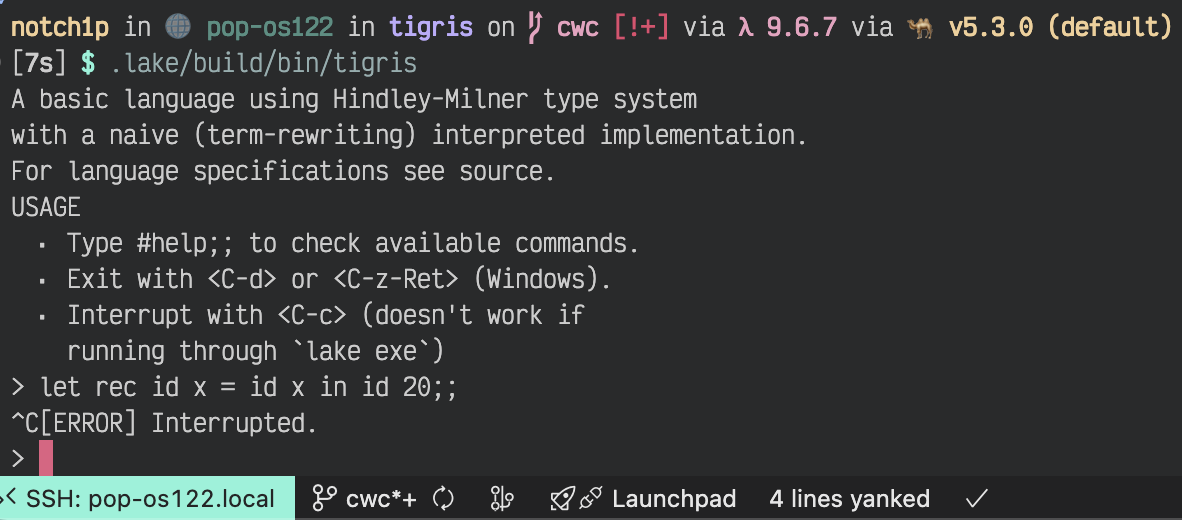
\includegraphics[width=0.5\linewidth]{assets/term1}
\caption{A user interrupting a computation}\label{img:term1}
\end{figure}

The \emph{Tigrisi} interpreter can be invoked with \texttt{interpretL} (w/o incr. APIs) or \texttt{interpretI}, of which the former is stable and is used to quickly test the lowering stage to see if there is any issue.

\subsection{CPS transformation}
\paragraph{CPS transformation} refers to the transformation of \Lambdair into its CPS counterparts where
\begin{itemize}
\item every function takes an explicit continuation parameter $k$,
\item function calls pass results to continuations rather than returning,
\item continuations are \emph{not} first-class: they are either
  locally-bound labels or the special parameter $k$,
\item ANF is maintained.
\end{itemize}
The use of CPS, as explained in the section about tailcall, is to transform non-tailrec functions.
This is rather specific as in general, mechanized CPS is used to \underline{encode complex control flow},
similar to a \texttt{longjmp} and CPS transformation is to \underline{make control flow explicit}, at the expense of
increased heap usage, as continuations are usually lambda abstraction\footnote{
which usually is allocated in heap. Though most compilers may force stack allocation
if there is an optimization window, that defeats the purpose of using CPS to save stack space if it is
too naive.
}
them selves, being passed around together
with function parameters. The intuition is that, CPS trades heap space for stack space,
by allocating and \emph{compositing} continuations, which, can be thought as
\begin{center}
\underline{an explicit call stack (that replaces the actual call stack)
which is unwinded when applied.}
\end{center}

The CPS IR is similar to \Lambdair, defined as (\texttt{CName} is \texttt{Name})
\begin{minted}[numbers=left]{lean4}
  inductive CRhs where
    | prim     (op : PrimOp) (args : Array CName)
    | proj     (src : CName) (idx : Nat)
    | mkPair   (a b : CName)
    | mkConstr (tag : Name) (fields : Array CName)
    | isConstr (src : CName) (tag : Name) (arity : Nat)
    | const    (k : Const)
    | alias    (y : CName)   -- x = y
  deriving Repr, Inhabited, BEq

  mutual
  inductive CTail where
    | appFun      (f : CName) (payload : CName) (k : CName)
    | appKont     (k : CName) (value : CName)
    | ite         (condVar : CName) (tBranch eBranch : CExpr)
    | switchConst (scrut : CName)
                  (cases : Array (Const × CExpr))
                  (default? : Option CExpr)
    | switchCtor  (scrut : CName)
                  (cases : Array (Name × Nat × CExpr))
                  (default? : Option CExpr)
    | halt        (value : CName)
    | matchFail   (pat : Array Name)
  deriving Repr, Inhabited, BEq

  /-- CPS expression in ANF: pure let1 / letKont / local fun groups, ending with a tail. -/
  inductive CExpr where
    | let1    (x : CName) (rhs : CRhs) (body : CExpr)
    | letKont (kid : CName) (param : CName) (kBody : CExpr) (body : CExpr)
    | letRec  (funs : Array CFun) (body : CExpr)
    | tail    (t : CTail)
  deriving Repr, Inhabited, BEq

  structure CFun where
    fid          : CName
    payloadParam : CName
    kontParam    : CName
    body         : CExpr
  deriving Repr, Inhabited, BEq
  end
\end{minted}

The CPS transformation is the last step of the IR lowering process, which, is further lowered by
the SBCL backend to Common Lisp. Semantics of the actual program should be similar to that of CPS,
provided if there is not any backend inconsistency\footnote{
which, unfortunately, remains an assumption because \Tigris is not formally verified. Note that, the \texttt{M} monad is continued to use for this transformation.
}

First, we present the formal grammar of \Lambdair, and its CPS target:

\begingroup\allowdisplaybreaks
\begin{align*}
v \in \Val &::= x \mid k \mid \ctor(t, \bar{x}) \mid \lambda p.\, e \\[4pt]
r \in \mathsf{Rhs} &::= \prim(\mathit{op}, \bar{x}) \mid \proj(x, i) \mid \mkpair(x, y) \\
&\mid \mkctor(t, \bar{x}) \mid \isctor(x, t, n) \mid f(a) \\[4pt]
s \in \mathsf{Stmt} &::= \letone x = r \\[4pt]
\tau \in \mathsf{Tail} &::=\mathbf{ret}\, x \mid f(a)^{\mathsf{T}}\\
&\mid \mathbf{if}\, c\, \mathbf{then}\, e_1\, \mathbf{else}\, e_2 \\
&\mid \switch^{\Const}(x, \overline{k_i \to e_i}, e_?) \\
&\mid \switch^{\ctor}(x, \overline{(t_i, n_i) \to e_i}, e_?) \\
&\mid \fail \\[4pt]
e \in \mathsf{LExpr} &::=\bar{s};\, \tau \\
&\mid \mathbf{let}_\iota\, x = v\, \mathbf{in}\, e \\
&\mid \letone x = r\, \mathbf{in}\, e \\
&\mid \letRec\, \overline{f_i(p_i) = e_i}\, \mathbf{in}\, e\\
r_c \in \mathsf{CRhs} &::=\prim(\mathit{op}, \bar{x}) \mid \proj(x, i) \mid \mkpair(x, y) \\
&\mid \mkctor(t, \bar{x}) \mid \isctor(x, t, n) \mid k \mid x \\[4pt]
\tau_c \in \mathsf{CTail} &::=f(p, k) \mid k(v) \mid \halt(v) \\
&\mid \ite(c, e_1, e_2) \\
&\mid \switch^{\Const}(x, \overline{k_i \to e_i}, e_?) \\
&\mid \switch^{\ctor}(x, \overline{(t_i, n_i) \to e_i}, e_?) \\
&\mid \fail \\[4pt]
e_c \in \mathsf{CExpr} &::=\letone x = r_c\, \mathbf{in}\, e_c \\
&\mid \letK\, \kappa(p) = e_c\, \mathbf{in}\, e_c \\
&\mid \letRec\, \overline{f_i(p_i, k_i) = e_i}\, \mathbf{in}\, e_c \\
&\mid \mathsf{tail}\, \tau_c
\end{align*}\endgroup

We define the \emph{domain of semantics} (i.e. datatypes) as:\footnote{
think of $(+)$ and $(\times)$ as coproduct and product, respectively.
}

\begin{align*}
\Val &= \unit + \mathbb{Z} + \mathbb{B} + \mathsf{String} + (\Val \times \Val) + (\Name \times \Val^*) + \Name \\
\Env &= \Name \rightharpoonup \Val \\
\FunTab &= \Name \rightharpoonup (\Name \times \Name \times \mathsf{CExpr}) \\
\KontTab &= \Name \rightharpoonup (\Name \times \mathsf{CExpr}) \\
\mathsf{Ans} &= \Val + \mathsf{Error}
\end{align*}

The transformation $\mathcal{C} :  \mathsf{LExpr} \to \mathsf{CExpr}$ is defined
with respect to a \emph{current continuation} $k$, which is either a continuation
variable or should be the identity continuation $\mathrm{id}_\mathsf{Ans}$\footnote{
The standard \emph{driver} in SBCL backend is this.
}
for top-level expressions.

Below, we present the denotational semantics for this transformation. Note that $C^k_{[\bullet]}$ represents a
a transformation with bound continuation $k$, with a hole denoting an element of the input domain $[\bullet]$, which is one of
$v, r, s, \tau, e$; And $C^k_s\sem{\bullet}(e_c)$ threads $e_c$. We simplify \texttt{let*} and \texttt{switch*} to
just one binding/one discriminant.

\begingroup
\allowdisplaybreaks
\begin{align*}
\mathcal{C}_v\sem{x} &= x \tag{Values} \\
\mathcal{C}_v\sem{k} &= \mathsf{const}(k) \\
\mathcal{C}_v\sem{\ctor(t, \bar{x})} &= \mkctor(t, \bar{x})\\
\mathcal{C}_r\sem{\prim(\mathit{op}, \bar{x})} &= \prim(\mathit{op}, \bar{x}) \tag{Rhs} \\
\mathcal{C}_r\sem{\proj(x, i)} &= \proj(x, i) \\
\mathcal{C}_r\sem{\mkpair(x, y)} &= \mkpair(x, y) \\
\mathcal{C}_r\sem{\mkctor(t, \bar{x})} &= \mkctor(t, \bar{x}) \\
\mathcal{C}_r\sem{\isctor(x, t, n)} &= \isctor(x, t, n) \\
\mathcal{C}_r\sem{f(a)} &= \text{(see call transformation below)}\\
\mathcal{C}_\tau^k\sem{\mathbf{ret}\, x} &= \mathsf{tail}\, k(x) \tag{Tails} \\[6pt]
\mathcal{C}_\tau^k\sem{f(a)^{\mathsf{T}}} &= \mathsf{tail}\, f(a, k) \\[6pt]
\mathcal{C}_\tau^k\sem{\mathbf{if}\, c\, \mathbf{then}\, e_1\, \mathbf{else}\, e_2} &=
\mathsf{tail}\, \ite(c, \mathcal{C}^k\sem{e_1}, \mathcal{C}^k\sem{e_2}) \\[6pt]
\mathcal{C}_\tau^k\sem{\switch^{\Const}(x, \overline{k_i \to e_i}, e_?)} &=
\mathsf{tail}\, \switch^{\Const}(x, \overline{k_i \to \mathcal{C}^k\sem{e_i}}, \mathcal{C}^k\sem{e_?}) \\[6pt]
\mathcal{C}_\tau^k\sem{\switch^{\ctor}(x, \overline{(t_i, n_i) \to e_i}, e_?)} &=
\mathsf{tail}\, \switch^{\ctor}(x, \overline{(t_i, n_i) \to \mathcal{C}^k\sem{e_i}}, \mathcal{C}^k\sem{e_?}) \\[6pt]
\mathcal{C}_\tau^k\sem{\fail} &= \mathsf{tail}\, \fail\\
\mathcal{C}_s^k\sem{\bar{s};\, \tau} &= \mathcal{C}_s^k\sem{\bar{s}}(\mathcal{C}_\tau^k\sem{\tau}) \tag{Stmt} \\
\mathcal{C}_s^k\sem{\epsilon}(e_c) &= e_c \\
\mathcal{C}_s^k\sem{(\letone x = r); \bar{s}}(e_c) &=
\begin{cases}
  \letK\, \kappa(x) = \mathcal{C}_s^k\sem{\bar{s}}(e_c)\, \mathbf{in}\, \mathsf{tail}\, f(a, \kappa)
  & r = f(a) \\
  \letone x = \mathcal{C}_r\sem{r}\, \mathbf{in}\, \mathcal{C}_s^k\sem{\bar{s}}(e_c)
  & \text{otherwise}
\end{cases}\\
\mathcal{C}^k\sem{\mathbf{let}_\iota\, x = v\, \mathbf{in}\, e} &=
\letone x = \mathcal{C}_v\sem{v}\, \mathbf{in}\, \mathcal{C}^k\sem{e} \tag{letVal} \\
\mathcal{C}^k\sem{\letone x = f(a)\, \mathbf{in}\, e} &=
\letK\, \kappa(x) = \mathcal{C}^k\sem{e}\, \mathbf{in}\, \mathsf{tail}\, f(a, \kappa) \tag{letRhs} \\
\mathcal{C}^k\sem{\letone x = r\, \mathbf{in}\, e} &=
\letone x = \mathcal{C}_r\sem{r}\, \mathbf{in}\, \mathcal{C}^k\sem{e}
\quad (r \neq f(a)) \\
\mathcal{C}^k\sem{\letRec\, f(p) = e_f\, \mathbf{in}\, e} &=
\letRec\, f(p, k_f) = \mathcal{C}^{k_f}\sem{e_f}\, \mathbf{in}\, \mathcal{C}^k\sem{e} \tag{letRhs} \\
\end{align*}
\endgroup

Finally, we present the denotational semantics of CPS IR \emph{itself}. Just as above, the semantics is
given by
\begin{align*}
\mathcal{E} &: (\mathsf{CExpr}\oplus\mathsf{CTail}) \to \Env \to \FunTab \to \KontTab \to (\Val \to \mathsf{Ans}) \to \mathsf{Ans}\\
\mathcal{R} &: \mathsf{CExpr}\to\Env\to\Val
\end{align*}
where the fifth parameter i.e. of type $\Val\to\Ans$ is the \emph{outermost continuation},
or the \emph{meta-continuation}, denoted $\mu$,
which represents the toplevel continuation that is $\mathrm{id}_\mathsf{Ans}$ or $\halt$.
We write $\rho[n\mapsto v]$ to denote the insertion\footnote{
insertion follows the standard behavior: if the key $m$ exists, its value is replaced by $v$.
}
of mapping $n\mapsto v$ to $\rho$; Readers should acknowledge that $\rho,n,v$ are metavariables.
Note that $\mathcal{E}$ takes both tails and expressions.

\begingroup\allowdisplaybreaks
\begin{align*}
\footnotemark\mathcal{R}\sem{\prim(\mathit{op}, \bar{x})}\Env &= \delta(\mathit{op}, \Env(\bar{x})) \tag{CRhs} \\
\mathcal{R}\sem{\proj(x, i)}\Env &= \pi_i(\Env(x)) \\
\mathcal{R}\sem{\mkpair(x, y)}\Env &= (\Env(x), \Env(y)) \\
\mathcal{R}\sem{\mkctor(t, \bar{x})}\Env &= (t, \Env(\bar{x})) \\
\mathcal{R}\sem{\isctor(x, t, n)}\Env &=
\begin{cases}
  \mathsf{true} & \Env(x) = (t, \bar{v}) \land |\bar{v}| = n \\
  \mathsf{false} & \text{otherwise}
\end{cases} \\
\mathcal{R}\sem{\mathsf{const}(k)}\Env &= k \\
\mathcal{R}\sem{\mathsf{alias}(y)}\Env &= \Env(y)\\
\mathcal{E}\sem{f(p, k)}\Env\FunTab\KontTab\mu &=
\begin{cases}
  \mathcal{E}\sem{e_f}\Env'\FunTab'\KontTab'\mu
  & \FunTab(f) = (p_f, k_f, e_f) \tag{funapp} \\
  \mathsf{Error} & \text{otherwise}
\end{cases}\\
\text{where}\quad\Env' &= \{p_f \mapsto \Env(p),\, k_f \mapsto \Env(k)\} \\
\FunTab' &= \FunTab \\
\KontTab' &= \varnothing \quad \text{(local continuations are scoped)}\\
\footnotemark\mathcal{E}\sem{\kappa(v)}\Env\FunTab\KontTab\mu &=
\begin{cases}
  \mathcal{E}\sem{e_\kappa}\Env[p_\kappa \mapsto \Env(v)]\FunTab\KontTab\mu
  & \KontTab(\kappa) = (p_\kappa, e_\kappa) \tag{kontapp} \\
  \mu(\Env(v))
  & \kappa = k_{\mathsf{param}} \\
  \mathsf{Error} & \text{otherwise}
\end{cases}\\
\mathcal{E}\sem{\halt(v)}\Env\FunTab\KontTab\mu &= \Env(v) \tag{halt}\\
\mathcal{E}\sem{\ite(c, e_1, e_2)}\Env\FunTab\KontTab\mu &=
\begin{cases}
  \mathcal{E}\sem{e_1}\Env\FunTab\KontTab\mu & \Env(c) = \mathsf{true} \tag{conditional} \\
  \mathcal{E}\sem{e_2}\Env\FunTab\KontTab\mu & \text{otherwise}
\end{cases}\\
\mathcal{E}\sem{\switch^{\Const}(x, \overline{k_i \to e_i}, e_?)}\Env\FunTab\KontTab\mu &=
\begin{cases}
  \mathcal{E}\sem{e_j}\Env\FunTab\KontTab\mu
  & \exists j.\, \Env(x) = k_j \tag{const switch} \\
  \mathcal{E}\sem{e_? }\Env\FunTab\KontTab\mu
  & \forall i.\, \Env(x) \neq k_i \land e_? \ \text{exists} \\
  \mathsf{Error} & \text{otherwise}
\end{cases}\\
\mathcal{E}\sem{\switch^{\ctor}(x, \overline{(t_i, n_i) \to e_i}, e_?)}\Env\FunTab\KontTab\mu &=
\begin{cases}
  \mathcal{E}\sem{e_j}\Env\FunTab\KontTab\mu
  & \Env(x) = (t_j, \bar{v}) \land |\bar{v}| = n_j \tag{ctor switch} \\
  \mathcal{E}\sem{e_?}\Env\FunTab\KontTab\mu
  & \text{no match}; e_?\ \text{exists} \\
  \mathsf{Error} & \text{otherwise}
\end{cases}\\
\mathcal{E}\sem{\fail}\Env\FunTab\KontTab\mu &= \texttt{MATCH-FAILURE} \tag{matchfail}\\
\mathcal{E}\sem{\letone x = r\, \mathbf{in}\, e}\Env\FunTab\KontTab\mu &=
\mathcal{E}\sem{e}\Env[x \mapsto \mathcal{R}\sem{r}\Env]\FunTab\KontTab\mu \tag{let1}\\
\footnotemark\mathcal{E}\sem{\letK\, \kappa(p) = e_\kappa\, \mathbf{in}\, e}\Env\FunTab\KontTab\mu &=
\mathcal{E}\sem{e}\Env\FunTab\KontTab[\kappa \mapsto (p, e_\kappa)]\mu \tag{letKont}\\
\mathcal{E}\sem{\letRec\, f(p, k_f) = e_f\, \mathbf{in}\, e}\Env\FunTab\KontTab\mu &=
\mathcal{E}\sem{e}\Env\FunTab[f \mapsto (p, k_f, e_f)]\KontTab\mu \tag{letRec}\\
\mathcal{E}\sem{\mathsf{tail}\, \tau}\Env\FunTab\KontTab\mu &=
\mathcal{E}\sem{\tau}\Env\FunTab\KontTab\mu \tag{tail}
\end{align*}
\endgroup

\addtocounter{footnote}{-2}
\footnotetext{where $\delta$ is the interpretation of primitive operations and $\pi_i$ is projection.}
\stepcounter{footnote}
\footnotetext{The second case handles the distinguished continuation parameter: applying it
invokes the toplevel continuation $mu$, effectively returning from the current function.}
\stepcounter{footnote}
\footnotetext{Note that continuations are \emph{not} values in the environment; they are stored
in a separate continuation table $\KontTab$, \underline{reflecting that they are not first-class.}}

Experienced readers should immediately notice some key properties based on the definition of
this CPS IR, nevertheless, we list them as remarks below:

\begin{remark}[Non-first class continuations] refer
to continuations appear only in specific syntactic positions, as listed below:
\begin{enumerate}
  \item As the second argument to function calls:  $f(p, k)$
  \item As the target of continuation application: $\kappa(v)$
  \item Bound by $\letK$: $\letK\, \kappa(p) = e\, \mathbf{in}\, \ldots$
\end{enumerate}
This is enforced by the definition (abstract syntax) of CPS IR, where there is
no \texttt{CRhs} that captures a continuation as a value. Some users might be disappointed
as such IR could not support advanced control primitives such as $\mathsf{call/cc}$ or
$\mathsf{shift}$/$\mathsf{reset}$ from delimited continuation. Although such primitives can be more
efficiently treated by the compiler, this form of CPS really is not widely used and can be substituted
for more boilerplate code. Even If one must use it,
we suggest an \emph{internalized} version \texttt{Cont} which is more local with
good maintainability\footnote{since CPS itself can be convoluted and counterintuitive of which
the incautious use is just as bad as \texttt{goto}.}
through the \texttt{Monad} interface, similar to the one from \texttt{Control.Monad.Cont} in GHC.
Refer to testcase \texttt{examples/cont.tig} for an example.
\end{remark}

\begin{remark}[Guaranteed tailcall] refers to the fact that all function calls in CPS are in tail position.
\[
  \mathcal{E}\sem{f(p, k)}\ldots\ \text{directly invokes}\ f\ \text{without building stack frames}
\]
Non-tail calls in the source are transformed via $\letK$:
\[
  \letone x = f(a)\, \mathbf{in}\, e
  \quad\leadsto\quad
  \letK\, \kappa(x) = \mathcal{C}^k\sem{e}\, \mathbf{in}\, \mathsf{tail}\, f(a, \kappa)
\]
where the continuation $\kappa$ captures the \underline{rest of the computation} $e$.
\end{remark}

\begin{remark}[Closure representation after CPS]
Previously, we discussed the encoding and calling convention of function objects, this, is
largely unchanged after CPS:
\[
  \mathbf{C}\llbracket \mathit{ptr}, \Gamma \rrbracket
\]
where $\Gamma$ is the captured environment.  In CPS, function calls become:
\[
  \mathcal{E}\sem{f(p, k)} = \ldots\ \text{where}\ f\ \text{is a code pointer}
\]
The payload $p$ is a pair $(\alpha, \Gamma)$ where $\alpha$ contains the user arguments.
\end{remark}

\begin{remark}[CPS Module semantics]
A CPS module consists of:
\begin{align*}
  M &= (\bar{F}, F_{\mathit{main}}) \\
  F &= (f, p, k, e)
\end{align*}

The semantics of a module is:
\[
  \mathcal{M}\sem{(\bar{F}, F_{\mathit{main}})} =
  \mathcal{E}\sem{e_{\mathit{main}}}\Env_0\FunTab_0\varnothing\,\mathrm{id}_\mathsf{Ans}
\]
where:
\begin{align*}
  \FunTab_0 &= \{f_i \mapsto (p_i, k_i, e_i) \mid F_i\ \mathbf{of}\ (f_i, p_i, k_i, \cdot) \in \bar{F}\} \cup \{f_{\mathit{main}} \mapsto (p_m, k_m, e_m)\} \\
  \Env_0 &= \{p_m \mapsto (\unit, \mathbf{E}\llbracket\rrbracket)\}
\end{align*}

The initial payload is $(((), ()), \mathbf{E}\llbracket\rrbracket)$\footnote{
  Recall, for function with parameter $a$ of arity 1, we construct $(a, ())$ even if
  $a = ()$.
}. Though, this behavior can be changed in the backend by modifying the driver wrapper code to pass
whatever value to \texttt{main} in Common Lisp.
\end{remark}

\subsection{Backend: Common Lisp (SBCL) \& FFI}\label{sect:ffi}
Before proceeding further, let us recap all the stages in the implementation of Tigris, through datatypes:

\begin{align*}
\text{\Tigris source}&
\xrightarrow{\text{\textcircled{\tiny 1}}}\mathsf{Expr}
\xrightarrow{\text{\textcircled{\tiny 2}}}\mathsf{TExpr}
\xrightarrow{\text{\textcircled{\tiny 3}}}\mathsf{FExpr}
\xrightarrow{\text{\textcircled{\tiny 4}}}\mathsf{LExpr}
\xrightarrow{\text{\textcircled{\tiny 5}}}\mathsf{CExpr}
\xrightarrow{\text{\textcircled{\tiny 6}}}\text{LISP source}\\
\text{where}\
&\text{\textcircled{\footnotesize 1}}:\text{lexing, parsing}
\quad\text{\textcircled{\footnotesize 2}}:\text{typechecking}
\quad\text{\textcircled{\footnotesize 3}}:\text{instance resolution, SysF elaboration}\\
&\text{\textcircled{\footnotesize 4}}:\text{\Lambdair lowering}
\quad\text{\textcircled{\footnotesize 5}}:\text{CPS conversion}
\quad\text{\textcircled{\footnotesize 6}}:\text{SBCL codegen}
\end{align*}

\paragraph{The SBCL backend} simply translate CPS IR to Common Lisp source.
Since SBCL is functional and dynamically typed, specialization or most type information is not needed,
continuations are created as-is and
\emph{defunctionalization} is not attempted.
The reason
for choosing Common Lisp
instead of other languages such as JS or Go is because the author considers himself a LISPer,
who enjoys using macros.

Informally, we describe the translation as follows:
\subparagraph*{toplevel functions} refer to all functions, of shape $fid(pl, k)$, as
\mintinline{lisp}|(defun fid (pl k))|;
\subparagraph*{let-binding} i.e. \texttt{let1} as the standard \mintinline{lisp}|(let ((n v)) ..)|;
\subparagraph*{kont-binding} i.e. \texttt{letKont k v = ..} is translated to \mintinline{lisp}{(labels ((k (v) ..)) body)};
\subparagraph*{kont-app} i.e. \texttt{APPLY k v} as \mintinline{lisp}|(funcall (the function k) v)|
\subparagraph*{closure} i.e. $\mathbf{C}\sem{ptr, \Gamma}$ as \mintinline{lisp}|#'ptr| if $ptr$ is
toplevel/label-bound, or otherwise, store as-is;
\subparagraph*{$\Gamma$} i.e. $\mathbf{E}\sem{\bar{f}}$, for each field $f$,
\begin{itemize}
\item store as-is if $f$ is a local functional value,
  \item store \mintinline{lisp}|#'f| if $f$ is toplevel/label-bound,
\item store as-is, otherwise.
\end{itemize}
\subparagraph*{funcall} i.e. $f(a, k)$ as \mintinline{lisp}|(funcall (the function f) ..)| where $f$ is local, or \mintinline{lisp}|(funcall #'f ..)| where $f$ is toplevel/label-bound
\subparagraph*{conditionals} i.e. $\ite(c,t,e)$ as \mintinline{lisp}|(if c t e)|
\subparagraph*{switch} where
\begin{itemize}
\item $\switch^{\Const}(x, \overline{k_i \to e_i}, e_?)$ as
  \mintinline{lisp}|(cond (((equal x k_i) e_i) .. (t e_?)) ..)|
\item $\switch^{\ctor}(x, \overline{(t_i, n_i) \to e_i}, e_?)$
  \mintinline{lisp}|(cond (((eq x t_i) e_i) .. (t e_?)) ..)|
\end{itemize}
\subparagraph*{product} i.e. $pr = (p, q)$ to \mintinline{lisp}|(cons p q)|
and projects with the standard \mintinline{lisp}|(car pp)| or \mintinline{lisp}|(cdr pp)|
\subparagraph*{variant} i.e. $ctag\sem{\overline{fld}}$ as \mintinline{lisp}|(cons tag (vector @fld))|\footnote{
as in \mintinline{lisp}|'simple-vector|, the fastest stock array variant. Note that \texttt{@x} denotes
the splice of x.
}
with projection $x_i$ as \mintinline{lisp}|(svref (cdr x) i)|. $\mathbf{E}$ and $\mathbf{C}$ are encoded
this way as well.
\subparagraph*{test-ctor} i.e. $\isctor(x, tag, \dot)$ as \mintinline{lisp}|(eq (car x) tag)|. Note that
arity is \underline{not} checked at this time.
\emph{Symbols} appear inside CPS IR are escaped with bars \texttt{||} to preserve the case, as in
\begin{minted}{lean4}
  def sym (s : Name) : String :=
    let esc := s.foldl (init := "|") fun acc ch =>
      match ch with
      | '|' => acc ++ "\\|"
      | '\\' => acc ++ "\\\\"
      | _ => acc.push ch
    esc.push '|'
\end{minted}
The caveats, as described in \autoref{sbcl:cav} (uncurrying), because type information is erased, we
collect \emph{shapes} on demand to \emph{alleviate} this problem, where \texttt{Shapes} can be thought as degenerate types
\begin{minted}{lean4}
  inductive Shape where
    | unknown
    | pair
    | ctor (tag : Name) (arity : Nat)
    | fn -- function object inside value cell
  deriving Inhabited, BEq, Repr
abbrev ShapeEnv := Std.HashMap Name Shape
\end{minted}
where \texttt{ShapeEnv} associates a name with a shape.
The initial shape of a name is always \texttt{unknown},
but will be \emph{refined} as the code is being compiled.
However we use the word \emph{alleviate} because this method is \underline{not robust} as it it local to functions and does not deal with the root cause: design flaws.
Major refactor of adding type information to Lambda IR, threading through CPS transformation and
codegen must be made to address the issue.

\paragraph{The runtime system} refers to the primitive operator implementations, driver code and
the definitions of low-level exceptions, e.g. the string equality \texttt{\%string=}
, the integer addition \texttt{\%int+} and the \texttt{MATCH-FAILURE} condition \texttt{+NOMATCH+}\footnote{
Common Lisp have \emph{conditions}, which, is arguably more expressive and general then
other languages' exception system as it encodes all kinds of control flow, not just exceptions.
In fact, it can be
used to implement an internalized continuation facility.
}
is implemented as
\begin{minted}[numbers=left]{lisp}
  (declaim (inline %string=))
  (defun %string= (s1 s2)
    (declare (type simple-string s1 s2))
    (the boolean (sb-kernel:%sp-string= s1 s2 0 nil 0 nil)))

  (declaim (ftype (function (integer integer) integer) %int+) (inline %int+))
  (defun %int+ (a b)
    (declare (optimize (speed 3) (debug 0) (safety 0)))
    (sb-kernel:two-arg-+ a b))

  (define-condition match-failure (error)
    ((discriminant :initarg :discr :reader discriminant :type string))
    (:report
     (lambda (condition stream)
       (format stream "No branch can be matched against ~A" (discriminant condition)))))
  (defconstant +NOMATCH+ 'match-failure)
\end{minted}
Interested readers should refer to \texttt{runtime.lisp}.

Common Lisp have all kinds of equality relations. To minimize overhead on dynamically typed languages, we largely follow \autoref{tab:lisp-eq}.
\texttt{EQ} is the most efficient as it compares memory address
(i.e. physical equality rather than structural equality), which,
is used most, in our case,
such as comparing constructors as they are always unique, which has the same memory address.
Compared to the usual encoding of constructors as integers, we achieve same performance here with
better readability since the name of the constructor is the symbol itself.

\begin{table}[]
\centering
\begin{tabular}{@{}ll@{}}
  \toprule
  \textbf{To compare against..} & \textbf{Use..}                               \\ \midrule
  Objects/Structs               & \texttt{EQ}                                         \\
  Symbols                       & \texttt{EQ}                                         \\
  NIL                           & \texttt{EQ/NULL}                                  \\
  T                             & \texttt{EQ}                                         \\
  Precise numbers               & \texttt{EQL}                                        \\
  Floats                        & \texttt{=}                                          \\
  Char                          & \texttt{EQL/CHAR=}                                \\
  List/Cons/Seq                 & \texttt{EQUAL}                                      \\
  String                        & \texttt{EQUAL/EQUALP/STRING=} (symbols as well) \\
  Tree                          & \texttt{TREE-EQUAL}                                 \\ \bottomrule
\end{tabular}
\caption{LISP equalities}\label{tab:lisp-eq}
\end{table}

\begin{remark}[Inlining runtime]
The content of \texttt{runtime.lisp} is \emph{inlined} in the compiler, through a trick
used in the build script (also in Lean.) which detects whether there is a change in the file, and
writes to \texttt{runtime.lean} if so:

\begin{Verbatim}[numbers=left]
  input_file runtime.lisp where
    path := __dir__ / "runtime.lisp"
    text := true
  target runtime.lean : Unit := do -- NOTE: see also `meta` (modifier)
    let runtimep <- runtime.lisp.fetch
    let rstrBegin := "r###\"\n".toUTF8
    let rstrEnd   := "\"###".toUTF8
    runtimep.mapM fun path =>
      IO.FS.withFile path .read fun rt =>
        IO.FS.withFile (__dir__ / "runtime.lean") .write fun h => do
          let runtime <- rt.readBinToEndInto rstrBegin
          h.putStrLn s!"/-- generated from {path} -/"
          h.putStrLn "def runtime : String :="
          h.write $ runtime.pushMany rstrEnd
\end{Verbatim}
\end{remark}

\paragraph{FFI} or \emph{foreign function interface}, refers to calling functions external to the language.
Since \Tigris compiles to SBCL, a rather high and low-level\footnote{
Common Lisp is high-level in having GC and being a dynamically typed functional language;
and is low-level in having basic special operators and a bunch of low-level features such as
\mintinline{lisp}{go}, \mintinline{lisp}{block}, \mintinline{lisp}{progn} that
dates back to 1950s.
}
language, FFI is obtained for \emph{free} if one is familiar with the calling convention
described before as we do not have to deal with memory management or boxing/unboxing.
Metaprogramming is used extensively
to make the use of FFI as convenient as possible.
Since \Tigris is not able to see an externally defined function, it
puts every trust it has in the user whom is responsible for
\begin{center}\underline{making sure the function is correctly typed,
both in LISP and in the \texttt{extern} declaration.}
\end{center}

However, schemes declared this way can not be checked for their \emph{sanity}, i.e.,
it is possible to \underline{inhabit the types that should otherwise be empty},
or types that can only be proved (inhabited) with circular argument such as
$\forall\alpha.\;\alpha$ or $\forall\alpha,\beta.\;\alpha\to\beta$. Though, the former
already exists because of the deprecated fixpoint combinator \texttt{rec}, as in $\mathsf{rec}\ \mathrm{id}_\alpha$,\footnote{
while it damages the soundness of the type system, we keep it nonetheless for educational
purposes. Besides, users can avoid it, since normal programming do not use \texttt{rec} at all.
}
whereas the latter could be useful, though unsafely, when specialized
to $\forall\alpha.\;\mathsf{Unit}\to\alpha$ (as seen in an example later).

We illustrate the use of FFI through a somewhat elaborate example:

\begin{minted}{lean4}
  extern println "%println" : forall a, a -> Unit
  extern append "%string-append" : String -> String -> String
  extern toString "%to-string" : forall a, a -> String
  extern read "%read" : forall a, Unit -> a
  infixl 65 "++" => append

  let fact n =
    let rec go acc
      | 0 => acc
      | m =>
        let _ = println $ "fact "
                       ++ toString (n - m) ++ " = "
                       ++ toString (acc * m)
        in go an @@ m - 1
    in go 1 n
  postfix 50 "!" => fact

  let main =
    let _ = println "Enter a number:" in
    let x = read () in
    x ! -- x! is also a valid identifier. So we parenthesize it/use juxtaposition.
\end{minted}

\texttt{read} is an unsafe function whose return type can be specialized to any type,
in this case, \texttt{Int}.
Internally, a name associated to a FFI declaration is transformed, during parsing, to its
FFI name, e.g., \texttt{read} becomes \texttt{\%read}. Where the implementations of these
external functions are

\begin{minted}{lisp}
(defforeign |%to-string| (x _) ;; e.g. toString : ∀a, a -> String
  (declare (ignore gamma _))
  (funcall k (princ-to-string x)))
(defforeign "%string-append" (x y) ;; e.g. string-append : String -> String -> String
  (declare (ignore gamma) (type string x y))
  (funcall k (concatenate 'string x y)))
(defforeign |%read| (_ __) ;; e.g. read (unsafe) : ∀a, Unit -> a
  (declare (ignore gamma _ __))
  (funcall k (read)))
(defforeign |%println| (x _) ;; e.g. println : ∀a, a -> Unit
  (declare (ignore gamma _))
  (princ x) (terpri)
  (funcall k nil))
\end{minted}

Compiling and running the program results in\footnote{though
\texttt{ffi.lisp} in this case in automatically linked. Linking it again with \texttt{--link} would
make SBCL complain about duplicate definitions. \texttt{--link} here is only to demonstrate its use.
}

\begin{Verbatim}[numbers=left]
  $ tigrisl examples/fact.tig --link ffi.lisp -o dist-fact.fasl && chmod +x dist-fact.fasl
  ; wrote (...)/dist-fact.fasl
  ; compilation finished in 0:00:00.021
  $ ./dist-fact.fasl
  Enter a number:
  > 5
  fact 0 = 5
  fact 1 = 20
  fact 2 = 60
  fact 3 = 120
  fact 4 = 120
  120
\end{Verbatim}

For users with LISP experience, they will quickly notice the unfamiliar notation \texttt{defforeign}.
This, together with other gadgets,
are LISP macros to make the definition of foreign
functions easier, which lives inside \texttt{ffi.lisp}. Amongst them, the most important are
\begin{itemize}
\item \texttt{WITH-ARGS} destructures \texttt{payload = (cons α Γ)} and binds each user argument
  to the symbols provided and a special variable \texttt{GAMMA} denoting the captured environment. Basically,
  it generates the prelude part of a function where payload are destructured according to the provided
  \emph{lambda list}\footnote{LISP jargon. Refers to s list that specifies a set of parameters (sometimes called lambda variables) and a protocol for receiving values for those parameters.}.
  This macro is not supposed to be used along; It is intended to be called by
  \texttt{defforeign} and users should use that instead.
  \texttt{with-args} is defined as
  \begin{minted}[numbers=left]{lisp}
    (defmacro with-args (payload arg-list &body body)
      (let* ((alpha (gensym "ALPHA"))
             (tmp   (gensym "TMP")))
        (labels ((build-binds (args)
                              (cond
                               ((null args) '())
                               ((null (cdr args)) `((,(car args) (car ,tmp))))
                               (t
                                 (let ((head (car args))
                                       (rest (cdr args)))
                                   (append `((,head (car ,tmp))
                                             (,tmp  (cdr ,tmp)))
                                     (if (null (cdr rest))
                                         `((,(car rest) ,tmp))
                                         (build-binds rest))))))))
          `(let* ((,alpha (car ,payload))
                  (gamma  (cdr ,payload))
                  (,tmp   ,alpha)
                  ,@(build-binds arg-list))
             (declare (ignorable gamma))
             ,@body))))
  \end{minted}
\item \texttt{DEFFOREIGN} defines a tigris-callable foreign function. It is modeled
  after \mintinline{lisp}{defun} and combines \mintinline{lisp}{defparameter}/\texttt{with-args}.
  A foreign function definition takes the form of\footnote{
    Here we use the same BNF syntax from X3J13/CLtL2. Unexperienced users may interpret it as:
    \mintinline{lisp}|(defforeign function-name (x y) forms)| that returns a closure object,
    where \texttt{(x y)} is \texttt{ffi-lambda-list} representing
    function parameters that may vary in length;
    \texttt{forms} refers to a list of forms
    that is the function body.
  }
  \[
    \mathbf{defforeign}\ \textit{function-name}\ \textit{ffi-lambda-list}\ \{\textit{form}\}^*\longrightarrow \textit{closure-object}
  \]
  Aside from \texttt{GAMMA}, it additionally binds \texttt{k} i.e. the continuation,
  applying \texttt{k} can be thought as returning the value of the function as this is the canonical way to do so.
  \texttt{function-name}, or \texttt{name} in the implementation below, is the name of the foreign function, can be a string \texttt{"\%println"} (preserves case), or a symbol \texttt{|\%println|}.
  Users are highly recommended to escape the symbol (to preserve cases)
  as LISP by default does not distinguish cases but
  \Tigris does.
  \texttt{defforeign} is implemented as
  \begin{minted}[numbers=left,escapeinside=\%\%]{lisp}
    (defmacro defforeign (name arg-list &body body)
      (flet ((name-to-string (x)
                               (etypecase x
                                 (string x)
                                 (symbol (symbol-name x))))
             (escape-bar (s)
                         (with-output-to-string (out)
                           (loop for c across s do
                                   (case c
                                     (#\| (write-string "\\|" out))
                                     (#\\ (write-string "\\\\" out))
                                     (t (write-char c out))))))
             (make-closure (f)
                           `(cons %$\mathbf{C}$% (vector
                                       (function ,f)
                                       (cons %$\mathbf{E}$% (vector))))))
        (let* ((ns     (name-to-string name))
               (fn-sym (intern (escape-bar ns)))
               (cell   (intern ns))
               (clos   (make-closure fn-sym)))
          `(eval-when (:compile-toplevel :load-toplevel :execute)
             (defun ,fn-sym (payload k)
               (with-args payload ,arg-list ,@body))
             (defparameter ,cell ,clos)))))
  \end{minted}
  Note that the use of special operator \mintinline{lisp}|eval-when| is to make sure that any
  foreign functions defined in this way gets compiled and bound when \mintinline{lisp}|(load ..)|.
\end{itemize}

With these macros, defining foreign functions should be as easy as defining normal LISP functions.

\subparagraph*{caution!} Any function output by the SBCL backend has the following compiler instructions:
  \begin{minted}{lisp}
    (declare (optimize (speed 3) (safety 0) (debug 0)))
  \end{minted}
which removes most safety features of LISP, maximizing performance.
Any error can result in a compromised LISP image (memory environment) with
unreadable low-level error messages. It is best to remove this instruction when debugging.

\paragraph{\texttt{tigrisl}} is the CLI interface to interact with the compiler.
\texttt{tigrisl} uses a simple hand-written recursive descent parser to parse command line arguments;
Multiple input files are compiled in parallel with the same amount of threads launched.
An invocation takes the form of
\[
\texttt{tigrisl}\ [\textit{flags}]\ \textit{ifiles}\ [\textsf{-o}\ \textit{ofiles}]
\]

where \textit{ifiles} and \textit{ofiles} refers to a list of input and output files that should either
\begin{itemize}
\item matches one to one. As in,
  for all $i$, input file name $f^\mathsf{in}_i$,
  there always exists a output file name $f^\mathsf{out}_i$, vice versa.
\item matches one to one, with residual \textit{ifiles}. As in,
  for \textit{ifiles}
  $f^\mathsf{in}_1,\dots,f^\mathsf{in}_i,f^\mathsf{in}_{i+1},\dots,f^\mathsf{in}_{n}$ and
  \textit{ofiles} $f^\mathsf{out}_1,\dots,f^\mathsf{out}_i$,
  we have $f^\mathsf{in}_1,\dots,f^\mathsf{in}_i$
  matching $f^\mathsf{out}_1,\dots,f^\mathsf{out}_i$,
  with residual \textit{ifiles} $f^\mathsf{in}_{i+1},f^\mathsf{in}_{n}$ using default
  output naming convention i.e. appending with \texttt{.lisp}.
\item any other situation results in a exception.
\end{itemize}
...and \underline{notable} \textit{flags} are
\begin{itemize}\itemsep0em
\item \texttt{--lam}, emit raw \Lambdair with optimizations;
\item \texttt{--cc}, emit CC'd \Lambdair;
\item \texttt{--cps}, emit CPS IR;
\item \texttt{--sysf}, emit System F IR; These four flags can be used together.
\item \texttt{-nl, --no-lisp}, do not emit Common Lisp source.
\item \texttt{-ne, --no-entry}, do not generate entrypoint, where entrypoint is also
  called driver code, that is the following:
    \begin{minted}{lisp}
      (defun |__start| ()
        (format nil "~A"
          (funcall #'|main| nil #'identity)))
    \end{minted}
\item \texttt{--legacy}, use deprecated typechecker/IR/backend. Not recommended;
\item \texttt{-l, --link <path>}, link additional lisp source from <path>, can be used multiple times. Default behavior: link \texttt{ffi.lean}. Note that, internally, linking
  a file $f$ adds a \mintinline{lisp}|(load f)| to the top of the object code. The order of
  multiple \texttt{--link}s is preserved here.
\item \texttt{-o <ofiles>}, \emph{positional vararg}, anything beyond this point is considered a part of \texttt{-o}.
  \texttt{<ofiles>} has file extension-directed output where \texttt{*.fasl} generate FASL executables and anything else for LISP sources. FASL generation is done by concatenating
  every linked LISP files together with the generated object code, then feed them into
  the launched SBCL with \emph{block compilation} on to generate a monolithic binary.
  This binary can usually run directly in shell. If that is not the case, users may
  also use \texttt{sbcl --script <fasl>} to run fasl files.
\item \texttt{--fasl}, emit FASL, applies to all input files.
\end{itemize}

\section{PP: The \emph{dependently-typed} table printer}
What's the fun when there is \Tigrisd, the theorem prover counterpart of \Tigris, but
the implementation of them doesn't involve some dependent type practices -- Actually,
both CLI interfaces and REPLs use a dependently-typed table printer that lives inside
the \texttt{PP} module, not to mention the termination proofs of some recursive functions.

The author, and this project advocates for the use of dependent types in programming and
below, we'll discuss
the design and implementation of this simple printer, hopefully, to provide
some insights into how dependent types can help users
catch more unexpected errors at compile-time,
rather than runtime.

We wish the types of table are distinguished by their headers, say, the header (name, gender, age)
should be different from (product name, manufacturer, serial number, price).
To achieve this at compile-time, we shall rely on the typechecker.
Suppose the header is a list, we may turn it into a \emph{dynamically-sized}\footnote{
In the sense that its size depends on the length of the header.
}
product \emph{type} whose length
and component type must match for the product types to be unified (Text.SString is stylized string):
\begin{minted}{lean4}
  abbrev ToProd (as : List α) (motive : Type -> Type) : Type :=
    match as with
    | [] => PUnit
    | [_] => motive α
    | _ :: x :: xs =>
      motive α × ToProd (x :: xs) motive

variable (header : List Text.SString)
abbrev Row := ToProd header id
\end{minted}

The above reads: $\mathsf{ToProd}\ (as : \mathsf{List}\ \alpha)\ f$ can be eliminated to one of 1) $\mathsf{PUnit}$\footnote{
\emph{universe-polymorphic} version of $\mathsf{Unit}$. Though since the result lives
in $\mathsf{Type}\equiv\mathsf{Type}\ 0\equiv\mathsf{Sort}\ 1$, it is effectively $\mathsf{Unit}$.
}, 2) $f\ \alpha$, or 3) $f\ \alpha \times \mathsf{ToProd}\ (\mathsf{cdr}\ as)\ f$,
based on the \emph{shape} of $as$:
\begin{enumerate}
\item where $as$ is empty;
\item where $as$ is a \emph{singleton};
\item where $as$ contains \emph{two or more} elements.
\end{enumerate}
This effectively tells us that $\mathsf{ToProd}$ can
\emph{eliminate} to one of the three\footnote{
To be precise, it is $2 + n$ for $as$ of length $n$.
} types depending on the value of $as$, specifically, its shape.
Readers should pay great attention to this approach, or thought process, as the
pattern matching used here is interpreted differently\footnote{different than a \emph{operational} interpretation, in the sense of regular programming.}
(more of a \emph{recursor}-based interpretation),\footnote{
And it is indeed in the form of recursor invocations inside the Lean \emph{kernel}.
}
which is mirrored later.

Note that \emph{motive} is type theory jargon.
It represents the target type (or a part of it) we want it to be eliminated to. Informally,
it can be best compared to the function used when mapping some data structures. Also, the
use of \mintinline{lean4}{abbrev} rather than \mintinline{lean4}{def} here guarantees the
definition to be \emph{reducible}, not \emph{semireducible} or \emph{irreducible}, allowing
the automatic unfolding of the definition when using tactics such as \texttt{rfl}, short for
reflexivity.

Now, we may encode an entry (a \texttt{Row}) of a table as \texttt{ToProd header id}. This way,
we require the entry of some table to match the shape of its header, otherwise it is
a type error; And the table type itself, obviously, can be defined as
\begin{minted}{lean4}
  abbrev TableOf := Array $ Row header
\end{minted}

We use \texttt{Array} here because it is overridden in the runtime with \emph{real continuous
data structures} rather than a linked list \texttt{List}. Besides, it also makes sense as we want
\emph{the shape} of the entry to match its header, but there should not be any size restriction
when it comes to the size of a table, i.e. the numbers of entry a table has.

Furthermore, since we are making a \emph{printer}, we want the output to look good, or at least,
looks like a table. Here we define
\begin{minted}{lean4}
  inductive Alignment | left | center | right
  inductive PadsBy | perCell | perCol
  abbrev Align := ToProd header λ _ => Alignment
  abbrev OverrideWidth := ToProd header λ _ => Option Nat
\end{minted}

where
\begin{itemize}\itemsep0em
\item \texttt{Align} is a tuple of the same shape as a header, denoting each column's alignment;
\item \texttt{PadsBy} is the padding strategy. \texttt{perCell} makes every cell
to have the same size as the largest one in them. This is rarely useful, but may look good
if the table isn't too large; \texttt{perCol} is the one that is actually useful and more familiar to users since it applies the same strategy but \underline{local to each column}.
\item \texttt{OverrideWidth}, despite its name, stores the calculated width of each column.
It is named \texttt{OverrideWidth} because it can be
overridden (\emph{before} the calculation) to have more manual
control over the output, providing better granularity.
\end{itemize}

Based on this, we sketch the configuration of this printer as

\begin{minted}{lean4}
  structure PPSpec (header : List Text.SString) where
    align    : Align header
    width    : OverrideWidth header := 0
    header?  : Bool := true
    margin   : Nat := 3
    padsBy   : PadsBy := .perCol
    truncate : Bool := false
\end{minted}
where \texttt{margin} is \emph{sum} of a cell's left and right margin. And \texttt{truncate},
which is a flag that toggles the skip of a cell if it is empty i.e. gets replaced by the cell to its right (also respects \texttt{margin});
Despite its simple nature, this is actually more interesting than one might imagine, as this could be
used to create indentation, together with margin, to achieve some interesting effects, such as
simulating tool tips, which is most useful when
printing command helppages as shown in \autoref{pp:comp}.
\begin{figure}\centering
\begin{subfigure}{0.45\textwidth}\centering
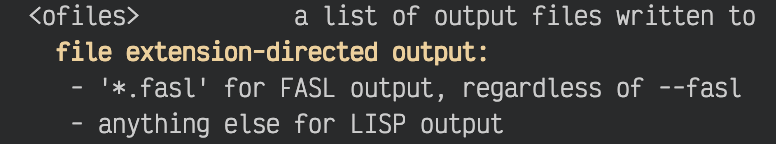
\includegraphics[width=\textwidth]{assets/term2}
\end{subfigure}%
\begin{subfigure}{0.75\textwidth}\centering
    \begin{minted}{lean4}
  (.str "<ofiles>", .str "a list of output files written to")
  (.str "", .byl "file extension-directed output:")
  (.str "", .str " - '*.fasl' for FASL output, regardless of --fasl")
  (.str "", .str " - anything else for LISP output")
    \end{minted}
\end{subfigure}
\caption{output of the table printer and its equivalent table entry}\label{pp:comp}
\end{figure}

Now, we can actually implement this printer by first
defining some helper functions that calculates the width of every column: \autoref{code:pp-col}.
This is where the aforementioned thought process come into use. The type \texttt{ToProd},
can somewhat be interpreted as having multiple values (though this ``value'' are \emph{types}),
as it \emph{depends} on its \texttt{List} argument, though, it remains as one type at a moment because
it is statically typed. We illustrate the usage of this thought process by introducing a concept called
\emph{discriminant refinement}.

Discriminant refinement is, a jargon, though fairly straightforward,
stating that the type information of a match discriminant can be \underline{\emph{refined} based on the pattern}
matching against it. An example being \mintinline{lean4}{match x with | 0 => ...}\footnote{
Though, in non-dependent type context, this feature may need to be enabled manually, in the form of
\mintinline{lean4}{match h : x with ..}, by prefixing \texttt{x} with a name \texttt{h},
for binding the hypotheses in each branch
in order to for them be picked up by the typechecker.
},
where Lean knows
that within this branch, \underline{\texttt{x} must be 0}, or as a \emph{hypothesis} that becomes
part of the \emph{ambient types}: $h : x = 0$. -- A very reasonable, and true take. This technique,
is used fairly a lot in programming with dependent types, as is in this case: we \emph{guide} Lean
the underlying type of \texttt{ToProd} through patterns against \texttt{header}:
\begin{enumerate}
\item a \texttt{[]}, stating $\textit{header} = []$, refines \texttt{ToProd} to $\mathsf{PUnit}$,
as stated in its definition;
\item a \texttt{[\_]}, stating $\textit{header} = [\cdot]$, a singleton, or, a \texttt{List} with one element of type $\alpha$, refines \texttt{ToProd} to $f \alpha$,
as stated in its definition;
\item an Erlang-like \texttt{\%[\_, \_ | \_]}, which is syntactic sugar for \texttt{\_ :: \_ :: \_}, stating
$\textit{header} = \cdot :: (\cdot :: \cdot)$, a list with two or more elements, refines \texttt{ToProd} to
a dynamically-sized product.
\end{enumerate}
Where $f$ is the motive, in this case, the constant function that maps all types to \texttt{Option Nat}.
The point of these seemingly useless patterns
differs from the regular purpose of providing templates for destructuring; Instead, it is to
provide additional information to the typechecker, which,
if not omitted, results in a type error as Lean cannot deduce the type of \texttt{header} on its own.
It is the user's responsibility to do case-by-case analysis just as in proofs. From the outsider's
perspective, it is as simple as to \underline{mirror the cases in the type definition}.

\begin{remark}[Common usage of discriminant refinement]
Furthermore, discriminant refinement deals with surrounding environment.
\texttt{foldr1} on \texttt{List} usually does not permit empty lists,
applying to such is a runtime error in Haskell, for example. In Lean, we simply make
this requirement an assumption and defines the function as:
\begin{minted}{lean4}
  def foldr1 (f : α -> α -> α) (as : List α) (h : as ≠ []) : α :=
    match as with
    | [] => h rfl |>.elim -- or simply remove this branch.
    | [x] => x
    | x :: y :: xs => f x (foldr1 f (y :: xs) nofun)
\end{minted}
where $h$ is refined to $[]\neq[]$ in the empty branch where we manually \emph{proved false} and used
\emph{ex falso} to match the expected type. Though, this branch can simply be removed as Lean can automatically
proves it \texttt{false}. Similiarly \texttt{nofun} is a shorthand used here to prove $y :: xs \neq []$, but the
proof itself automatically handled by Lean. Users calling this function must prove that $as$ is nonempty through
actual proofs or simply introducing a hypothesis using \mintinline{lean4}|if h : as ≠ [] then ..|. Though, we
shall stop here as this is beyond the scope of this text, which is not a tutorial.
\end{remark}

Getting back to implementing table printer, we found ourself having several polymorphic helpers in the sense
that they are independent of \texttt{header} and we may use it to implement some operations like \texttt{toString},
$(\cdot\;\cup\;\cdot)$, max and $0$ where it denotes the zero element of some algebraic structure. From there,
implementing printers becomes trivial.

\begin{figure}
\centering
\begin{subfigure}{0.55\textwidth}\centering
\begin{minted}{lean4}
def ovTostr (ov : OverrideWidth header)
  : String := match header with
  | [] => "" | [_] => toString ov
  | %[_, _ | _] => toString ov.1 ++ ovTostr ov.2
\end{minted}
\end{subfigure}%
\begin{subfigure}{0.55\textwidth}\centering
\begin{minted}{lean4}
def zeroOverride (header : List Text.SString)
  : OverrideWidth header := match header with
  | [] => () | [_] => none
  | %[_, y | ys] => (none, zeroOverride (y :: ys))
\end{minted}
\end{subfigure}\vspace{1em}
\begin{subfigure}{0.55\textwidth}\centering
\begin{minted}{lean4}
def maxN (h₁ h₂ : OverrideWidth header)
  : OverrideWidth header := match header with
  | [] => () | [_] => max h₁ h₂
  | %[_, _ | _] => (max h₁.1 h₂.1, maxN h₁.2 h₂.2)
\end{minted}
\end{subfigure}%
\begin{subfigure}{0.55\textwidth}\centering
\begin{minted}{lean4}
def merge (h₁ h₂ : OverrideWidth header)
  : OverrideWidth header := match header with
  | [] => () | [_] => max h₁ h₂
  | %[_, _ | _] => (h₂.1 <|> h₁.1, merge h₁.2 h₂.2)
\end{minted}
\end{subfigure}\vspace{1em}
\begin{subfigure}{\textwidth}\centering
\begin{minted}{lean4}
instance : ToString $ OverrideWidth header := ⟨ovTostr⟩
instance : Union    $ OverrideWidth header := ⟨merge⟩
instance : Max      $ OverrideWidth header := ⟨maxN⟩
instance : Zero     $ OverrideWidth header := ⟨zeroOverride header⟩
\end{minted}
\end{subfigure}
\caption{Helper functions used to calculate column width}\label{code:pp-col}
\end{figure}

\vspace{1cm}

\begin{center}
\underline{This concludes the description of \Tigris}.
\end{center}
\pagebreak

\section{\Tigrisd: a lightweight theorem prover}
\renewottcommands[dd]

\Tigrisd is a experimental dependently-typed theorem prover that demonstrates
clear, modular and exemplary theorem prover design. \Tigrisd, together with \Tigris,
is a bundled solution serving educational purposes that hopes to become useful in
\underline{programming language/theorem proving education}. \Tigrisd is deeply influenced and takes much inspiration in terms
of design/implementation from \href{https://github.com/sweirich/pi-forall}{pi-forall}\footnote{\url{https://github.com/sweirich/pi-forall}}

While currently \Tigrisd is written in Haskell, because of the latter's strong and vibrant
ecosystem with libraries like \texttt{Unbound} providing useful methods to manipulate
the lambda calculus and the AST so that we do not have to reinvent the wheel.
\footnote{as we've sort of did so
in \Tigris, but it is all inlined and not as a standalone package, which, can be difficult to use here.}
Though, we may someday rewrite it in Lean.
The point being that at least there is a working prototype.

\paragraph{Nomenclature} The word \emph{term}, when used along, includes what would
be considered a \emph{type} in regular programming languages. When \emph{term} and
\emph{type} are used together, sometimes the former includes latter, sometimes it does not,
readers should be able to deduce the exact meaning of it;
Unconditionally, \emph{type} is used exclusively to reference types, no matter dependent or not.

\subsection{The basics} The syntax is of \Tigrisd is very similar to \Tigris, with
a few exceptions, especially in relation to its dependently-typed nature. The implementation
of this syntax also uses monadic parsing, in the form of parser combinators, specifically,
the \emph{layout} combinators, which use off-side rules (i.e. indentation aware). This decision
is made this way because proofs are generally more verbose than programs. Some of the
connectives can be omit if we use indentation-aware parsing, which, is more closer
to a human-readable form.
We list some notable syntax changes below.

\paragraph{Indexed family} has the form
\begin{minted}{bnf}
  <dtype-decl>    ::= inductive <dtype-name> <dtype-ibinder>* : <dtype-univ>
                      "where"? ("|" <dtype-branch>)*
  <dtype-branch>  ::= <dtype-ctor> : sepBy1("->", <dtype-binder>)
  <dtype-ctor>    ::= <upper-ident>
  <dtype-name>    ::= <upper-ident>
  <dtype-binder>  ::= <dtype-tbinder> | <dtype-ibinder>
  <dtype-tbinder> ::= (<ident> : <term>)
  <dtype-ibinder> ::= {<ident> : <term>}
  <dtype-univ>    ::= Type
\end{minted}

An concrete index family example in \Tigrisd is

\begin{minted}{lean4}
  inductive Vector (α : Type) (n : Nat) : Type where
    | Nil  : Vector α 0
    | Cons : {m : Nat} -> α -> Vector α (Succ m)
\end{minted}

With type irrelevant binders wrapped in curly brackets \texttt{\{\}} i.e. not used
in programming.
A constructor's result type is checked against the type
that is being defined to see if their \emph{head} matches,
in the case, they must be an application of \texttt{Vector}. Implicitly, two
constraints are produced by this inductive family, identified by the variant\footnote{
The word \emph{variant} here is used literally, which, has no connection to variant values.
}:
\begin{itemize}
\item in the \texttt{Nil} branch, $n$ must equate to \texttt{Zero};
\item in the \texttt{Cons} branch, $n$ must equate to \texttt{Succ m} where \texttt{m} is
bound to the first field of \texttt{Cons}.
\end{itemize}

This example defines a List that encodes its length in the type, similar to the \texttt{Vector}
in Lean. We can verify this with unnamed bindings, defined with \mintinline{lean4}|example|:

\begin{minted}{lean4}
  example: {α : Type} -> Vector α 0 = Nil
  example: Vector Unit 2 = Cons 1 () (Cons 0 () Nil)
\end{minted}

\paragraph{function} declaration now takes the form of:

\begin{minted}{bnf}
  <tm-lam> ::= fun <dtype-binder>+ => <tm>
  <tm-let> ::= let <ident> <dtype-binder>* : <tm> => <tm>
\end{minted}

The let-binding syntactic sugar described in \Tigris applies here:

\begin{minted}{lean4}
  let map {α : Type} {β : Type} {n : Nat} (f : α -> β) (as : Vector α n) : Vector β n =
    match as with
    | Nil         => Nil
    | Cons m x xs => Cons m (f x) (map α β m f xs)
\end{minted}

Note that currently \Tigrisd does not perform implicit inference or implicit synthesis,
which requires users to provide every relevant binders. \Tigrisd
implements a simple bidirectional typechecker with limited
inference ability.

Readers should now pay great attention to this
new property:
\begin{center}
\underline{function takes types just the same as taking values, since types are terms as well.}
\end{center}
Which, yields some interesting rules that previously, as in \Tigris, requires extensions, such as
skolem variables.
Consider replacing the recursive call of \texttt{map} with \texttt{xs}, i.e. \texttt{Cons m (f x) xs},
which, immediately yields a type error because $\alpha$ and $\beta$ are distinctive parameters.
The typechecker cannot establish that $\mathsf{Vector}\ \alpha\ n$ equals $\mathsf{Vector}\ \beta\ n$, unless
the equality $h : \alpha=\beta$\footnote{
Equality itself is a big topic. In this case, we are talking about definitional equality.
Detailed information on this is described later.
}
is proven, only after which said types can be proved equal through $\alpha$-equivalence;
In this case, it is not and it can't be, as $\alpha$ and $\beta$
are arbitrary types and there is not any assumption that entails $h$.

\paragraph{pattern matching and product elimination} has been reduced to the primitive form
\begin{itemize}
\item \mintinline{lean4}|match e with ..| only accepts the variant pattern;
\item \mintinline{ocaml}|let (x, y) = a in b| is exclusively used for product (pair) elimination.
\end{itemize}

\Tigrisd implements a lightweight version of discriminant refinement as mentioned above, we shall describe this later.

\paragraph{Type/Proof Irrelevance} refers to the absent of proofs and types as they
have no runtime representation and thus are erased. Therefore, it is crucial for the typechecker
to make sure there is no unexpected erasure of meaningful values. \emph{Irrelevance} is the general
word that describe this rule, as it may apply to not just types or proofs (see below).

\paragraph{modules} are fancy names for files. A \Tigrisd source file automatically constitutes of
a module, with the module name being its filename.
Modules $M_1,\dots,M_i$ can be imported using the directive \mintinline{lean4}|import M_1,..,M_i|; which
may only appear \underline{at the top of a file}.

\paragraph{Builtin commands} are either proofs or commands used in interactive sessions (e.g. REPL), they are
\begin{itemize}\itemsep0em
\item \texttt{sorry} (proof): can prove anything, which is obivously unsound. In practice, it is used
to stub out the proofs that is to be typed out later. Any use of this command results a warning
from the typechecker, with \underline{every definition depending on it being marked irrelevant}.
\item \texttt{show} (cmd): is used to pretty print the typing context.
\item \texttt{rfl}  (proof): is short for reflexivity, or $a = a$, for some term $a$. Some might say this is the root of all
equality proofs as one is essentially substituting one side
of the equality
that eventually becomes the other side, which then can be \emph{discharged} with \texttt{rfl}. \texttt{rfl} is more nuanced than
it seems: It respects $\alpha$-equivalence and
$\beta$-equivalence.
\item \texttt{exfalso tm} (proof): or \emph{ex falso quodlibet} (EFQ), is the famous principle of explosion.
\texttt{exfalso} expects a term proved \texttt{false}, which then can be used
to prove anything, or ``construct'' a value of any type.
The system becomes unsound if some term can be proved false without assumptions.

\paragraph{Universe}, or level, is 1 in \Tigrisd,
which is also \emph{impredicative}, in the sense that
\mintinline{lean4}|Type : Type|, instead of \mintinline{lean4}{Type 1}, reading \mintinline{lean4}{Type} lives in itself, or
the \mintinline{lean4}|Type| of types is still \mintinline{lean4}|Type|.
Although 1-level MLTT is unsound, as proven by Girard\footnote{
We do not show why it is unsound, as that is mathematicians' job.
Readers only have to know that the reason is similar
to why ZF sets need an axiom of regularity; Otherwise there
could be a Russell-style paradox.
} , we adopt
it nonetheless for its simplicity. Similarly, bounded recursion
, termination checking or totality checking is nonexistent in \Tigrisd.

\end{itemize}

\subsection{A formal description of \Tigrisd}
Unlike \Tigris, which can be considered \emph{stable}\footnote{
Readers must acknowledge that ``stable'' here means that the chance to
have a code refactoring, or any major change to the design of the language
is quite unlikely.
Not that \Tigris self is stable: it is absolutely \underline{not} and is \underline{not suitable for production environment.}
}, while \Tigrisd already have a working prototype with desired features,
huge refactors and design changes may still happen, such as rewriting it in Lean,
implementing \emph{implicit argument synthesis} to reduce the verbosity
of the proofs, and more. Because of this, we omit the implementation notes here and
instead jump straight to the formal description of \Tigrisd, where the core
calculus and the type system is most unlikely to change.

\paragraph{Core calculus \& context} is given by

\nonterms{tm}
\nonterms{context}

where the construction of context and typing is given by

\drules[g]{$\Gamma$}{Context construction}{nil, cons}

\drules[t]{$\Gamma\vdash a : A$}{Typing}
{ var
, lambda
, impred-univ
, app
, pi
, sigma
, cast
, pair
, letpair
, let
, eq
, refl
, subst
, exfalso}

Readers should note that some concrete types such
as $\mathsf{Bool}$ and $\mathsf{Unit}$, is omitted. These
types basically the same rules as in \Tigris.
With irrelevant being the same, in terms of typing:

\drules[t]{$\Gamma\vdash a : A$}{Irrelevant Typing}{evar, elambda, eapp, epi}

The bidirectional type system \Tigrisd implementation is (check/infer)
\drules[c]{$\Gamma\vdash a\Leftarrow B$}{type checking}
{ lambda
, switch-mode
, WHNF
, pair
, letpair-RL
, letpair-LR
, let
, refl
, subst-l
, subst-r
, exfalso}
\drules[i]{$\Gamma\vdash a\Rightarrow A$}{type inference}
{ var
, app-nonwhnf
, app
, pi
, impred-univ
, ascribe
, sigma
, let
, eq
, subst}

Readers paying attention will notice that some inference rules
use defintional (also judgmental in MLTT, and typal in 1-level TT) equality,
such as \rref{C-switch-mode, I-App, C-WHNF}. Note that these rules only specifies
\emph{what it means to be ``equal''},
They are not computational rules nor used for implementation purposes.
We define the equality as follows:

\drules[e]{$\Gamma\vdash A = B$}{Defintional/Judgmental/Typal equality}
{ refl
, sym
, trans
, ascribe
, subst-congr
, beta
, pi-congr
, sigma-congr
, app-congr
, lam-congr
, pair-elim
, pair-congr
, var
, let-beta
, let
, typalsubst-beta
, typalsubst-congr
, typaleq-congr
, exfalso-congr
, eapp-congr
, elam-congr
, epi-congr}

\paragraph{Weak Head Normal Form}
or the judgment $\Gamma\vdash\mathbf{WHNF}\ tm\leadsto nf$ appeared above
reads: under context $\Gamma$, $tm$ reduces to $nf$, which is
in \emph{weak head normal form}\footnote{
this term supposedly came from Peyton Jones (SPJ), for its relations to reduction/evaluation strategies.
}. Before introducing WHNF, let us recall the definition of a \emph{value}. As mentioned in \Tigris,
a value $v$ is in normal form if $\langle v, \sigma\rangle\Downarrow\langle v\rangle$ where $\sigma$ denotes a state (if any).
In \Tigrisd, $v$ is defined as

\nonterms{v}

WHNF has similar form to $v$ and contains $v$, but is generalized to quantify more forms.
Readers should pay attention to the phrase \underline{``cannot be reduced further''} as this
is precisely what WHNF quantifies.
This additional part that WHNF quantifies, is called \emph{neutral form}. A neutral term mainly
contains a sequence of applications, with its head being a variable.
Although we knew that the arguments to this variable
may be redexes\footnote{reducible expressions} themselves, this application itself
cannot be reduced further. Therefore, it belongs in WHNF. In this calculus, the neutral
terms are given by

\nonterms{neutral}

For example, the term
$(x : \mathsf{Type})\times (\lambda x.\,\mathsf{Nat})\ \mathsf{Unit}$ is in WHNF,
because, though its RHS is $\beta$-reducible, this term itself is not: It is
a coproduct; Or the neutral term $\mathsf{add}\ 1\ 3$, which,
judging from its apperance, should reduce to $4$ but
we are unsure of that
yet as we did not \emph{unfold} the definition of $\mathsf{add}$,
therefore, this term is also irreducible in WHNF.
We introduce this concept because
it concerns
with \underline{reduction strategies}, or normalization of forms (as mentioned in the footnote), which
in turn, \underline{matters a \emph{lot} when implementing equality} as
we want equality check to not only cover terms
that \emph{look exact}\footnote{
as in syntactic equality (w/o $\alpha$-renaming)
}, but also several basic equivalence in the lambda calculus, which
though possible by a naive evaluator that performs \emph{full reduction}, is not good enough and
can potentially be harmful.
Therefore, we want to set \emph{standards}
for terms (i.e. terms that should \underline{not} be eagerly reduced) in order to
\emph{control reduction strategies} of properly constructed evaluators
that respect these standards. WHNF is exactly the standard we are looking for.

Specifically,
\begin{itemize}
\item WHNF allow us to \emph{defer}\footnote{
do note the difference between \emph{deferred} evaluation and \emph{lazy} evaluation.
Usually the latter encapsulate the former.
} the unfolding of definitions until needed, similar to a
call-by-need evaluation strategy. This, intuitively, mimics the
\emph{symbolic} computational thought process of a normal human; Consider the equation
$f\ 3 = f\ (1 + 2)$ where $f$ represents a \emph{lengthy computation}.
Both sides are in WHNF, where a naive evaluator may spend time reducing all the application of $f$,
A WHNF-respecting evaluator can instead compare $3, (1+2)$ because both sides share the same
\emph{head} $f$. \emph{Deciding} this equality is
simple enough that we do not need to unfold $f$ at all. In fact, this is just a
special case of the \emph{congruence} relation of functions.

\item However, the equality relation in \Tigrisd is \emph{semidecidable}, as in sometimes it is
possible for a computation to diverge because totality is not guaranteed. WHNF
\emph{alleviates} this problem by -- as mentioned above -- deferring unfolding as
even if $f$ diverges, the equality still holds, proven by \Tigrisd.
Though it does \emph{not} entail that no unfolding is taken place -- As to prove
$\mathsf{1 + 1 = 2}$, we must unfold $+$, and in the case $+$ diverges, the
reduction loops no matter what, leading to the eventual crash of the system
when it runs out of stack/heap spaces; Though, the REPL implementation has
similar feature to that of \Tigris, allowing users to interrupt with \texttt{<C-c>}.
\end{itemize}

Furthermore, readers with relatively little prover knowledge may draw intuition from
Lean's \texttt{rfl} tactic/term and Coq's \texttt{reflexivity} tactic, both of
which instructs the typechecker to perform normalization to decide equality, which
is arguably much more stronger than \Tigrisd's, implemented in similar way,
if not more complex, of
\underline{making rules to avoid eager reductions}. Moreover, they have some form of \emph{normalization by evaluation} (NBE) which compiles expressions
to forms suitable for running, such as (OCaml) bytecode, if using Coq.
It is about
the granularity of these rules and the performance of normalization that set us apart.

We now define the \emph{reduction}\footnote{
we emphasize \emph{reduction} because this transformation does not change
the ``meaning'' of a term.
}
rules to WHNF and finally,
the implementation of equality in \Tigrisd :

\drules[WHNF]{$\Gamma\vdash\mathbf{WHNF}\ a\leadsto nf$}{WHNF normalization}
{ var
, lam
, pi
, type
, lam-beta
, letpair
, prod-congr
, def
, let-beta
, typaleq-refl
, refl
, typalsubst
, typalsubst-congr}

\drules[impleq]{$\Gamma\vdash a \xlongequal{\mathsf{impl}} b$}{equality implementation}
{ refl
, lam-congr
, app-congr
, pi-congr
, WHNF-ext}

Which, reveals an important property of WHNF:

\begin{theorem}[WHNF equality invariant]
Two terms are equal if and only if their WHNF reductions are equal.

From left to right, this property is guaranteed by the invariant of reduction;
From right to left, this property is shown by \rref{impleq-WHNF-ext}.
\end{theorem}

\section{Summary}
Regarding \Tigris, the work is somewhat completed.
Regarding \Tigrisd, while the working prototype is available,
it's implementation notes and rules of dependent pattern matching and usage examples
are omitted in this report, but I'm working on delivering it in the final thesis.

此外, 格式部分并不符合要求\footnote{
之后会将本文内容誊抄到 GitHub 上师兄师姐制作的学校本科生论文模板中.
}
, 语言部分也较为粗糙, 不够精炼, 甚至可能有打错的部分. 但作为中期报告以及
论文初稿的核心内容 (除去上面 \Tigrisd 中的部分) 来说应当是充分的.

%\bibliographystyle{abbrv}
% \bibliography{references}  % need to put bibtex references in references.bib
\end{document}